\documentclass[11pt]{report}
\usepackage[margin=1.1in]{geometry}
\usepackage[utf8]{inputenc}
\usepackage[italian]{babel}
\usepackage{amssymb} 
\usepackage{amsmath}
\usepackage{amsthm}
\usepackage{thmtools}
\usepackage{multicol}
%\usepackage{marginnote}
\usepackage{url}
\usepackage{pdfpages}
\usepackage{hyperref}
\usepackage{framed}
\usepackage{centernot}
\usepackage{marginnote}
\usepackage{wrapfig}
\usepackage{float}% If comment this, figure moves to Page 2
\usepackage{changepage}
\usepackage{xcolor,colortbl}
\theoremstyle{definition}
\usepackage{mathtools}
\usepackage[shortlabels]{enumitem}

\setcounter{tocdepth}{3}
\setcounter{secnumdepth}{3}

\usepackage{tocloft}

\begin{document}
	
\author{Gabriele Frassi}
\title{Appunti sul nucleo multiprogrammato didattico (v6.5)}
\date{A.A 2020-2021 - Secondo semestre}
\maketitle

\begin{abstract}
	La dispensa vuole porsi come strumento per conoscere in maniera approfondita il nucleo multiprogrammato didattico presentato durante il corso di Calcolatori Elettronici. Essa descrive i punti nevralgici del nucleo, cercando di approfondire in alcuni punti. Le fonti utilizzate sono:
	\begin{itemize}
		\item le lezioni dell'ultimo mese di Calcolatori elettronici;
		\item le dispense del professore su \url{https://calcolatori.iet.unipi.it/};
		\item il codice del nucleo.
	\end{itemize}
	Ne approfitto per ringraziare due persone: Alessandro Corsi (per la pazienza che ha avuto nei miei confronti in questi mesi estivi) e Giacomo Sansone (per i suoi appunti, che mi hanno permesso di sistemare alcune parti della dispensa)
\end{abstract}

\tableofcontents

\chapter{Recap orientativo del programma}
\begin{itemize}
	\item \textbf{Protezione}.
	\begin{itemize}
		\item Origine del meccanismo. Esempio introduttivo del \emph{batch processing}. Legame tra interruzioni e protezioni.
		\item Necessità di introdurre ulteriori modifiche hardware: distinzione tra modalità sistema (priva di limiti) e modalità utente (limitata nelle istruzioni eseguibili e negli indirizzi a cui si può accedere).
		\item \textbf{Implementazione del meccanismo nei processori Intel}.
		\begin{itemize}
			\item Architettura segmentata, organizzazione della memoria proposta da Intel e mai diventata popolare. Necessario tenerla a mente per gestire il meccanismo della protezione.
			\item Registro \emph{Code  Selector} e bit \emph{Current Privilege Level} per verificare l'attuale livello di privilegio del processore.
			\item Regole per i cambi di modalità: passaggio obbligato dal gate per innalzamento del privilegio, passaggio obbligato dall'istruzione IRETQ per passare a un livello di privilegio minore. Possibilità di mantenere inalterato il livello di privilegio.
			\item Contenuto del gate: indirizzo di routine, flag $P$ (implementazione della routine), \emph{Descriptor Privilege Level} (livello minimo di privilegio per attraversare il gate), selettore di codice relativo alla \emph{Global Descriptor Table}. Uso della \emph{Global Descriptor Table} per ottenere il livello di privilegio dopo l'attraversamento del gate.
			\item Passaggio da pila sistema a pila utente e viceversa. Necessità di memorizzare alcuni dati nella pila sistema per poter tornare alla pila utente.
			\item Uso dei \emph{Task State Segments} per ottenere l'indirizzo della pila sistema, passando dal \emph{Task Register}.
			\item Flag \emph{IO Privilege Level} (IOPL) relativo a istruzioni  IN/OUT/CLD/STD.
			\item Esempio di programma: passaggio a livello utente. Programma che gestisce il primo passaggio da pila sistema a pila utente dall'avvio dell'emulatore. Necessità di preparare la pila per tale passaggio.
		\end{itemize}
	\end{itemize}
\clearpage 
	\item \textbf{Nucleo multiprogrammato didattico: introduzione}.
	\begin{itemize}
		\item Concetti base:
		\begin{itemize}
		\item Il processo come sequenza degli stati attraverso cui passa il sistema eseguendo un programma. Differenza tra un processo e un programma, il contenuto di un fotogramma ideale.
		\item Primitiva come funzionalità base (in un certo senso funzione di libreria) atomica (indivisibile, interruzioni esterne ed eccezioni vietate).
		\item Contesto come stato del processo, mezzo per la realizzazione delle astrazioni di processo e primitiva. Cambio di contesto nel passaggio da un processo a un altro. Cambio di privilegio con l'invocazione di una primitiva.
		\end{itemize}
		\item Divisione del nucleo multiprogrammato didattico in moduli: modulo sistema, modulo I/O e modulo utente. Cartelle principali del nucleo.
		\item Programma \emph{Hello world!}: esempio di primitiva \emph{writeconsole}.
		\item Compilazione con comando \emph{make}.
		\item \emph{backtrace}, ulteriore strumento per il debugging.
		\item Libreria \emph{libce}: possibilità di usare le cose viste fino ad oggi nel nucleo multiprogrammato didattico.
		\item Lo stato dei processi: \emph{esecuzione} (unico processo in esecuzione nel processo), \emph{pronto} (processo pronto per andare avanti, ma non in esecuzione) e \emph{bloccato} (processo che non può andare avanti, in attesa di un particolare evento).
		\item Passaggio dei processi da uno stato a un altro:
		\begin{itemize}
			\item schedulazione, passaggio da pronto a esecuzione;
			\item blocco, passaggio da esecuzione a bloccato;
			\item risveglio, passaggio da bloccato a esecuzione
			\item preemption (o prelazione), passaggio da esecuzione a pronto.
		\end{itemize}
		L'ultimo non è sempre presente, conseguenze della sua assenza in vecchi sistemi come Windows 98 (non si vedono processi di priorità maggiore finchè il processo in esecuzione non si ferma per qualche motivo).
		\item Processo dal punto di vista dell'utente: parti condivise (text, data, bss, heap) e parte non condivisa (pila utente e pila sistema).
		\item Processo dal punto di vista del programmatore: idea di una struttura per memorizzare le informazioni relative a un processo, differenza tra routine di sistema e routine di interruzione (indivisibilità), passaggio a contesto sistema e passaggio da un processo a un altro attraverso routine di sistema (modifica della variabile esecuzione). Perchè è necessario avere una routine atomica.
		\item Esempio di processo dal punto di vista funzionale: \emph{activate$\_$p}. Inizializzazione della pila sistema (cosa che avviene sempre). Uso dei Task State Segments e del Task Register (unico TSS, spostamento del punt$\_$nucleo nel TSS, si tenga conto che la cosa risulterà semplificata con la paginazione)
		\item \textbf{Implementazione di processi e primitive}:
		\begin{itemize}
			\item File \emph{costanti.h}
			\item Inizializzazione della \emph{Interrupt Descriptor Table} per gestire i gate. Inizializzazione in parte immediata e in parte rimandata ad altri momenti (si pensi alla parte relativa al modulo I/O). Uso dell'istruzione LIDT per porre l'indirizzo della tabella nel registro IDTR. Priorità massima (basata sul tipo, ricordare) data al timer. Un gate per primitiva limitante: alternativa moderna, ma non problema nel nostro nucleo (poche primitive).
			\item Inizializzazione della \emph{Global Descriptor Table}. Uso diverso rispetto a quanto concepito dalla Intel, entrata per gestire il passaggio da modalità utente a modalità sistema, entrata per attraversare il gate e rimanere in modalità utente. Inizializzazione del \emph{Task State Segment} (unico elemento, che uso per porre l'indirizzo della pila sistema).
			\item Processo dummy e utilità (gestire situazione dove tutti i processi sono bloccati e non c'è altro da fare). Funzioni di utilità per creare il processo dummy e per terminare il tutto nel caso in cui i processi risultino tutti terminati (si provoca la tripla eccezione).
			\item Descrittore di processo, array di processi, variabile per conteggiare il numero di processi attivi.
			\item Funzioni per la manipolazione delle liste: inserimento di un descrittore di processo in una lista sulla base delle priorità (con logica FIFO a parità di precedenza), rimozione della testa di una lista, funzione \emph{inspronti} per l'inserimento di un processo in esecuzione nella lista pronti, funzione schedulatore per porre nella variabile esecuzione la testa della lista pronti. Lo schedulatore non comporta un cambio di processo immediato (quello si avrà con la carica$\_$stato, tenerlo a mente).
			\item Funzione \emph{salva$\_$stato} per la memorizzazione dello stato del processo nel relativo descrittore di processo: aggiornamento di tutti i registri nell'apposito array del descrittore.
			\item Funzione \emph{carica$\_$stato} per il caricamento dello stato di un processo (posto in un descrittore di processo) nel processore. Eventuale cambio di processo qualora il valore di esecuzione sia stato modificato nella routine di sistema. Aggiornamento di CR3 con JMP condizionato (per evitare invalidamenti inutili della TLB), aggiornamento di tutti i registri a partire dall'array nel descrittore di processo. Distruzione della pila sistema del processo precedente nel caso in cui il processo sia stato terminato (se terminiamo un processo la pila sistema relativa al processo non ci serve più).
			\item Funzione di utilità \emph{liv$\_$chiamante} per la verifica del livello di privilegio del processo chiamante. Si osservi che la cosa funziona solo se si è chiamato precedentemente la \emph{salva$\_$stato}. Si recupera il valore dalla pila sistema, precisamente dal vecchio Code Selector.
			\item Esempio di primitiva dal punto di vista implementativo: \emph{activate$\_$p}. Verifica di alcune condizioni relative ai parametri interni, uso della funzione di utilità \emph{crea$\_$processo}.
			\item La nostra prima primitiva: \emph{getprec}, che restituisce il livello di privilegio del processo in esecuzione. Parte Assembler e parte C++, uso dell'array contesto nel descrittore di processo per valori restituiti dalle primitive. Funzione di appoggio, in Assembler, che usa l'istruzione INT e permette il passaggio dal gate per eseguire la primitiva.
		\end{itemize}
	\end{itemize}

	\item \textbf{Nucleo multiprogrammato didattico: semafori}.
	\begin{itemize}
		\item Problema della mutua esclusione: evitare che azioni vengano svolte in contemporanea da più parti.
		\item Problema di sincronizzazione: fare in modo che un'azione si manifesti sempre prima di un'altra.
		\item Primitive semaforiche come soluzione ai due problemi: idea delle scatole con gettoni, cosa succede quando levo un gettone e lo rilascio, perchè si parla di \emph{soluzione cooperativa}.
		\item Esempio del buffer con produttore che inserisce un contenuto e consumatore che lo utilizza. 
		\item \textbf{Implementazione}:
		\begin{itemize}
			\item Descrittore di semaforo \emph{des$\_$sem} e array dei semafori \emph{array$\_$dess}. Divisione dell'array in due metà: la prima per i processi di livello utente e la seconda per i processi di livello sistema.
			\item Funzione di utilità \emph{sem$\_$valido} per la verifica dell'esistenza di un semaforo (secondo i propri livelli di privilegio). Variabili contatore per il numero di semafori allocati nella prima metà e per il numero di semafori allocati nella seconda metà.
			\item Primitiva \emph{sem$\_$ini} per l'allocazione del semaforo (con funzione di utilità \emph{alloca$\_$sem}).
			\item Primitiva \emph{sem$\_$wait} per la presa del gettone. Uso del counter nel descrittore semaforico per capire se il processo deve essere posto in attesa (quindi inserito nella coda del descrittore).
			\item Primitiva  \emph{sem$\_$signal} per il rilascio del gettone. Uso del counter nel descrittore semaforico per capire se ci sono processi da risvegliare (presenti nella coda del descrittore).
		\end{itemize}
	\end{itemize}
	\item \textbf{Nucleo multiprogrammato didattico: paginazione}.
	\begin{itemize}
		\item \textbf{Premesse}. 
		\begin{itemize}
			\item Indirizzi relativi a periferiche I/O posti nello spazio di memoria. Necessità di gestire la cosa relativamente alla cache (disattivarla o gestire gli indirizzi con politica \emph{write-through}).
			\item Meccanismo di protezione: garantire l'isolamento tra $M1$ ed $M2$ (cioè i processi utenti non possono accedere ad $M1$ e a tutto ciò che non li riguarda in $M2$). Divieto di utilizzo dell'indirizzo $0$, usato come \emph{nullptr}.
			\item Gestione della multiprogrammazione: necessaria la memorizzazione del contesto. Pignoleria richiederebbe memorizzazione della RAM. Noi non facciamo questo: poniamo nella RAM informazioni relative a più processi, prese dall'hard disk.
			\item Problemi conseguenti: determinare la dimensione massima del processo (si ha una parte di cui è possibile determinare la dimensione a priori e una parte che varia runtime, lo stack - si risolve ponendo una dimensione massima); garantire che un processo non acceda a informazioni di altri processi (idea temporanea dei registri LINF ed LSUP); questione degli indirizzi variabili (cioè non possiamo sapere gli indirizzi assoluti a priori se la posizione del processo nella RAM è incerta).
			\item Introduzione degli indirizzi virtuali per risolvere l'ultimo problema: l'utente indica solo gli offset, e si ottiene l'indirizzo virtuale sommando LINF ed offset (soluzione temporanea).
			\item Scopo del Kernel: garantire un uso controllato dell'hardware ai processi in esecuzione. 
			\item Problemi finali che ci portano a parlare di paginazione: necessità di condividere informazioni tra processi, necessità di gestire in modo oculato lo spazio di memoria della RAM (e quindi necessità in alcuni casi di spezzare le info di un processo in più parti sparse per la RAM).
		\end{itemize}
		\item Introduzione alla paginazione. Distinzione di uno spazio di indirizzamento virtuale da uno spazio di indirizzamento fisico. Divisione dello spazio di indirizzamento virtuale in regioni da $4\,\text{KiB}$ dette pagine. Divisione dello spazio di indirizzamento fisico in regioni da $4\,\text{KiB}$ dette frame. Perchè si divide in regioni piccole.
		\item Memory Management Unit per la traduzione degli indirizzi virtuali in indirizzi fisici. Dove viene collocata nell'architettura, quali componenti ragionano in termini di indirizzi fisici e in quali in termini di indirizzi virtuali. Tabella di corrispondenza (una per processo) dove ponendo il numero di pagina si ottiene il corrispondente numero di frame. Contenuto delle tabelle di corrispondenza: numero di frame, bit $P$ per la validità dell'entrata, bit $U/S$ per la validità della traduzione a livello utente, bit $R/W$ per le operazioni di scrittura, bit PWT per la politica Page Write Through nella cache, bit PCD per la disattivazione della cache relativamente all'indirizzo. Bit $A$ e bit $D$ che useremo a sistemi operativi per la paginazione su domanda. 
		\item Necessità di mappare l'intero modulo $M1$ nella MMU: questo per gestire i cambi di processo nelle routine di sistema. Necessità per lo sviluppatore di sistema di distinguere indirizzi virtuali da indirizzi fisici. L'utente utilizza solo indirizzi virtuali non rendendosi conto dell'esistenza di indirizzi fisici.
		\item Esempio di programma ed MMU all'opera: diapositive del professore. 
		\item Introduzione alla struttura dati della tabella di corrispondenza: introduzione al \emph{bitwise trie}. Tabella di corrispondenza troppo grande, necessità di introdurre una struttura dati più flessibile. Archi dell'albero rappresentano terne di bit relativamente all'indirizzo virtuale (dai più significativi ai meno significativi), la foglia contiene l'indirizzo fisico, si hanno al più quattro livelli. Ogni nodo è una tabella di $512$ entrate, avente dimensione di 4096 byte. Registro CR3 contiene l'indirizzo all'albero utilizzato dal processo (si ricordi la variabile cr3 posta nel descrittore di processo). Dimensioni a confronto: apparentemente più peso, in realtà più leggero grazie alla traduzione non completa degli indirizzi e alla condivisione di sottoalberi tra \emph{trie} (si pensi al modulo $M1$, la traduzione è uguale in tutti i \emph{trie} possibili). Bit presenti in ogni entrata (più o meno gli stessi già detti), convenzione sull'uso dei bit R/W e U/S (bit uguali per tutto il percorso se si vuole scrittura e/o accesso da parte dell'utente).
		\item Scoperta: fino ad ora abbiamo sempre lavorato con la paginazione attiva. Processore parte con modalità di compatibilità: inizialmente a 16 bit, passa a 32 bit con l'attivazione della protezione, passa a 64 bit con l'attivazione della paginazione. Indirizzi posti nel trie sono indirizzi virtuali: perchè deve essere così.
		\item Introduzione ai registri CR0 (attivazione della paginazione), CR2 (che nel caso di page fault, errore di traduzione nella MMU, contiene l'indirizzo virtuale che si è cercato di tradurre), CR3 che contiene l'indirizzo al \emph{trie} considerato (precisamente il numero di frame, i nodi del trie richiedono un allineamento a 4096). 
		\item Eccezione \emph{page fault}.
		\item Introduzione al bit \emph{Page Size Flag}, bit che permette di definire nel \emph{trie} pagine di dimensioni superiori. Posto a $1$ alla fine del percorso del \emph{trie} (pertanto non devo percorrere, per forza, quattro livelli).
		\item Introduzione alla Transmit Lookaside Buffer, memoria cache dedicata esclusivamente alla MMU. Struttura identica a quella già vista quando abbiamo parlato di memorie cache, bit presenti o meno all'interno delle tabelle delle etichette. Invalidazione delle entrate della MMU: completa aggiornando il registro CR3, parziale utilizzando l'istruzione Assembler invlpg (che chiede un operando). Uso in C++ della funzione \emph{invalida$\_$entrata$\_$TLB}, che chiama la invlpg.
		\item \textbf{Implementazione}.
		\begin{itemize}
			\item \emph{typedef} per distinguere indirizzi fisici da indirizzi virtuali (\emph{paddr} e \emph{vaddr}), \emph{typedef} per identificare entrate di una tabella del trie (\emph{tab$\_$entry}).
			\item Maschere per gestire il contenuto di una \emph{tab$\_$entry}: bit presenti nell'entrata, maschera per prendere solo la parte relativa all'indirizzo (ricordare l'allineamento di 4096), maschera per prendere solo la parte relativa ai bit di configurazione.
			\item Funzione \emph{norm} per normalizzare un indirizzo (ricordare la regola che abbiamo introdotto per il buco).
			\item Funzione \emph{dim$\_$region} che restituisce la dimensione di una regione dato un livello: $0$ è 4096 byte, 1 è $2\,\text{MiB}$, 3 è $1\,\text{GiB}$.
			\item Funzione \emph{base} per trovare, dato un indirizzo e un livello, l'indirizzo della base della relativa regione (restituisce un vaddr).
			\item Funzione \emph{limit} per trovare, dato un indirizzo e un livello, la base della prima regione di livello indicato a destra dell'intervallo in cui ci si trova (rispetto all'indirizzo indicato).
			\item Funzione \emph{extr$\_$IND$\_$FISICO} per estrarre da una entrata di tabella l'indirizzo fisico (ricordare l'allineamento delle tabelle rispetto a 4096). 
			\item Funzione \emph{set$\_$IND$\_$FISICO} per impostare un nuovo indirizzo fisico nell'entrata di tabella indicata.
			\item Funzione \emph{get$\_$entry} per ottenere l'indirizzo fisico di una entrata di tabella a partire dall'indirizzo della base della tabella stessa e un indice.
			\item Classe \emph{tab$\_$iter}: iteratore per scorrere il \emph{trie}. 
			\item Suddivisione dello spazio di indirizzamento: modulo sistema, modulo I/O e pila sistema. Modulo $M2$: text, data e heap (parte condivisa) e stack (parte privata). 
			\item Costanti dedicate alla memoria virtuale, con cui indichiamo il numero di pagine riservate a ciascuna sezione dello spazio di indirizzamento virtuale. 
			\item Costanti dedicate alla memoria fisica, con cui indichiamo la dimensione totale di un ogni sezione della memoria fisica.
			\item Indirizzi virtuali e fisici nel file ELF.
			\item Gestione dei frame: descrittore di frame \emph{des$\_$frame} (uso della union per minimizzare lo spazio, numero di entrate valide e lista di frame liberi), array di descrittori, variabile con numero di frame, variabile \emph{primo$\_$frame$\_$libero}, variabile con numero di frame in $M1$ e numero di frame in $M2$. Funzioni di utilità per gestire il contatore \emph{nvalide} nel descrittore di frame. Necessità di gestire un meccanismo che renda disponibile al volo un qualunque frame all'interno della memoria RAM: funzioni di utilità \emph{alloca$\_$frame} e \emph{rilascia$\_$frame}.
			\item Gestione delle tabelle del trie nella MMU: funzione \emph{alloca$\_$tab} (restituisce il relativo indirizzo fisico) e funzione \emph{rilascia$\_$tab}. Funzioni per gestire settaggio e copia: \emph{set$\_$entry} per impostare una entrata di tabella (dato l'indirizzo di base di una tabella, un indice e il contenuto di un'entrata), \emph{copy$\_$des} per copiare $n$ entrate da una tabella di indirizzo \emph{src} a una tabella di indirizzo \emph{dst} (a partire dall'elemento di indice $i$), \emph{set$\_$des} per impostare $n$ descrittori allo stesso modo in una tabella (a partire dall'elemento di indice $i$).
			\item Funzioni \emph{map} e \emph{unmap} per la gestione della MMU.
		\end{itemize}
	\end{itemize}
	\item \textbf{Nucleo multiprogrammato didattico: periferiche}.
	\begin{itemize}
		\item Recupero dell'esempio del \emph{batch processing}: job equivalente a processo, necessità di fare operazioni di I/O e porsi in attesa finchè la periferica non conclude l'operazione.
		\item Necessità di limitare l'utente: niente accesso diretto alle periferiche, ma accesso controllato attraverso primitive da noi definite.
		\item Schema delle possibili primitive di I/O: IN read e OUT write. 
		\item Necessità di più interruzioni in alcuni casi, soprattutto quando richiediamo più di un byte e la periferica non è in grado di inviarci più di un byte alla volta. 
		\item Problema di mutua sincronizzazione di sincronizzazione, applicati al caso delle periferiche. Uso dei semafori per gestire la situazione e rottura dell'atomicità delle primitive.
		\item Primitive per avviare l'operazione di I/O e bloccare il processo
		\item Driver per gestire il trasferimento dei byte e sbloccare il processo a operazione conclusa.
		\item Prototipo di descrittore di periferica e array di descrittori. Implementazione in Assembler e in C++ della primitiva.
		\item Implementazione in Assembler e in C++ del driver.
		\item Il problema del cavallo di Troia: risoluzione con la primitiva \emph{access}.
	\end{itemize}
	\item \textbf{Nucleo multiprogrammato didattico: inizializzazione}.
	\begin{itemize}
		\item Funzione \emph{start} implementata in Assembler: recupero del puntatore alla struttura dati \emph{multiboot$\_$info}, esecuzione di costruttori relativi ad oggetti globali attraverso un ciclo. Chiamata della funzione \emph{main} implementata in C++ nel modulo sistema. 
		\item \textbf{Nella funzione main}.
		\begin{itemize}
			\item Inizializzazione di Global Descriptor Table con la chiamata della funzione \emph{init$\_$gdt} implementata in Assembler (e vista precedentemente).
			\item Inizializzazione dell'APIC con le funzioni già viste nella libreria \emph{libce}. Associazione del piedino $2$ al timer. Più avanti inizializzazione effettiva del timer.
			\item Modulo $M1$ già caricato dal bootloader, inizializzazione delle strutture dati relative alla gestione dei frame. 
			\item Definizione di costanti (indirizzi virtuali \emph{vaddr}) con cui rappresentiamo i limiti delle varie aree da noi raggiungibili attraverso lo spazio di indirizzamento virtuale. 
			\item Creazione della cosiddetta \emph{finestra} con la funzione \emph{map}: attenzione ai primi step, si ignora il primo frame per non usare l'indirizzo $0$ e inizialmente si mappa una piccola regione per gestire memoria video (politica page write through) e apic (politica page cache disable).
			\item Creazione dello spazio condiviso utilizzando la struttura dati \emph{multiboot$\_$info}, si ricorre a informazioni dettagliate del file ELF (non affrontato in modo profondo). Inizializzazione della MMU e caricamento del relativo indirizzo nel registro CR3.
			\item Inizializzazione dello heap.
			\item Creazione di un processo sistema che useremo per concludere alcune inizializzazioni. Approfondimento sulla funzione \emph{crea$\_$processo}.
			\item Creazione del processo dummy e chiamata della funzione schedulatore per passare al processo sistema creato poco prima. Passaggio al processo con la funzione \emph{salta$\_$a$\_$main}, che è implementata in Assembler e consiste semplicemente in una chiamata di \emph{carica$\_$stato} e IRETQ.
		\end{itemize}
		\item \textbf{Nella funzione \emph{main$\_$sistema}}.
		\begin{itemize}
			\item Inizializzazione effettiva del timer (smascheriamo il piedino) e chiamiamo una funzione \emph{avvia$\_$timer}. Ricordarsi che il timer, contrariamente ad altre periferiche, è implementato direttamente nel modulo sistema.
			\item Inizializzazione delle periferiche: creazione di un apposito processo con livello di privilegio sistema (con cui eseguiremo la funzione \emph{main} implementata nel modulo I/O), chiamata della \emph{sem$\_$wait} su un semaforo inizializzato senza gettoni, che ci obbliga a passare al processo precedentemente creato. La \emph{sem$\_$signal} sarà chiamata in questo processo e permetterà di riprendere l'esecuzione della \emph{main$\_$sistema}.
			\item Creazione del primo processo con livello di privilegio utente (si esegue la funzione \emph{main} implementata dall'utente nel modulo utente).
		\end{itemize}
		\item \textbf{Nel modulo I/O: funzione main e cose collegate}.
		\begin{itemize}
			\item File header con le intestazioni delle varie primitive. Attraverso questi file si distinguono quali primitive possono essere usate in certi moduli e quali no.
			\item Inizializzazione della parte di Interrupt Descriptor Table relativa al modulo I/O.
			\item Funzione \emph{main} che utilizziamo per inizializzare tutto ciò che va inizializzato: inizializzazione dello heap, ridefinizione di operatori uguali a prima, ma con chiamate di primitive di sistema (non si ha l'atomicità nel modulo I/O); inizializzazione della console con la chiamata di \emph{console$\_$init}, inizializzazione dell'hard disk con la chiamata di \emph{hd$\_$init}.
			\item Chiamata della \emph{sem$\_$signal} per mettere un gettone nel semaforo che abbiamo toccato alla fine della funzione \emph{main$\_$sistema} del modulo sistema. Terminazione del processo e ritorno nella funzione \emph{main$\_$sistema} del modulo sistema.
		\end{itemize}
	\end{itemize}
\end{itemize}


\chapter{Protezione}
\section{Introduzione}
\paragraph{Premessa} \[\boxed{\text{Il meccanismo di protezione non nasce per difendersi dagli hacker.}}\]
\paragraph{Come nasce l'idea} La necessità della protezione nasce dall'utilizzo dei grandi calcolatori degli anni $60$ per eseguire più programmi contemporaneamente. 
\begin{enumerate}
	\item L'utente richiede l'utilizzo del calcolatore lasciando il suo codice.
	\item Gli operatori inseriscono il codice nel calcolatore (pensare alla \emph{Calcolatrice Elettronica Pisana}) e lo eseguono.
	\item L'utente ritira dopo un po' di tempo l'output del programma lasciato.
\end{enumerate}
Abbiamo un \emph{batch processing}. Devo caricare programmi complessi, con molti dati che potrebbero provocare tempi di attesi lunghi prima dell'esecuzione: l'idea è che mentre attendo passo a occuparmi di un altro programma da eseguire. Chiaramente posso fare una cosa di questo tipo solo col meccanismo delle interruzioni: al termine del caricamento dei dati lancio un'interruzione. 
\paragraph{Quanto fatto fino ad ora non basta} Le istruzioni che abbiamo visto fino ad ora (relative alle interruzioni) possono essere eseguite senza problemi, dunque un programma potrebbe interferire con il meccanismo delle interruzioni. Il programma può dare fastidio in vari modi (per esempio con istruzioni mov che modificano il codice del programma).
\paragraph{Soluzione} La soluzione al problema è di tipo hardware, non possiamo fare diversamente. Dobbiamo distinguere due modalità per il processore:
\begin{itemize}
	\item \textbf{modalità sistema}, destinata al codice dell'operatore (nessun limite di esecuzione);
	\item \textbf{modalità utente}, destinata al codice degli utenti (non è ammessa l'esecuzione di tutte le istruzioni, o l'esecuzione di operazioni di scrittura/lettura in certe aree di memoria).
\end{itemize}
Dobbiamo prevedere meccanismi che permettono il passaggio da una modalità all'altra. In alcuni casi vengono implementate più modalità: avere più livelli di privilegio è una questione di efficienza, cose che non ci interessano.
\paragraph{Memoria} Nella memoria di sistema abbiamo il codice stabilito dagli operatori, ma anche i codici dei vari \emph{job} da eseguire. Ogni tanto si salta al codice degli operatori:
\begin{enumerate}
	\item interruzione esterna,
	\item eccezione,
	\item l'utente ha esplicitamente invocato una routine del sistema.
\end{enumerate}
In tutti e tre i casi vogliamo che il processore si porti in modalità sistema. La cosa più semplice è associare anche il terzo elemento alle interruzioni. Possiamo invocare una routine del sistema con la seguente istruzione
\begin{verbatim}
	INT $tipo
\end{verbatim}
L'innalzamento del livello di privilegio non può che passare dall'IDT.
\paragraph{Codice del kernel} Ci dovrebbe preoccupare che il codice dell'operatore sia, adesso lo possiamo dire, il codice del kernel? 
\begin{itemize}
	\item L'area di memoria con questo codice NON deve essere accessibile a programmi eseguiti in modalità utente. Gli utenti, come già anticipato, \textbf{NON} devono avere libero accesso a tutta la memoria!
\end{itemize}
\paragraph{Modalità utente} In una modalità privilegiata esistono limiti su:
\begin{itemize}
	\item istruzioni eseguibili (si distinguono quelle eseguibili, \emph{privilegiate}, da quelle eseguibili, \emph{non privilegiate});
	\item indirizzi a cui si può accedere (operazioni di lettura e scrittura).
\end{itemize}
Il processore in modalità utente non esegue istruzioni privilegiate e non accede a indirizzi dove non può accedere: se gli si chiede di fare queste cose genera un'\emph{eccezione di protezione}. Queste cose limitano l'utente su tutti e tre gli elementi fondamentali dell'architettura di un elaboratore: CPU (limitano il controllo della CPU impedendo l'esecuzione di particolari istruzioni), la RAM e l'I/O (non tutti gli indirizzi sono accessibili). 
\paragraph{Motivazioni} Abbiamo già detto che la questione non è proteggersi dagli hacker, ma proteggere un utente da un altro, impedire a un utente di proseguire il suo lavoro a causa di un altro utente (\emph{la polizia, che protegge i cittadini da altri cittadini}, cit.). 
\begin{framed}\noindent\textbf{Regola base per ogni cosa che gestiamo} Quando siamo in modalità sistema non possiamo fidarci di ciò che potrebbe essere stato gestito in modalità utente. Dobbiamo pensare all'utente come una persona che farà tutto in suo potere per sovvertire il sistema.
\end{framed}\paragraph{Modalità del processore all'avvio} All'avvio del sistema siamo in modalità sistema. Ecco perché in QEMU siamo liberi di fare ciò che ci pare! 
\section{Protezione nel processore Intel} L'Intel ha introdotto la protezione nel 286 (a 16 bit), un sistema derivato da \emph{multics} (\emph{Multiplexer information and communication system}), un sistema operativo sviluppato da MIT e \emph{Bell Labs}. Questo sistema operativo possedeva diversi livelli di privilegio: l'Intel introdusse un architettura segmentata, meccanismo di cui dobbiamo tenere conto.

\paragraph{Cosa si intende con architettura segmentata?} Divido la memoria in più segmenti (codice, dati). Ogni volta che si deve riferire un certo byte bisogna specificare sia il segmento che ci interessa che l'offset all'interno del segmento. La cosa, su cui Intel ha insistito, non è risultata popolare: l'architettura a cui noi siamo abituati è un architettura \emph{flat}.


\paragraph{Approfondiamo i meccanismi} Il meccanismo dell'Intel è abbastanza elaborato: fa tante cose, tutte importanti (\underline{dobbiamo imparare un po' a memoria}, cit.). Vediamo più nel dettaglio...
\subsection{Livello di privilegio attuale del processore (\emph{Current Privilege Level})} 
All'interno del processore Intel è presente un registro CS (\emph{Code Selector}) che contiene negli ultimi due bit il livello di privilegio e l'identificatore del segmento codice corrente. La segmentazione non ci interessa, dunque guarderemo solo i primi due bit (che definiamo CPL, \emph{Current Privilege Level}). I valori possibili sono 
\begin{multicols}{2}
\begin{itemize}
	\item $00$ (sistema), e
	\item  $01$ (utente).
\end{itemize}
\end{multicols}
\subsection{Protezione e interruzioni, cambi di modalità (gate e IRETQ)} L'altra cosa su cui si basa l'architettura Intel è l'associare tutti i possibili cambi di livelli di privilegio al meccanismo delle interruzioni.
\begin{itemize}
	\item Il passaggio dal gate può avvenire solo attraverso un'interruzione esterna, un'interruzione interna o l'esecuzione dell'istruzione INT. Il livello di privilegio successivo al passaggio del gate deve essere maggiore o uguale: non è possibile che un calcolatore in modalità sistema si ritrovi in modalità utente dopo aver attraversato il gate, al più si ritrova nella stessa modalità. 
	\item L'istruzione IRETQ confronta il vecchio CPL col nuovo e permette solo passaggi con livello di privilegio minore o uguale rispetto a quello corrente: sono possibili passaggi da modalità sistema a modalità utente, ma non il contrario. 
\end{itemize}
\begin{center}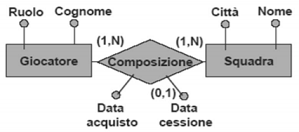
\includegraphics[scale=.75]{img/120.PNG}\end{center}

\subsubsection{Contenuto del gate e \emph{Global Descriptor Table}}  	
\begin{itemize}
	\item All'interruzione abbiamo sempre associato un tipo: in alcuni casi è stabilito dall'APIC (interruzioni esterne), in altri dall'operando di una istruzione (istruzione INT), in altri ancora è implicito (eccezioni).
	\item Il tipo permette di identificare un'entrata dell'IDT. Ciascuna entrata contiene delle informazioni. Quelle che ci interessano maggiormente sono:
	\begin{itemize}
		\item l'indirizzo della routine da mandare in esecuzione (nulla di nuovo);
		\item un bit I/T che indica il tipo del gate (\textit{interrupt} o \textit{trap}, nulla di nuovo);
		\item un flag $P$, che specifica se la routine è stata implementata o no;
		\begin{itemize} 
			\item Logicamente non saranno implementate tutte le 256 routine possibili.
			\item Se $P=0$ il processore non può attraversare il \emph{gate} e genera una nuova eccezione di tipo \emph{gate non implementato}. I programmatori di sistema solitamente implementano questa eccezione: se ciò non avviene il processore subisce una doppia eccezione (\emph{abort}) e si spegne. 
		\end{itemize}
		\item il \emph{Descriptor Privilege Level}, che indica il livello di privilegio minimo  che il processore deve avere prima di attraversare un certo gate;
		\begin{itemize}
			\item Notare che \textbf{con un'interruzione esterna e un'eccezione il gate viene attraversato comunque}, la limitazione sta solo nell'uso dell'istruzione INT. La cosa è utile per prevenire l'esecuzione attraverso INT di routine normalmente associate a interruzioni esterne e/o eccezioni.
		\end{itemize} 
	\item Un selettore di codice relativo a un'entrata della \emph{Global Descriptor Table}, quella del segmento dove si trova la routine.
	\end{itemize}
\end{itemize} 

\paragraph{A cosa ci serve il selettore di codice?} Per trovare il livello di privilegio dopo aver attraversato il gate. Detto in altro modo: cosa dobbiamo scrivere nel \emph{Current Privilege Level} dopo aver attraversato il gate?
	\begin{itemize}
		\item  L'informazione non si trova nella tabella delle interruzioni ma nella \emph{Global Descriptor Table} (GDT), tabella legata al meccanismo della segmentazione. La tabella, dato il segmento codice dove si trova la routine, indica una serie di informazioni:
		\begin{itemize}
			\item da che indirizzo parte;
			\item quanto è grande il segmento;
			\item \textbf{il livello di privilegio}!
		\end{itemize} 
		\item Il meccansimo della Intel è flessibile: si da la possibilità di decidere se innalzare o no il livello di privilegio: ciò per noi è una semplice constatazione, innalzeremo sempre il livello di privilegio.
	\end{itemize} 
%\paragraph{Come raggiungiamo la relativa entrata nella GDT?} Nella IDT troviamo il relativo selettore di codice (\emph{code selector}) relativo al segmento di codice dove si trova la routine.
	\clearpage
\subsubsection{Necessità di una nuova pila}
Alcune informazioni vengono memorizzate in pila. Non possiamo utilizzare in modalità sistema il contenuto di una pila manipolato dall'utente (non possiamo fidarci dell'utente, MAI). Segue la necessità di fare un cambio di pila qualora vi sia un cambio di privilegio.\begin{itemize}
	\item Distinguiamo due pile: la \emph{pila utente} e la \emph{pila sistema}.
	\item \textbf{Se il livello di privilegio si innalza il processore passa da pila utente a pila sistema} (si confronta il \emph{Current Privilege Level} col nuovo livello di privilegio trovato nella \emph{Global Descriptor Table}). Cambiare pila significa modificare il valore del registro RSP. Nella pila sistema andiamo a porre delle informazioni: 
	\begin{center}
		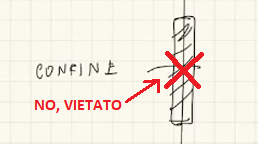
\includegraphics[scale=.8]{img/283.PNG}
	\end{center}
	\begin{enumerate}
		\item il vecchio RIP.
		\item il vecchio registro CS (in particolare il vecchio CPL);
		\item i vecchi flag (RFLAGS);
		\item il vecchio RSP (cioè dov'era RSP prima di fare il passaggio);
		\item il selettore pila vecchio (che non ci interessa poichè legato alla segmentazione);
	\end{enumerate}
	queste informazioni rendono possibile il ritorno nella pila utente.
	\item Salvate tutte queste informazioni il processore preleva dal gate il nuovo RIP e il nuovo CS (in particolare il nuovo CPL). 
	\item La IRETQ confronta il \emph{Current Privilege Level} e il CPL preso dal vecchio valore di CS in pila. Per prima cosa si verifica che il vecchio valore sia al più uguale (e non maggiore) del CPL attuale (controllo necessario per impedire violazioni del meccanismo della protezione\footnote{L'utente potrebbe fare casini modificando RSP prima di lanciare la IRETQ.}). Successivamente si verifica se è necessario riportare in RSP la pila utente (confronto tre \emph{Current Privilege Level} e il CPL preso dal vecchio valore di CS in pila). La IRETQ ripristina ciò che va ripristinato recuperando le informazioni dalla pila corrente (quella puntata con RSP). 
\end{itemize}
\paragraph{Osservazione} \emph{pushf} e \emph{popf} non permettono l'alterazione di tutti i flag. Abbiamo visto che per modificare il trap flag utilizziamo una funzione con istruzioni \emph{pushf} e \emph{popf}. Quindi è possibile modificare qualunque flag in questo modo? No, \emph{iretq} e \emph{popf} non permettono la sovrascrizione di tutti i flag: contrariamente ad altre situazioni non si ha un'eccezione, semplicemente si ignorano le richieste di modifica senza effetti visivi.

\subsubsection{Da dove viene preso il puntatore alla nuova pila?} 
L'Intel nel 286 prevedeva la possibilità di gestire la microprogrammazione quasi completamente in hardware (anche questa cosa sostanzialmente non usata). Dai GDT è possibile raggiungere i \emph{Task State Segment} (TSS). Questi segmenti, previsti di suo dal processore Intel e identificati da una certa entrata della GDT, contengono informazioni relative a un particolare programma in esecuzione. Inoltre si ha un registro \emph{Task Register} (TR) contenente l'indice del \emph{task/job} corrente. Nel TSS si hanno tante informazioni, tra queste \textbf{il puntatore \underline{alla base} della pila sistema}. 
\begin{center}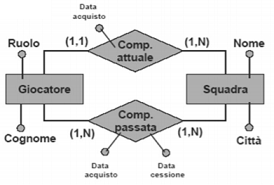
\includegraphics[scale=.75]{img/121.PNG}\end{center}
Quando c'è un'interruzione il processore usa TR per accedere al segmento TSS a partire dalla GDT, trovando così l'indirizzo della pila sistema.

	
\subsection{Livello di privilegio e istruzioni IN/OUT/CLD/STD (flag IOPL)}
Le istruzioni IN/OUT/CLD/STD non sono automaticamente vietate a livello utente. Esiste un altro campo, nel registro dei flag, detto \emph{IO Privilege Level} (IOPL), che per noi assume come valore 
\begin{multicols}{2}
\begin{itemize}
	\item $00$ (sistema) o
	\item $11$ (utente).
\end{itemize} 
\end{multicols} \noindent Con questo definiamo il livello privilegio che dobbiamo avere per eseguire le istruzioni IN/OUT/CLD/STD. L'informazione è statica e rimane lì anche dopo passaggi di gate. Le modifiche al campo sono ignorate nell'esecuzione di POPF e IRETQ. 

\subsection{Morale della favola}
\begin{framed}
\noindent Per far funzionare le interruzioni abbiamo bisogno di:
	\begin{itemize}
		\item almeno un segmento TSS (ci serve un solo TSS per gestire i passaggi tra due livelli di privilegio),
		\item almeno un descrittore nella GDT,
		\item e il registro TR inizializzato in modo da contenere l'identificativo di questo descrittore. 
	\end{itemize}  Fortunatamente possiamo fare questa cosa all'avvio.
\end{framed}
\clearpage

\section{Esempio di programma: passaggio a livello utente (\emph{liv$\_$utente})}
\paragraph{Perchè ci interessa questa cosa?} Il nostro programma parte in modalità sistema, a un certo punto vogliamo passare in modalità utente. La IRETQ da sola non basta, dobbiamo impostare la pila nei modi detti prima per compiere il cambio di privilegio.
\paragraph{Esempio} Supponiamo di voler eseguire la seguente funzione due volte: la prima volta in modalità sistema e la seconda in modalità utente.
\begin{verbatim}
	void foo() {
		    natb c;
		    printf("Provo a leggere RBR\n");
		    c = inputb(0x60);
		    printf("Ho letto RBR: %2x\n", c);
	}
\end{verbatim}
Gestiamo il passaggio a livello utente attraverso la funzione \emph{liv$\_$utente}, che poniamo nel nostro codice tra le due chiamate di \emph{foo}.
\begin{verbatim}
	foo();
	liv_utente();
	foo();
\end{verbatim}
\begin{center}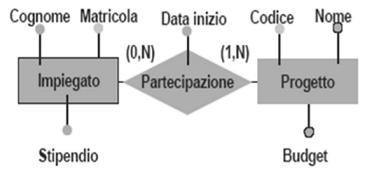
\includegraphics{img/122.PNG}\end{center}
La funzione si bassa sulla necessità di passare dalla IRETQ per effettuare un passaggio da modalità sistema a modalità utente. Sappiamo che la IRETQ recupera del contenuto dalla pila e lo utilizza: segue che per utilizzare la IRETQ dovremo mettere in pila ciò che la funzione si aspetta. Le cose sono quelle già elencate prima
\begin{enumerate}
	\item Tolgo l'indirizzo di ritorno con la pop
	\item Pongo il selettore dati utente (il vecchio contenuto del registro SS, non ci interessa)
	\item Pongo l'RSP
	\item Pongo il registro dei flag aggiornato
	\item Pongo il selettore codice utente (il contenuto del registro CS, ci interessa il CPL)
	\item Pongo l'indirizzo di ritorno rimosso all'inizio
	\item Chiamo la IRETQ
\end{enumerate}
\begin{center}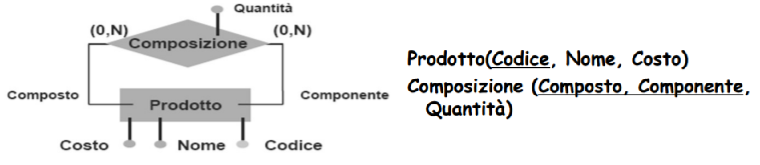
\includegraphics{img/123.PNG}\end{center}
A questo punto ogni istruzione che richiede un livello di privilegio maggiore rispetto a quello corrente provocherà il lancio di un'eccezione di tipo 13 (\emph{eccezione di protezione}). L'eccezione è di tipo \emph{fault}, dunque l'indirizzo stampato del warming è quello dell'istruzione che ha causato il problema (la IN). 

\part{Nucleo multiprogrammato didattico}

\chapter{Introduzione}
Con nucleo multiprogrammato intendiamo un sistema in grado di svolgere più \emph{processi}.
\begin{center}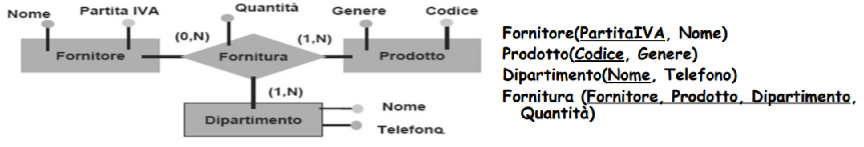
\includegraphics[scale=.80]{img/124.PNG}\end{center}
Il sistema che creiamo fornisce ai suoi utenti due astrazioni: \emph{processi} e \emph{primitiva}. Il meccanismo che realizza queste due astrazioni è detto \emph{contesto}.
\section{Concetti base}
\subsection{Processo} Il processo è \underline{un programma in esecuzione}. 
\[\text{Processo} \neq \text{Programma}\]
Pensiamo al pizzaiolo inesperto che sta facendo la pizza: ha bisogno di una ricetta, perché non si ricorda come si fa.
\begin{itemize}
\item La ricetta è il programma, che posso utilizzare per creare le pizze (anche in contemporanea).
\item Il pizzaiolo è il processore, la pizza i dati (l'input è la richiesta del cliente).
\end{itemize}
\textbf{Nessuna di queste cose è il processo}. Il processo possiamo immaginarlo come il filmato di tutto ciò che accade in questo sistema (\emph{pizza + pizzaiolo}), dall'inizio alla fine (il filmato di tutti gli stati attraverso cui il sistema passa).
\paragraph{Usciamo dalla metafora} Il processo è la sequenza degli stati attraverso cui passa il sistema eseguendo il programma. L'esecuzione di ogni istruzione del programma fa passare il processo da uno stato al successivo.
\paragraph{Programma vs Processo} Può essere facile confondere il processo col programma.
\begin{itemize}
	\item Un programma può essere eseguito da più processi "contemporaneamente". I clienti chiedono la pizza margherita, il pizzaiolo ne fa tante, ognuna di queste segue il suo processo indipendentemente dalle altre. 
	\item Un processo può eseguire programmi diversi. Si pensi alla \emph{pizza al metro}, con vari tipi di pizza uno dietro l'altro.
\end{itemize}
\paragraph{Fotogramma} 
\begin{itemize}
\item Concentriamoci sul fotogramma: pur avendo una sequenza di stati possiamo concentrarci su uno stato in un particolare istante. \textbf{Per la natura dei nostri processi dato un qualunque fotogramma avrò le informazioni necessarie per proseguire il processo} (di ogni pizza il pizzaiolo si ricorda dove è arrivato).
\item Passare da un processo a un altro significa ricordarsi il fotogramma dove è arrivato il processo da cui stiamo saltando via, caricarlo e spostarci sul fotogramma del nuovo processo che vogliamo portare avanti.
\end{itemize} Il processo è una cosa sequenziale. \textbf{Non possiamo, tuttavia, definire il processo come l'istanza di un programma}: un processo, ricordiamolo, può cambiare programma. 
\begin{itemize}
	\item  Il programma non è la sceneggiatura del processo: la ricetta può contenere delle varianti (quattro stagioni con o senza carciofi...). Il processo di produzione di una singola pizza riguarda una sola delle varianti possibili.
	\item Il programma potrebbe contenere dei cicli. Nel programma vediamo le azioni ripetute una volta sola, mentre nel processo vediamo le azioni effettivamente ripetute tante volte.
\end{itemize}

\subsection{Primitiva}
\paragraph{Cosa intendiamo con \emph{primitivo}} Primitivo è un qualcosa di \textit{non derivato}, un mattone fornito dal sistema per costruire il resto delle cose. L'esempio sono le funzionalità di base fornite da un programma di grafica. Ricordarsi la caratteristica fondamentale delle primitive:
\[\boxed{\text{La primitiva non è scomponibile.}}\]
\paragraph{Funzioni di libreria?} Si potrebbe dire che le primitive sono funzioni di libreria non scomponibili (di solito lo sono).
\paragraph{Tipi primitivi} I tipi primitivi di un linguaggio (int, long, char...) sono offerti dal linguaggio, possono essere usati per definire nuovi tipi derivati, ma non possono essere modificati nel comportamento.

\paragraph{Cosa faremo a breve} Creeremo un sistema che fornisce una stazione dei processi, esegue programmi all'interno dei processi, fornisce delle primitive che sono le funzionalità di base presenti all'interno di questi programmi.
\begin{itemize}
	\item Gli utenti possono lanciare le primitive e usufruire dei servizi da esse offerte.
	\item Normalmente le primitive di un sistema sono pensate come {chiamate di sistema}, dunque con privilegio maggiore. Le primitive molto spesso reggono il loro funzionamento su delle strutture dati: queste strutture dati non devono essere manipolabili dall'utente, o al più manipolabili in modo controllato (non raggiungibili dal livello utente se non attraverso una primitiva).
	\item Gli utenti non possono manipolare le primitive esistenti, ma soprattutto non possono crearne di nuove.
\end{itemize}

\subsection{Contesto}
Con la parola contesto si intende, nel linguaggio comune, tutto ciò che è necessario sapere per interpretare correttamente un dato testo, ma che non è scritto esplicitamente nel testo stesso. Prendiamo ad esempio la seguente istruzione C++:
\begin{verbatim}
	x = x + 1
\end{verbatim}
abbiamo una somma, ma non sappiamo in cosa consista \emph{x}.

\paragraph{E nel nostro caso?} Il contesto permette la realizzazione delle astrazioni \emph{processo} e \emph{primitiva}. Se io ho più processi che vanno avanti, anche processi che eseguono lo stesso programma, avrò per ciascuno uno stato. (i registri relativi a un processo potrebbero non essere i registri relativi a un altro processo). \textbf{In un certo senso il \emph{contesto} consiste nello stato del processo}. Associo un contesto diverso ad ogni processo (nel nucleo faremo ciò con un \emph{descrittore di processo}).
\paragraph{Cambio di contesto}
Quando si passa da un processo a un altro si dice che \emph{si cambia contesto}. Il processore, chiaramente, può dedicarsi a un solo processo alla volta: l'unico modo per avere un'esecuzione apparentemente concorrente dei processi è eseguire in modo frammentato i processi (eseguo un pezzo di un processo, cambio contesto, eseguo un pezzo di un altro processo, cambio nuovamente contesto, e così via...)
\paragraph{Contesto e primitive}
Questa idea di contesto è valida anche per le primitive: supponiamo di avere un'istruzione HLT, è lecito o non è lecito eseguirla? Di per sè non è nè lecita, nè illecita. Dipende solo da chi la vuole eseguire: un utente non ne ha diritto, il sistema sì. Anche l'invocazione di primitiva da parte di un processo può essere immaginato come un \emph{cambio di contesto} (meno drammatico rispetto al cambio di contesto vero e proprio), che definiamo \emph{cambio di privilegio} per distinguerlo dai cambi di processo.

\section{Moduli} Il sistema che andiamo a studiare è realizzato in moduli: ogni modulo è un programma a se stante eseguito in un contesto (di privilegio) diverso. 
\begin{itemize}
\item Il \textbf{modulo sistema} deve essere eseguito a livello sistema;
\item Il \textbf{modulo I/O} è eseguito a livello sistema (la soluzione ideale sarebbe eseguirlo a un livello di privilegio intermedio, ma abbiamo solo due modalità - sistema e utente);
\item Il \textbf{modulo utente} è eseguito a livello utente. 
\end{itemize}
In sostanza...
\begin{itemize}
	\item Il programmatore di sistema scrive delle primitive, che svolgono operazioni per conto dell'utente (impedisco all'utente di occuparsi delle periferiche, ad esempio, ma gli dico che posso farlo io). Il codice di sistema, così come le primitive e le strutture dati su cui si reggono, sono posti nel modulo sistema e nel modulo I/O (vedremo verso la fine l'utilità del modulo I/O). 
	\item Le primitive possono essere invocate esclusivamente passando da un gate della IDT, innalzando il livello del processore.  
	\item L'utente si scrive i programmi di cui ha bisogno e li esegue in modalità utente, facendo eventuale ricorso alle primitive offerte dal nucleo. 
\end{itemize} Il modulo sistema e il modulo I/O costituiscono, di fatto, un sistema operativo non modificato dall'utente, che riceve il programma e lo esegue.

\section{Cartelle}
\paragraph{Modulo sistema} I file che compongono il modulo sistema stanno nella directory 
\begin{verbatim}sistema\end{verbatim}
tutto è posto in due file: \emph{sistema.cpp} (parte C++) e \emph{sistema.s} (parte Assembler). 

\paragraph{Modulo I/O} I file che compongono il modulo I/O stanno nella directory
\begin{verbatim}io\end{verbatim}
anche in questo caso abbiamo tutto in due file: \emph{io.cpp} (parte C++) ed \emph{io.s} (parte Assembler).

\paragraph{Modulo utente} I file che compongono il modulo utente stanno nella directory
\begin{verbatim}utente\end{verbatim}
abbiamo più files: 
\begin{itemize}
\item \emph{all.h}
\item \emph{lib.cpp}
\item \emph{lib.h}
\item \emph{utente.s}
\item \emph{utente.cpp}
\end{itemize}
La cosa è necessaria per permettere all'utente di scrivere solo la parte che gli interessa (quella C++, nell'ultimo file). 

\paragraph{Approccio} L'approccio è il solito: utilizzare Linux come sistema di appoggio per \emph{cross-compiling}.  Compiliamo su Linux programmi pensati per girare come sistema. 

\section{Esempio di scrittura del file \emph{utente.cpp}:  Hello, world!}
\small
\begin{verbatim}
#include <all.h>

void main() {
    writeconsole("Hello, world!\n", 14);
    pause(); /* Per evitare che il processo venga terminato subito */
    terminate_p();
}
\end{verbatim}
\normalsize
\begin{itemize}
\item Includiamo \emph{all.h} per avere a disposizione tutte le funzioni.
\begin{verbatim}
#include <costanti.h>
#include <libce.h>
#include <sys.h>
#include <io.h>
#include "lib.h"
\end{verbatim}
\item Scriviamo il \emph{main}, che non è standard (attenzione al \emph{void}). Il sistema lo esegue all'interno di un processo: quando il processo termine e non ci sono altre cose da fare il sistema spegne la macchina.
\item Un esempio di primitiva è \emph{writeconsole}
\begin{verbatim}
writeconsole("Hello, world!\n", 14);
\end{verbatim}
passiamo la stringa e indichiamo la sua lunghezza.
\item \emph{terminate$\_$p} è un altro esempio di primitiva, invocata per terminare esplicitamente il processo.
\item Si osservi che entrambe le primitive comportano un cambio di privilegio: la prima sarà eseguita dal modulo I/O (poichè posta nel modulo I/O), la seconda dal modulo sistema (poichè posta nel modulo sistema).
\end{itemize}
%\section{tbd}
%Il processore Intel si fa tutta la storia dei processori Intel dall'8086 all'AMD64, cioè parte in una modalità sostanzialmente compatibile con l'8086 (a 16 bit, senza protezione), attraverso dei registri di controllo passa a una modalità compatibile col 386 (a 32 bit), e infine si pone in una modalità compatibile con l'AMD64 (a 64 bit). I programmi da noi scritti (e il modulo sistema) partono suppendo che il processore sia già nell'ultima modalità dunque il bootloader deve portarci in questa modalità (il primo passaggio a 32 bit se ne occupa QEMU, quello da 32 bit a 64 bit lo fa il bootloader). A questo punto vengono posti in memoria i segmenti del file ELF \emph{sistema}, e cede il controllo. Il file ELF \emph{sistema}, dopo essere stato caricato, interpreta gli altri due file rimanenti (\emph{IO} e \emph{utente}): questa cosa deve farla per forza lui.
\section{Compilazione e avvio del sistema}
Eseguiamo il comando \emph{make} nella root
\begin{verbatim}
make
\end{verbatim}
la procedura ha creato, nella cartella \emph{build} tre file ELF: modulo utente, modulo sistema e modulo I/O. Ribadiamo che ciò che abbiamo ottenuto non è pensato per essere eseguito su Linux ma su un'altra macchina avente architettura comune.
 

\paragraph{Avvio del sistema}
\begin{itemize}
\item Il modulo sistema è il primo modulo caricato dal bootloader. Il modulo sistema questa volta è un po' più sofisticato: inizializza le sue strutture dati, prepara i moduli I/O e utente. Il bootloader si limita solo a caricare questi moduli in memoria, il modulo sistema li interpreta. Quando è tutto pronto viene creato un nuovo processo e si avvia l'esecuzione del programma \emph{main} in quel processo, a livello utente. 
\item Osserviamo che all'avvio viene inizializzata la GDT (accompagnata da alcuni elementi della segmentazione necessari per definire i livelli di privilegio), l'APIC, il timer (che restituisce periodicamente il controllo al sistema). il modulo IO con tutte le periferiche che conosciamo (tastiera, video, busmaster). Dopo tutte queste inizializzazioni passo il controllo all'utente.
\item Ogni processo è identificato da un numero, visibile nel terminale (dei vari messaggi e warning si vede il relativo processo) .
\item Il processore esegue il sistema o il modulo utente. Risponde a tutte le chiamate di sistema che l'utente potrebbe fare, e a tutte le eccezioni/interruzioni, che provocano la restituzione del controllo al modulo sistema (o al modulo I/O in alcuni casi).
\end{itemize}

\section{Esempio di programma bloccato dalla protezione}
\small
\begin{verbatim}
#include <all.h>

void main() {
    volatile natw* video = (natw*)0xb8000;
    video[4] = 0x3F00 | `a';
    
    pause(); /* Per evitare che il processo venga terminato subito */
    terminate_p();
}
\end{verbatim}
\normalsize
\begin{itemize}
\item Proviamo a scrivere in memoria video senza utilizzare la primitiva \emph{writeconsole}.
\item Se compiliamo non succede nulla, ma quando avvieremo il sistema il nostro programma verrà interrotto. Nel momento in cui ha provato a scrivere in quella zona di memoria il processore si è rifiutato e ha lanciato un'eccezione 14 di \emph{page fault}: il controllo è stato restituito al sistema, la routine andata in esecuzione ha interrotto il processo e stampato una miriade di informazioni (che dovrebbero aiutarci a capire in che stato si trovava il processo al momento dell'errore).
\begin{center}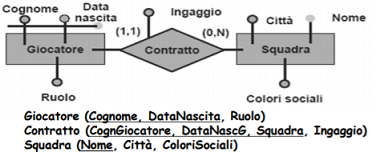
\includegraphics[scale=.85]{img/125.PNG}\end{center}
Vediamo che l'eccezione è stata provocata da una certa riga di \emph{utente.cpp}, vediamo anche l'indirizzo di memoria relativo. Si indica il livello di privilegi corrente al momento di esecuzione dell'istruzione, i valori dei registri (RFLAGS, IF, IOPL, RAX, RBX...). Per quanto riguarda il registro RIP il log è automaticamente decodificato, se l'indirizzo è associabile a una riga del sorgente si pone direttamente il numero di riga. Possiamo evitare questa cosa nel seguente modo
\begin{verbatim}
CERAW=1 ./run
\end{verbatim}
\end{itemize}

\subsection{\emph{backtrace}} Il backtrace mostra lo stack delle chiamate. Proviamo a porre il programmino precedente nel seguente modo:
\small
\begin{verbatim}
#include <all.h>
void f1() {
    volatile natw* video = (natw*)0xb8000;
    video[4] = 0x3F00 | `a';
}

void f2() { f1(); }

void main() {
    f2();
    pause(); /* Per evitare che il processo venga terminato subito */
    terminate_p();
}
\end{verbatim}
\normalsize
Otteniamo un lancio di eccezione anche in questo caso
\begin{center}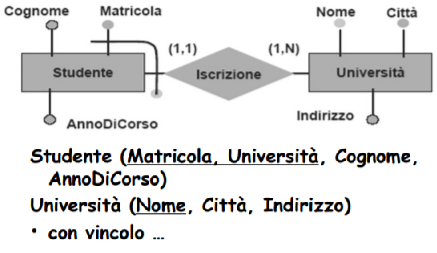
\includegraphics[scale=.85]{img/126.PNG}\end{center}
\begin{itemize}
\item Si specifica che al momento dell'errore l'instruction pointer era dentro \emph{f1}.
\item Si indica che \emph{f2} è stata chiamata da \emph{f1},  a sua volta chiamata da \emph{main}. In entrambi i casi si indica la riga del sorgente con la chiamata. 
\end{itemize}
Il backtrace è utile perché la funzione potrebbe essere chiamabile da più punti del nostro sorgente.

\section{Libreria \emph{libce}}
\small
\begin{verbatim}
#include <all.h>

void f1() {
    char_write(`a');
}

void f2() { 
    f1(); 
}

void main() {
    f2();
    pause(); /* Per evitare che il processo venga terminato subito */
    terminate_p();
}
\end{verbatim}
\normalsize
Il nostro programma è collegato anche con la libreria \emph{libce}, stessa cosa il modulo I/O. Per scrivere su video i codici da scrivere sono i soliti già visti. Dobbiamo ricordarci che non è il codice a dirci il livello di privilegio, ma il contesto.

\chapter{Processo}

\section{Gestione dei processi}
\small
\begin{verbatim}
	#include <all.h>
	
	void f1() {
		    char_write(`a');
	}
	
	void f2() {
		    f1();
	}
	
	void main() {
		    natw id = activate_p(f1, 10, 40, LIV_UTENTE);
		    terminate_p();
	}
\end{verbatim}
\normalsize
Una delle cose che possiamo fare con questo sistema è gestire i processi.  Il sistema mi fornisce la primitiva \emph{activate$\_$p}, che mi permette di attivare un nuovo processo. Devo indicare
\begin{itemize}
	\item la funzione che dovrà eseguire questo processo,
	\item gli eventuali parametri in ingresso,
	\item la precedenza (si esprime come valore numerico),
	\item il livello di privilegio (in realtà la primitiva non ci concederebbe la creazione di un processo sistema, solo che questa cosa può essere utilizzata dal modulo I/O, che può chiedere di creare un processo a livello sistema).
\end{itemize}
La decisione di quali processi vanno avanti e quando è una delle questioni più bollenti riguardo i sistemi operativi. 
\paragraph{Identificativo del processo} La funzione restituisce un valore: l'identificatore del processo appena creato. Restituisce una sequenza di $1$ nel caso in cui ci siano stati errori.

\paragraph{Che differenza c'è tra \emph{printf} e \emph{writeconsole}?} La \emph{printf} è una libreria di funzione che per stampare caratteri userà delle primitive. La \emph{writeconsole} è una primitiva vera e propria.

\paragraph{Come si realizza l'astrazione dei processi?}
Durante la sua vita un processo può trovarsi in uno tra diversi stati di esecuzione. Il processore sta eseguendo le istruzioni del programma, sta portando avanti lo stato del processo.  Se abbiamo un solo processore solo un processo può trovarsi nello stato \textbf{esecuzione}. Tutti gli altri processi presenti nel sistema possono trovarsi in uno tra i seguenti stati:
\begin{itemize}
	\item \textbf{pronti} (il processo potrebbe andare avanti se dipendesse solo da lui, non va avanti perché il processore è già occupato da qualcun'altro con precedenza maggiore),
	\item \textbf{bloccati} (il processo sta attendendo il verificarsi di un certo evento, per esempio il termine di un'operazione di I/O, non può andare avanti neanche col processore libero).
\end{itemize}
Supponiamo di avere due processi: \emph{job1} e \emph{job2}, il primo ha precedenza maggiore.
\begin{center}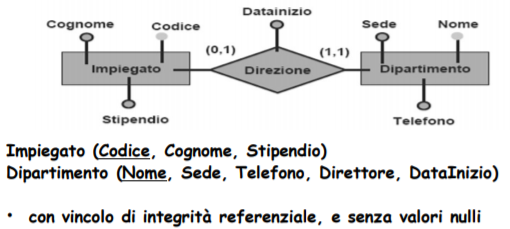
\includegraphics[scale=.75]{img/127.PNG}\end{center}
\begin{itemize}
	\item Si inizia con l'esecuzione di \emph{job1}, che ha priorità maggiore. Rimane in stato \emph{esecuzione} finchè non avvia l'operazione di I/O output. A quel punto il \emph{job1} si pone nello stato \emph{bloccato} e passa la palla a \emph{job2}.
	\item Il processo \emph{job2} passa in \emph{esecuzione}. Si eseguono istruzioni finchè l'operazione di I/O non risulta completata. A quel punto si ha una richiesta di interruzione intercettata dal sistema: la routine rimette \emph{job1} in \emph{esecuzione} e pone \emph{job2} nello stato \emph{pronto}.
	\item Il processore conclude l'esecuzione di \emph{job1} invocando una primitiva di sistema: a quel punto si rimette in \emph{esecuzione} il processo \emph{job2}.
\end{itemize}
I passaggi sono intramezzati per forza di cose, abbiamo numerose variazioni di stato dei vari processi. Si parla di:
\begin{center}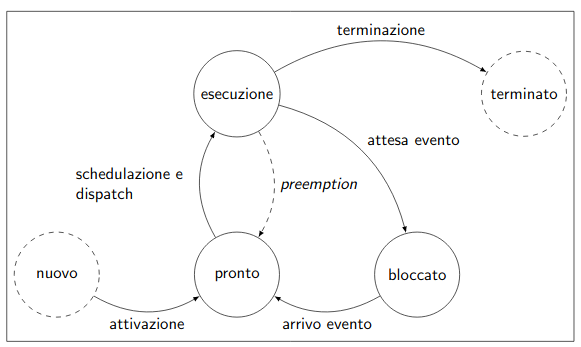
\includegraphics[scale=.76]{img/198.PNG}\end{center}
\begin{itemize}
	\item \textbf{schedulazione}, quando un processo passa da \emph{pronto} a \emph{esecuzione};
	\item \textbf{blocco}, quando un processo passa da \emph{esecuzione} a \emph{bloccato};
	\item \textbf{risveglio}, quando un processo passa da \emph{bloccato} a \emph{esecuzione};
	\item \textbf{preemption}, quando un processo passa da \emph{esecuzione} a \emph{pronto},.
\end{itemize}
L'ultimo passaggio, che possiamo italianizzare in \emph{prelazione}, avviene quando è possibile eseguire processi con priorità maggiore. La cosa non è presente in tutti i sistemi multiprocesso.
\paragraph{Conseguenza di questa assenza}  Un processo va avanti finchè non si blocca, ma per bloccarsi è lui che chiama una primitiva di sistema. Se fa un ciclo infinito il processore rimane lì. Se c'è un errore in un programma  tutto il sistema si blocca (ripensare a sistemi operativi come \emph{Windows 95 / 98 / ME}). In un sistema del genere il processore si accorge di processi con priorità maggiore solo dopo che il processo in esecuzione è stato bloccato.
\paragraph{Creazione di processi} Un processo può creare altri processi assegnando una priorità minore o maggiore. Se il processo ha priorità maggiore potrebbe fare \emph{preemption} subito. Nel nostro caso non sarà così perché imporremo la creazione di processi aventi priorità minore.
\paragraph{Terminazione dei processi} Il processo può essere terminato solo mediante esecuzione di primitiva, dunque il processo dovrà essere in \emph{esecuzione}. Per permettere a processi di uccidere altri processi dobbiamo implementare ulteriori meccanismi che non ci interessano. Distinguiamo la cosa da una terminazione dovuta a eccezioni.

\paragraph{Sistema come intermediario} I cambi di processo avvengono grazie all'intermediazione del sistema: avvengono solo quando i processi, che normalmente girano a livello utente, sono passati a livello sistema (con uno dei metodi possibili, per eccezione, interruzione esterna o istruzione INT). Tutto ciò è vero per tutti i sistemi multiprogrammati. 

\paragraph{Semplificazioni} Il nostro sistema adotta alcune semplificazioni:
\begin{itemize}
\item una schedulazione che si basa solo sulle precedenze dei processi;
\item il sistema è multiprocesso ma non multiutente.
\end{itemize}
La multiprogrammazione si è resa necessaria andando avanti: è vero che l'utente è unico, ma è vero che l'utente singolo vuole fare più cose in simultanea. L'utente, inoltre, esegue programmi non realizzati da lui, ed esegue in simultanea programmi realizzati da sviluppatori diversi.
\clearpage 

\section{Processo dal punto di vista dell'utente}
Un'altra cosa su cui i sistemi possono distinguersi è quanta memoria i processi possono condividere tra di loro (condividere nel senso avere processi con dati in comune). Abbiamo sistemi \emph{a scambio di messaggi} (dove non si condivide niente) e sistemi \emph{a memoria comune} (dove condividono tutto). Quello che faremo noi è un ibrido.
\begin{itemize}
\item \textbf{Parte condivisa}. 

I processi condividono tutto ciò che è globale nel modulo utente
\begin{verbatim}
.text
.data
.bss
.heap // anche lo heap, creato a tempo di esecuzione
\end{verbatim}
\item \textbf{Parte non condivisa}.

Ogni processo presenta una \emph{pila privata}.
\end{itemize}
Le pile sono separate in modo netto: un processo non ha la possibilità di accedere alla pila di un altro processo.

\section{Processo dal punto di vista del programmatore}
Dal punto del sistema abbiamo un programmatore, non un utente, che prepara le strutture dati e le routine necessarie per realizzare quanto visto dall'utente. Ogni processo è descritto da una \emph{struct}: il \textbf{descrittore di processo}
\begin{verbatim}
des_proc *pronti;
des_proc *esecuzione; // <--- uno solo, visto che abbiamo solo un processore
const int N_REG = 16;

struct des_proc {
    natw id;
    natw livello;
    natl precedenza;
    vaddr punt_nucleo; /* Puntatore a pila sistema */
    natq contesto[N_REG];
    paddr cr3;
    
    des_proc *puntatore;
};
\end{verbatim}
\begin{itemize}
	\item \textbf{esecuzione}. Una variabile globale (il puntatore \emph{esecuzione}) si ricorda del processo in esecuzione (ricordiamo, uno solo se abbiamo un solo processore).
	\item \textbf{punt$\_$nucleo}. Il sistema oltre ad avere un descrittore di processo per ogni processo ha anche una pila sistema diversa per ogni processo. perché? Abbiamo detto che ogni processo deve avere la sua pila: la cosa è valida non solo in modalità utente, ma anche in modalità sistema. Tutte le informazioni che il processore salva quando attraversa un gate devono rimanere sulla pila del processo, poichè costituiscono lo stato del processo quando si verifica l'interruzione/eccezione/int (tutte cose che dobbiamo tenere da parte).
\item \textbf{contesto}. La cosa più importante che il sistema deve ricordarsi, di ogni processo, è "l'ultima foto" del suo sistema, che consiste in particolare nel contenuto dei registri. Abbiamo un array \emph{contesto} nella struttura, che contiene il valore corrente di tutti i registri del processore (ci semplifichiamo la vita non memorizzando lo stato della memoria).
\item \textbf{puntatore}. All'interno della struttura abbiamo \emph{puntatore}, un puntatore necessario per costruire delle liste che rappresentano tutti i processi che si trovano nei vari stati. 
\begin{itemize}
\item \textbf{pronti}. Tutti i processi pronti si trovano in una lista: il nostro sistema avrà una variabile globale (il puntatore \emph{pronti}) che punta al primo elemento della lista. I vari elementi che costituiscono la lista sono le strutture \emph{des$\_$proc}. La lista è ordinata in base al campo \emph{precedenza} del processo, segue che per l'operazione di \emph{schedulazione} basterà leggere il primo elemento della lista (cosa con complessità nulla).
\item Esistono più liste dedicate ai processi bloccati, ciascuna riguardante uno specifico evento: lista per chi aspetta di utilizzare l'hard disk, chi la tastiera, chi il timer...
\end{itemize}
Queste liste sono gestite dal sistema, dopo aver ottenuto nuovamente il controllo a seguito del passaggio del gate (ricordiamoci, serve l'atomicità per manipolare delle liste).
\item \textbf{cr3}. Affrontato più avanti, nel capitolo sulla paginazione.
\end{itemize}
\paragraph{Differenze tra routine di sistema e routine di interruzione} 
\begin{itemize}
\item Possiamo immaginarci una routine di sistema come una routine di interruzione.
\item La differenza sostanziale sta nella proprietà di \emph{atomicità} della routine di sistema, ossia la sua indivisibilità. \textbf{La routine di interruzione può essere interrotta da un'altra interruzione, la routine di sistema no}!
\item \textbf{La routine di sistema non può essere considerata parte del processo} poichè non contribuisce all'avanzare dello stato del processo stesso.
\end{itemize}
\subsection{Passaggio a contesto sistema} Quando il processo passa il gate viene fotografato lo stato del processo corrente.  Il passaggio al \emph{contesto sistema} avviene con il seguente codice Assembler
\begin{verbatim}
CALL salva_stato
// ...
// codice della routine di sistema
// ...
CALL carica_stato
IRETQ
\end{verbatim}
\begin{itemize}
\item Con la \emph{salva$\_$stato} è una routine scritta in assembler che salva, nel campo \emph{contesto} del processo in esecuzione, lo stato dei registri.
\item Questo codice in realtà è il solito incapsulamento che abbiamo già usato altre volte. Non ci piace programmare in Assembler, dunque tra le due call chiameremo una routine implementata in C++. Ricordarsi che l'incapsulamento via Assembler è obbligatorio a causa della IRETQ (come la chiamiamo in C++? Non si può).
\item Con la \emph{carica$\_$stato} poniamo il contenuto del campo \emph{contesto} (del processo in esecuzione) nei vari registri.
\end{itemize}
\paragraph{Ribadiamo}
\[\boxed{\text{Quanto posto tra le due call non deve essere considerato parte del processo.}}\]
\subsection{Passaggio da un processo a un altro attraverso routine di sistema} Il passaggio da un processo a un altro è cosa semplice a questo punto. Abbiamo un codice simile al precedente (il passaggio avviene mediante routine di sistema, visto che il tutto funzione con l'intermediazione del sistema)
\begin{verbatim}
CALL salva_stato
// ...
esecuzione = ...
// ...
CALL carica_stato
IRETQ
\end{verbatim}
ma modifichiamo tra le due call il valore del puntatore \emph{esecuzione} (il valore precedente sarà posto in un'altra coda). Quando la nostra routine di sistema finisce la \emph{carica$\_$stato}  andrà a porre nei registri il \emph{contesto} del nuovo processo puntato dalla variabile globale \emph{esecuzione} (\textbf{solo a questo punto avviene il passaggio}).

\paragraph{Memoria protetta} Dal punto di vista della protezione tutte queste strutture dati (descrittori di processo, pile di sistema, variabili globali \emph{pronti} ed \emph{esecuzione}) devono stare nella parte di memoria non accessibile agli utenti. Distinguiamo due aree di memoria:
\begin{itemize}
	\item le strutture dati, i descrittori di processo, le pile sistema stanno nell'area di memoria non accessibile all'utente;
	\item modulo utente e pila del processo corrente stanno nell'area accessibile all'utente (supponiamo ci sia una pila alla volta in memoria).
\end{itemize}

\subsection{Atomicità: perché la routine di sistema deve essere indivisibile?} 
Dal punto di vista della correttezza limitarsi a proteggere una parte di memoria non è sufficiente. Dobbiamo garantire l'\emph{atomicità} per evitare problemi.
%\paragraph{Premessa} Ricordiamo quanto visto nella lezione del 15 aprile. Abbiamo un programma principale, un'interruzione, una variabile \emph{fine} letta dal programma principale e modificata dalla routine di interruzione.
%\begin{center}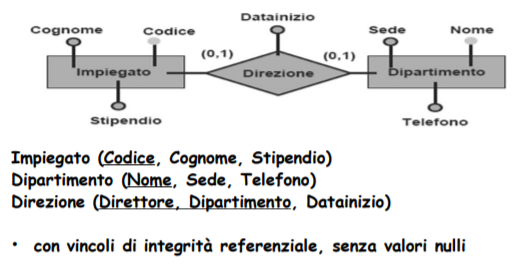
\includegraphics[scale=.55]{img/128.PNG}\end{center}
%La cosa si risolve ponendo la keyword \emph{volatile}. Quanto detto è il caso più semplice di condivisione di variabili tra due flussi di controllo non sequenziali (cioè due flussi mescolabili in maniera arbitraria). Gestire le interruzioni non è cosa semplice, e nel caso di routine di sistema può provocare problemi. 
\paragraph{Singole istruzioni} Un'istruzione è per definizione indivisibile: abbiamo detto che le interruzioni si manifestano tra un'istruzione e un'altra, non durante l'esecuzione di una singola istruzione.
\paragraph{Consistenza delle liste} Prendiamo ad esempio la gestione delle liste con i processi, che è in mano al sistema (l'intermediario, prendiamo ad esempio la coda \underline{globale} \emph{pronti}). 
\begin{center}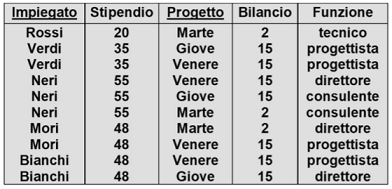
\includegraphics[scale=.65]{img/129.PNG}\end{center}
Abbiamo visto che la manipolazione della lista non richiede una semplice istruzione macchina, ma una serie di istruzioni durante le quali la lista non è consistente. La lista è consistente all'inizio (prima delle modifiche) e alla fine (dopo le modifiche). Lanciare un'interruzione nel bel mezzo della sua manipolazione significa considerarla in uno stato inconsistente (si hanno problemi se mentre stiamo manipolando una lista si ha un'interruzione e la relativa routine interviene anch'essa sulla lista che era in corso di modifica).  Ricordarsi che
\[\boxed{\text{La lista è consistente solo se tutti gli elementi sono raggiungibili partendo dalla testa}}\]
\paragraph{Cosa facciamo?} Seguono due strade possibili:
\begin{enumerate}
\item scrivere le routine pensando al fatto che lo stato considerato possa essere inconsistente (il programmatore normalmente scrive pensando che nessuno si metta di mezzo tra le istruzioni del suo programma);
\item impedire le interruzioni in modo tale che gli stati inconsistenti non siano visibili.
\end{enumerate}
La prima cosa è dispendiosa, la seconda semplice:
\begin{itemize}
	\item per le interruzioni esterne si ricorre a un apposito flag (il flag IF);
	\item le eccezioni devono essere evitate dal sistema;
	\item stessa cosa le interruzioni software (ad ogni chiamata di routine corrisponde una \emph{salva$\_$stato}, che sovrascrive il contesto precedente\footnote{Ricordiamo che ciò che viene eseguito in una routine di sistema non è parte di un processo. L'esecuzione di una \emph{salva$\_$stato} comporta la perdita delle informazioni relative alla routine eseguita.}).
\end{itemize}
 In questo modo evitiamo tutti i meccanismi che permettono di attraversare il gate e di ritornare ricorsivamente nel sistema. Possiamo dire che \textbf{la routine di sistema è diventata, in un certo senso, simile a un'unica istruzione di linguaggio macchina} (è atomica e indivisibile, viene eseguita fino alla sua fine). 

\paragraph{Wait, altro problema} Tenere disattivate le interruzioni \underline{è una limitazione troppo grande} per molti progettisti di sistema, dunque si è elaborata una via di mezzo. Nel modulo I/O, che vedremo più avanti, abbiamo un rilassamento delle restrizioni:
\begin{itemize}
	\item le eccezioni sono normalmente vietate;
	\item le interruzioni sono ammesse;
	\item la chiamate ricorsive sono permesse (forse si, forse no).
\end{itemize}
Tutto rimane vietato nel modulo sistema (atomicità, per forza).

\subsection{Prima istantanea dello stato di un processo} Per i processi appena partiti non è mai stata scattata una foto prima. La foto viene scattata quando si entra in modalità sistema: meccanismo delle eccezioni, processore (salva le informazioni nella pila sistema privata, per la IRETQ), in parte con la \emph{salva$\_$stato} (si aggiorna la struttura \emph{des$\_$proc}). Tutto questo funziona quando il processo esiste già e si attraversa un gate: ma per i processi appena creati? Il modo più semplice è fare in modo che l'\emph{activate$\_$p} generi la foto: 
\begin{verbatim}
	activate_p(miaproc, 10, 20, LIV_UTENTE);
\end{verbatim}
questo significa creare l'istanza relativa della struttura \emph{des$\_$proc} e allocare la pila di sistema.
\begin{itemize}
	\item Intanto posso impostare in \emph{des$\_$proc} la priorità e il livello di privilegio.
	\item Successivamente devo inizializzare il contesto e la pila in modo tale che le seguenti istruzioni, eseguite da una qualche routine, diano inizio al processo in modo regolare.
	\begin{verbatim}
		CALL carica_stato
		IRETQ
	\end{verbatim}
	\begin{itemize}
		\item In pila mettiamo 5 \emph{quadword} (la IRETQ vuole questo, ricordiamolo). Abbiamo:
		\begin{multicols}{2}
		\begin{itemize}
			\item (RIP) l'indirizzo della funzione da eseguire;
			\item (CPL) si imposta in modo che il livello di privilegio sia quello indicato nell'apposito parametro di ingresso;
			\item (RFLAG), si impostano i flag con IF ad 1 e IOPL sempre \textit{sistema} (si indica il \emph{Privilege level} necessario per eseguire certe istruzioni);
			\item (RSP), si pone l'indirizzo con la pila utente del processo in esecuzione;
			\item (TSS) cose relative ai segmenti che non ci interessano.
		\end{itemize}
		\columnbreak
		\begin{center}
			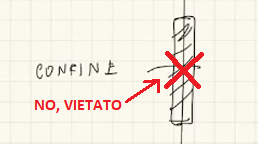
\includegraphics[scale=.8]{img/283.PNG}
		\end{center}
		\end{multicols}
		Si consideri che in un processo a livello sistema si crea solo la pila sistema, mentre in un processo a livello utente si crea sia la pila sistema che quella utente.
		\item Il contesto ha almeno due registri da inizializzare in modo preciso, gli altri possono essere uguali a zero.
		\begin{itemize}
			\item Il parametro in ingresso deve andare in RDI (la funzione \emph{miaproc} ha un parametro con valore $10$, lo mettiamo subito nel registro - secondo le regole già viste - per permettere l'esecuzione della funzione).
			\item Dobbiamo mettere in RSP l'indirizzo della pila sistema, in modo tale che IRETQ possa leggere i dati che abbiamo messo nella pila sistema.
		\end{itemize}
	\end{itemize}
	\item Si consideri che l'indirizzo della pila sistema non viene preso da \emph{des$\_$proc} ma da quella roba brutta vista qualche lezione fa: passaggio dal TR (\emph{Task Register}) per arrivare alla GDT (\emph{Global Descriptor Table}) e infine al TSS (\emph{Task State Segment}). Per indicare al processore di usare una certa pila abbiamo due strade...
	\begin{itemize}
		\item \textbf{Un TSS per processo}.
		
		Uso il meccanismo della segmentazione progettato da Intel (quindi \emph{punt$\_$nucleo} punta al TSS) come descrittore di processo (però a quel punto ci serve un TSS per ogni processo e siamo limitati nel numero a causa degli ingressi limitati della GDT) e cambiare ogni volta il valore del registro TR;
		\item \textbf{Un unico TSS per tutti i processi} (soluzione adottata).
		
		Ci limitiamo a creare un solo TSS (quindi il valore del registro TR è costante) per fare contento il processore, e quando cambiamo processo la \emph{carica$\_$stato} prende il puntatore alla pila sistema dal \emph{des$\_$proc} e lo pone nel TSS.
	\end{itemize}
\end{itemize}

\begin{center}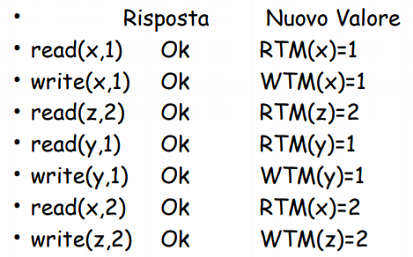
\includegraphics[scale=.65]{img/170.PNG}\end{center}

\chapter{Implementazione dei processi e delle primitive nel modulo sistema}

\section{Premessa: file \emph{include/costanti.h}}
Nel file \emph{sistema.s}, come in altri file di estensione cpp, è incluso con apposita direttiva il file \emph{costanti.h}
\begin{verbatim}
	#include "costanti.h"
\end{verbatim}
esso contiene una serie di costanti, tutte introdotte con \emph{define} per permetterne l'uso sia in C++ sia in Assembler. L'uso di queste costanti sarà evidente da qua fino alla fine della dispensa.

\section{Inizializzazione della \emph{Interrupt Descriptor Table}}
La gestione della \emph{Interrupt Descriptor Table} non è così diversa da quella vista con la libreria \emph{libce}.
\small 
\begin{verbatim}
.global init_idt
init_idt:
    //      indice      routine         dpl
    // gestori eccezioni:
    carica_gate	0       divide_error    LIV_SISTEMA
    carica_gate	1       debug           LIV_SISTEMA
    carica_gate	2       nmi             LIV_SISTEMA
    carica_gate	3       breakpoint      LIV_SISTEMA
    carica_gate	4       overflow        LIV_SISTEMA
    carica_gate	5       bound_re        LIV_SISTEMA
    carica_gate	6       invalid_opcode  LIV_SISTEMA
    carica_gate	7       dev_na          LIV_SISTEMA
    carica_gate	8       double_fault    LIV_SISTEMA
    carica_gate	9       coproc_so       LIV_SISTEMA
    carica_gate	10      invalid_tss     LIV_SISTEMA
    carica_gate	11      segm_fault      LIV_SISTEMA
    carica_gate	12      stack_fault     LIV_SISTEMA
    carica_gate	13      prot_fault      LIV_SISTEMA
    carica_gate	14      page_fault      LIV_SISTEMA
    // ... il tipo 15 è riservato
    carica_gate	16      fp_exc          LIV_SISTEMA
    carica_gate	17      ac_exc          LIV_SISTEMA
    carica_gate	18      mc_exc          LIV_SISTEMA
    carica_gate	19      simd_exc        LIV_SISTEMA
    carica_gate	20      virt_exc        LIV_SISTEMA
    // ... tipi 21-29 riservati
    carica_gate	30      sec_exc         LIV_SISTEMA
    // ... tipo 31 riservato

    // primitive comuni (tipi 0x2-)
    carica_gate	TIPO_A      a_activate_p    LIV_UTENTE
    carica_gate	TIPO_T      a_terminate_p   LIV_UTENTE
    carica_gate	TIPO_SI     a_sem_ini       LIV_UTENTE
    carica_gate	TIPO_W      a_sem_wait      LIV_UTENTE
    carica_gate	TIPO_S      a_sem_signal    LIV_UTENTE
    carica_gate	TIPO_D      a_delay         LIV_UTENTE
    carica_gate	TIPO_L      a_log           LIV_UTENTE
    carica_gate	TIPO_GMI    a_getmeminfo    LIV_UTENTE

    // primitive per il livello I/O (tipi 0x3-) 
    carica_gate	TIPO_APE    a_activate_pe   LIV_SISTEMA
    carica_gate	TIPO_WFI    a_wfi           LIV_SISTEMA
    carica_gate	TIPO_FG     a_fill_gate     LIV_SISTEMA
    carica_gate	TIPO_AB     a_abort_p       LIV_SISTEMA
    carica_gate	TIPO_IOP    a_io_panic      LIV_SISTEMA
    carica_gate	TIPO_TRA    a_trasforma     LIV_SISTEMA
    carica_gate	TIPO_ACC    a_access        LIV_SISTEMA

    // i tipi 0x4- verranno usati per le primitive fornite dal modulo I/O
    // (si veda fill_io_gates() in io.s)
    // i tipi da 0x50 a 0xFE verrano usati per gli handler
    // (si veda load_handler() più avanti)

    // la priorità massima è riservata al driver del timer di sistema
    carica_gate	TIPO_TIMER  driver_td       LIV_SISTEMA

    lidt idt_pointer
    ret
\end{verbatim}
\normalsize 
%\begin{center}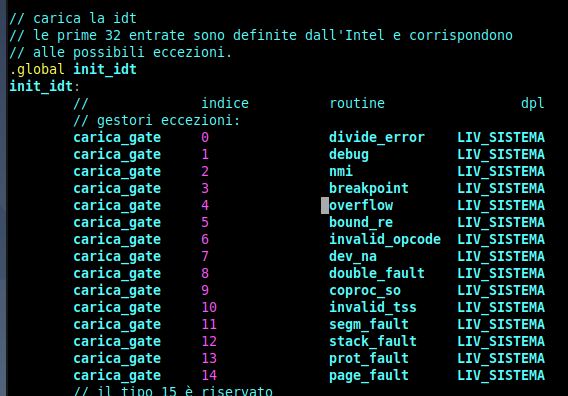
\includegraphics[scale=.75]{img/173.PNG}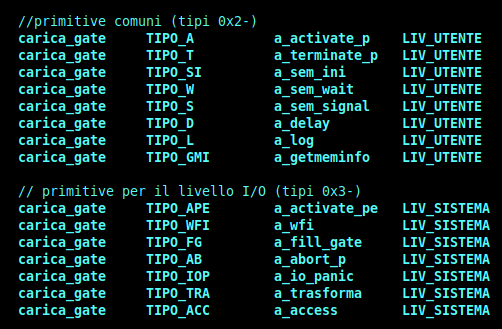
\includegraphics[scale=.75]{img/174.PNG}\end{center}
\begin{itemize}
	\item Abbiamo la \emph{carica$\_$gate}, ma con la possibilità di indicare anche il \emph{Descriptor Privilege Level} del gate (livello considerato solo nel lancio di interruzioni con istruzione INT). 
	\small
	\begin{verbatim}
	// Carica un gate della IDT
	// num: indice (a partire da 0) in IDT del gate da caricare
	// routine: indirizzo della routine da associare al gate
	// dpl: dpl del gate (LIV_SISTEMA o LIV_UTENTE)
	.macro carica_gate num routine dpl
	    movq $\num, %rdi
	    movq $\routine, %rsi
	    movq $\dpl, %rdx
	    xorq %rcx, %rcx
	    call init_gate
	.endm
	\end{verbatim} 
	\normalsize
		\item \textbf{Attenzione}.
	
	Le righe di codice dove usiamo ripetutamente la macro \emph{carica$\_$gate} non sono il luogo dove effettivamente stiamo ponendo la nostra \emph{Interrupt Descriptor Table}. In fondo al file \emph{sistema.s} abbiamo uno spazio destinato a tale scopo
	\small
	\begin{verbatim}
		.bss
		.balign 16
		idt:
		    // spazio per 256 gate
		    // verra' riempita a tempo di esecuzione
		    .space 16*256, 0
	\end{verbatim}
	\normalsize
	La routine \emph{init$\_$gate}, chiamata nella macro, organizza il contenuto di quell'area di memoria ogni volta che viene inserito un gate.
	
	\item \textbf{Istruzione LIDT}.
	
	Con l'istruzione \emph{lidt} andiamo ad aggiornare il registro IDTR 
	\begin{verbatim}
		lidt idt_pointer
	\end{verbatim}
	dove \emph{idt$\_$pointer} è una variabile avente una certa forma:
	\small
	\begin{verbatim}
	.data
	// ...
idt_pointer:
    .word 0xFFF			// limite della IDT (256 entrate)
    .quad idt			// base della IDT
	\end{verbatim}
	\normalsize 
	\begin{itemize}
		\item il \emph{word} ci dicono quanto è grande la \emph{Interrupt Descriptor Table},
		\item il \emph{quad} contiene l'indirizzo della base della IDT (non a caso, \emph{idt}).
	\end{itemize}

		\item Ricordiamo quanto detto con l'APIC
	\small
	\begin{framed}
		\noindent Il livello di priorità è codificato nel tipo. L'identificativo può essere scomposto in due parti:
		\begin{itemize}
			\item la classe di priorità (parte più significativa), e 
			\item la sottopriorità all'interno della classe (parte meno significativa).
		\end{itemize}
		La regola che la APIC segue è di inviare una nuova richiesta di interruzione soltanto se tra quelle pendenti ce n'è una con classe di priorità maggiore della massima classe di priorità che è già stata accettata dal processore. In caso di \emph{ex-aequo} si guarda la sottopriorità.
	\end{framed}
	\normalsize Il primo parametro della \emph{carica$\_$gate} permette di indicare l'identificativo del tipo, dunque la priorità associata: maggiore è il valore numerico, maggiore sarà la priorità. Si osservi a chi viene attribuità la priorità massima: il timer (la cosa non dovrebbe stupirci)!
	\begin{verbatim}
	carica_gate TIPO_TIMER  driver_td       LIV_SISTEMA
	\end{verbatim}
	In \emph{include/costanti.h} sono definite una serie di costanti relative ai tipi dei gate
	\small
	\begin{multicols}{2}
	\begin{verbatim}
		// ( tipi delle primitive
		//   ( comuni
		#define TIPO_A			0x20	// activate_p
		#define TIPO_T			0x21	// terminate_p
		#define TIPO_SI			0x22	// sem_ini
		#define TIPO_W			0x23	// sem_wait
		#define TIPO_S			0x24	// sem_signal
		#define TIPO_D			0x25	// delay
		#define TIPO_L			0x26	// log
		#define TIPO_GMI		0x27	// getmeminfo (debug)
		//   )
		
		//   ( riservate per il modulo I/O
		#define TIPO_APE		0x30	// activate_pe
	\end{verbatim}
	\columnbreak 
	\begin{verbatim}
		#define TIPO_WFI		0x31	// wfi
		#define TIPO_FG			0x32	// fill_gate
		#define TIPO_AB			0x33	// abort_p
		#define TIPO_IOP		0x34	// io_panic
		#define TIPO_TRA		0x35	// trasforma
		#define TIPO_ACC		0x36	// access
		//   )
		
		// ...
		
		// tipo del driver del timer (priorità  massima)
		#define TIPO_TIMER		0xFF
	\end{verbatim}
\end{multicols}
	\normalsize
	\item Possiamo classificare i gate già caricati in:
	\begin{itemize}
		\item eccezioni (dal gate 0 al gate 31, possibili eccezioni definite dalla Intel);
		\item primitive comuni (eseguibili a livello utente);
		\item primitive per il livello I/O (primitive che saranno utilizzate nel modulo I/O).
	\end{itemize}
	Altri gate saranno caricati più avanti, nel modulo I/O:
	\small 
	\begin{verbatim}
	// i tipi 0x4- verranno usati per le primitive fornite dal modulo I/O
	// (si veda fill_io_gates() in io.s)
	// i tipi da 0x50 a 0xFE verrano usati per gli handler
	// (si veda load_handler() più avanti)
	\end{verbatim}
	\normalsize 
	\item \textbf{Ma non è limitante usare un gate per ogni primitiva?} 
	
	Solitamente per tutte le primitive si usa un unico gate: la primitiva chiamata viene decisa sulla base di un valore posto in un registro (RAX, usa quel numero per accedere a un array di puntatori). In questo modo non siamo più limitati dall'hardware nel numero di primitive! Noi non faremo così: per quello che dobbiamo fare non ci serve un numero spropositato di primitive.
\end{itemize}

%\begin{center}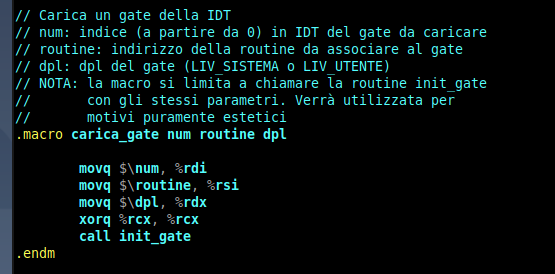
\includegraphics[scale=.8]{img/172.PNG}\end{center}

\section{Inizializzazione della \emph{Global Descriptor Table}}
Facciamo cose molto simili anche per la \emph{Global Descriptor Table}, che come già detto dobbiamo utilizzare (non come concepito all'inizio) per le modalità sistema e utente. All'interno della GDT troviamo anche il segmento TSS, che ci serve per gestire il cambio della pila.
\small 
\begin{verbatim}
.balign 8
.global gdt
gdt:
    .quad 0		    //segmento nullo
code_sys_seg:
    .word 0b0           //limit[15:0]   not used
    .word 0b0           //base[15:0]    not used
    .byte 0b0           //base[23:16]   not used
    .byte 0b10011010    //P|DPL|1|1|C|R|A|  DPL=00=sistema
    .byte 0b00100000    //G|D|L|-|-------|  L=1 long mode
    .byte 0b0           //base[31:24]   not used
code_usr_seg:
    .word 0b0           //limit[15:0]   not used
    .word 0b0           //base[15:0]    not used
    .byte 0b0           //base[23:16]   not used
    .byte 0b11111010    //P|DPL|1|1|C|R|A|  DPL=11=utente
    .byte 0b00100000    //G|D|L|-|-------|  L=1 long mode
    .byte 0b0           //base[31:24]   not used
data_usr_seg:
    .word 0b0           //limit[15:0]   not used
    .word 0b0           //base[15:0]    not used
    .byte 0b0           //base[23:16]   not used
    .byte 0b11110010    //P|DPL|1|0|E|W|A|  DPL=11=utente
    .byte 0b00000000    //G|D|-|-|-------|
    .byte 0b0           //base[31:24]   not used
tss_seg:
    .space 16, 0	    // riempito da init_gdt
end_gdt:

tss:
    .long 0
    .global tss_punt_nucleo
tss_punt_nucleo:
    .quad 0
    .space 11 * 8, 0
    .word 0
    .word tss_end - tss - 1
tss_end:
\end{verbatim}
\normalsize 
Ci servono, come già anticipato:
\begin{itemize}
	\item un'entrata della GDT per gestire il passaggio da modalità utente a modalità sistema o per rimanere in modalità sistema;
	\item un'entrata della GDT per attraversare il gate e rimanere in modalità utente;
	\item il \emph{Task State Segment} per gestire il cambio della pila (nei modi già spiegati quando abbiamo affrontato l'implementazione della protezione nel processore Intel), di esso ci interessa solo la riga \emph{tss$\_$punt$\_$nucleo} (un \emph{quad} dove metteremo l'indirizzo della pila sistema ogni volta che cambiamo processo).
\end{itemize}
A un certo punto, da \emph{sistema.cpp}, verrà chiamata la funzione \emph{gdt$\_$init} (il cui codice si trova in \emph{sistema.s}). Non ci interessa il codice (Lettieri non l'ha neanche guardato), dobbiamo solo ricordarci che:
\begin{itemize}
	\item inizializza il contenuto del \emph{Task State Segment} (non è possibile farlo staticamente, nelle righe precedenti abbiamo solo preparato l'area di memoria);
	\item esegue la seguente istruzione
	\begin{verbatim}
	lgdt gdt_pointer
	\end{verbatim}
	dove \emph{gdt$\_$pointer} è un'area di ottanta byte con sintassi simile alla \emph{idt$\_$pointer}
	\begin{verbatim}
	.data
	gdt_pointer:
	    .word end_gdt - gdt // limite della GDT
	    .quad gdt
	\end{verbatim}
\end{itemize}
\small 
\normalsize 
%\begin{center}
\includegraphics[scale=.8]{img/177.PNG}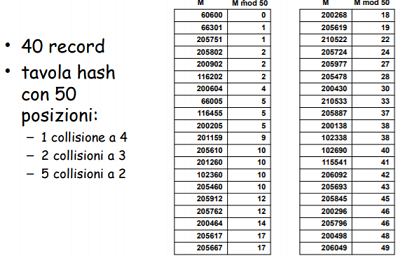
\includegraphics[scale=.8]{img/178.PNG}\end{center}



\section{Processo \emph{dummy} e shutdown con \emph{end$\_$program}}
Nella funzione \emph{main} di \emph{sistema.cpp} viene creato il cosiddetto \emph{processo dummy}.
\small 
\begin{verbatim}
// creazione del processo dummy
dummy_id = crea_dummy();
if(dummy_id == 0xFFFFFFFF)
    goto error;
flog(LOG_INFO, "Creato il processo dummy (id = %d)", dummy_id);
\end{verbatim}
\normalsize 
Esso permette di evitare il caso particolare in cui i processi sono tutti bloccati e non c'è altro da fare: risolvo la cosa con un processo a bassa priorità, dunque lo schedulatore trova sempre qualcosa da fare.
\subsection{Funzioni \emph{dummy} e \emph{crea$\_$dummy}}
\small
\begin{verbatim}
extern "C" void end_program();
void dummy(natq i) {
    while(processi)
        ;
    end_program();
}

natl crea_dummy() {
    des_proc* di = crea_processo(dummy, 0, DUMMY_PRIORITY, LIV_SISTEMA, true);
    if(di == 0) {
        flog(LOG_ERR, "Impossibile creare il processo dummy");
        return 0xFFFFFFFF;
    }
    inserimento_lista(pronti, di);
    return di->id;
}
\end{verbatim}
\normalsize 
%\begin{center}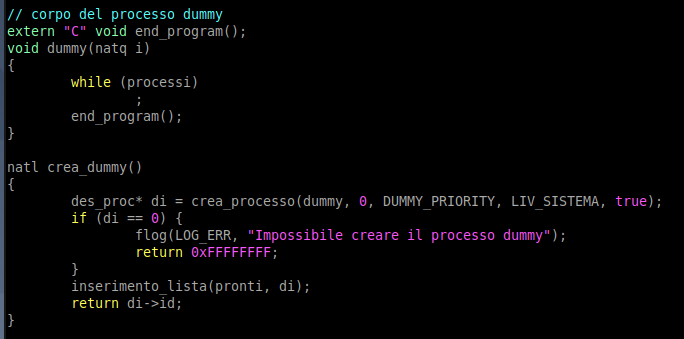
\includegraphics[scale=.9]{img/182.PNG}	
%	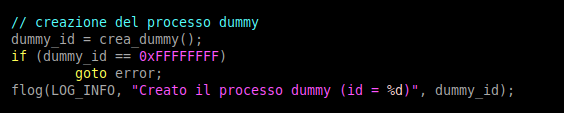
\includegraphics{img/181.PNG}\end{center}
La funzione \emph{dummy} si limita a guardare in continuazione la variabile \emph{processi}, che consiste nel numero di processi. Gira li finché il numero di processi attivi non sarà nullo\footnote{Ovviamente si tenga conto del passaggio a processi con priorità maggiore, cosa che avviene quando almeno un processo non è occupato.}.

\subsection{Funzione \emph{end$\_$program}} 
La funzione \emph{end$\_$program} verrà eseguita solo se non si hanno processi da eseguire, quindi se usciamo dal ciclo presente nella funzione \emph{dummy}. Il trucco consiste nel provocare un'eccezione di tipo \emph{abort}. Mette nella IDT un puntatore nullo (usando la LIDT) e lancia un'interruzione (con INT): nella IDT viene caricato un puntatore nullo, dunque trova l'indirizzo $0$ (non valido) e lancia un'eccezione di \emph{gate non valido}, anche in quel caso non trova l'indirizzo e lancia una terza eccezione che provoca \emph{abort} e quindi lo spegnimento.
\begin{verbatim}
    .global end_program
end_program: 
    lidt triple_fault_idt 
    int $1

// ...
   
.data 
triple_fault_idt:
    .word 0
\end{verbatim}
 %\begin{center}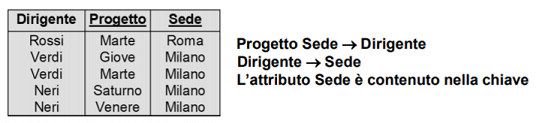
\includegraphics{img/183.PNG}\end{center}



\section{Strutture dati per la gestione dei processi}
\subsection{Descrittore di processo}
In \emph{sistema.cpp} abbiamo il descrittore di processo, già ampiamente descritto. 
\small 
\begin{verbatim}	
const int N_REG = 16;
struct des_proc {
    natw id;
    natw livello;
    natl precedenza;
    vaddr punt_nucleo; /* Puntatore a pila sistema */
    natq contesto[N_REG];
    paddr cr3;
		
    des_proc *puntatore;
};
\end{verbatim}
\normalsize 
\subsection{Array dei processi}Tutti i descrittori di processo sono raccolti in un'array
\begin{verbatim}
des_proc* proc_table[MAX_PROC];
\end{verbatim}
dove \emph{MAX$\_$PROC} è una costante posta in \emph{include/costanti.h}. 
\begin{verbatim}
#define MAX_PROC        1024UL
\end{verbatim}
\subsection{Indici dei registri nell'array \emph{contesto}} Per quanto riguarda l'array \emph{contesto} si consideri l'\emph{enum} contenente i vari indici dei vari registri all'interno dell'array \emph{contesto}.
\begin{verbatim}
	enum { I_RAX, I_RCX, I_RDX, I_RBX, I_RSP, I_RBP, I_RSI, I_RDI, I_R8, I_R9, I_R10, 
		I_R11, I_R12, I_R13, I_R14, I_R15};
\end{verbatim}
quando andremo a manipolare i registri del contesto utilizzeremo queste costanti (non serve quindi conoscere l'indice preciso). \paragraph{Esempio}
\begin{verbatim}
	esecuzione->contesto[I_RAX] = true;
\end{verbatim}

\subsection{Puntatori}
Nel codice abbiamo questi due puntatori
\begin{verbatim}
des_proc *esecuzione; 
des_proc *pronti;
\end{verbatim}
\begin{itemize}
	\item \textbf{esecuzione} consiste nel puntatore all'unico processo in esecuzione nel processore.
	\item \textbf{pronti} è il puntatore alla testa di una lista di processi in attesa. La lista è costruita utilizzando, nella struttura \emph{des$\_$proc}, il puntatore \emph{puntatore}.
\end{itemize}

\subsection{Conteggio del numero di processi}
%Usando l'array precedente posso capire se un certo ID è già stato utilizzato: al momento della creazione di un processo scorro l'array finchè non ho un'entrata con \emph{null pointer}.
Poco dopo è definita la variabile \emph{processi}, che come già anticipato conteggia il numero di processi attivi.
\begin{verbatim}
	volatile natl processi;
\end{verbatim}
Viene posta \emph{volatile} poichè utilizzata nella funzione \emph{dummy}.

\section{Funzioni per la manipolazione delle liste}
In \emph{sistema.cpp} sono presenti delle funzioni che permettono di manipolare le liste. Ricordiamo che le liste relative ai processi sono ordinate esclusivamente in base alla precedenza. 
\subsection{Funzione \emph{inserimento$\_$lista}}
\small
\begin{verbatim}
void inserimento_lista(des_proc* &p_lista, des_proc* p_elem) {
    // inserimento in una lista semplice ordinata
    // (tecnica dei due puntatori)
    des_proc *pp, *prevp;
    
    pp = p_lista;
    prevp = nullptr;
    while(pp && pp->precedenza >= p_elem->precedenza) {
        prevp = pp;
        pp = pp->puntatore;
    }

    p_elem->puntatore = pp;
    
    if(prevp)
        prevp->puntatore = p_elem;
    else
        p_lista = p_elem;
}
\end{verbatim}
\normalsize 
\begin{itemize}
	\item La funzione \emph{inserimento$\_$lista} permette l'inserimento in una qualunque lista di un elemento \emph{des$\_$proc}. L'inserimento dell'elemento \emph{p$\_$elem} si basa sulle precedenze (chi ha precedenza più alta sta in cima alla lista), con logica FIFO (a parità di precedenza vince l'elemento inserito per primo nella lista).
	\item Il parametro di ingresso \emph{p$\_$lista} è il puntatore alla lista da manipolare (con riferimento, potrei porre un elemento in cima alla lista). 
	\item Il parametro di ingresso \emph{p$\_$elem} è il puntatore all'elemento da inserire nella lista.
	\item Il codice è simile, se non identico, alla funzione studiata a \emph{Fondamenti di programmazione} per l'inserimento di un elemento in una lista: 
	\begin{itemize}
		\item scorro la lista finché non trovo il punto dove il processo deve essere inserito;
		\item modifico \emph{puntatore} dell'elemento precedente e imposto \emph{puntatore} del processo appena inserito.
	\end{itemize}
\end{itemize}
\subsection{Funzione \emph{rimozione$\_$lista}}
\small
\begin{verbatim}
des_proc* rimozione_lista(des_proc* &p_lista) {
    // estrazione della testa
    des_proc *p_elem = p_lista // nullptr se la lista e' vuota
    
    if(p_lista)
        p_lista = p_lista->puntatore;
        
    if(p_elem)
        p_elem->puntatore = nullptr;
        
    return p_elem;
}
\end{verbatim}
\normalsize
\begin{itemize}
	\item La funzione \emph{rimozione$\_$lista} permette la rimozione della testa di una qualunque lista di elementi \emph{des$\_$proc}.
	\item Il parametro di ingresso \emph{p$\_$lista} è il puntatore alla lista (con riferimento, visto che rimuoviamo la testa).
	\item Pongo nel puntatore \emph{p$\_$elem} l'indirizzo della testa.
	\item Se nella lista puntata da \emph{p$\_$lista} sono presenti elementi (prima di procedere all'estrazione) modifico il puntatore \emph{p$\_$lista} rendendo il secondo elemento la nuova testa.
	\item Se l'elemento estratto non è nullo modifico il suo \emph{puntatore} ponendolo a null (lo abbiamo scollegato dalla lista, non ha senso mantenere un collegamento).
	\item Restituisco l'indirizzo della testa estratta (\emph{p$\_$elem}).
\end{itemize}

\subsection{Funzione \emph{inspronti} per la lista \emph{pronti}}
\small
\begin{verbatim}
extern "C" void inspronti() {
    esecuzione->puntatore = pronti;
    pronti = esecuzione;
}
\end{verbatim}
\normalsize 
La funzione \emph{inspronti} inserisce il processo attualmente in esecuzione in testa alla lista \emph{pronti}. Si consideri che:
\begin{itemize}
	\item se abbiamo lavorato bene inseriremo in testa il processo con priorità maggiore;
	\item abbiamo aggiornato la lista \emph{pronti}, \textbf{ma non abbiamo modificato \emph{esecuzione}} (il processo posto in \emph{esecuzione} è sempre quello attualmente in esecuzione).
\end{itemize}

\subsection{Funzione \emph{schedulatore} per la lista \emph{pronti}}
\[\boxed{\text{\textbf{Promemoria}. La schedulazione è il passaggio di un processo da \emph{pronto} a \emph{esecuzione}}}\]
La funzione \emph{schedulatore} comporterà il passaggio di un processo (quello con priorità maggiore) dallo stato \emph{pronto} a \emph{esecuzione}. Le cose da fare sono due:
\begin{enumerate}
	\item estrarre la testa dalla coda \emph{pronti} (in testa abbiamo, secondo logica FIFO, il processo con priorità maggiore);
	\item fare puntare il processo appena estratto dal puntatore \emph{esecuzione}.
\end{enumerate}
Grazie alla funzione \emph{rimozione$\_$lista} il codice della funzione \emph{schedulatore} è molto breve.
\small
\begin{verbatim}
extern "C" void schedulatore(void) {
    esecuzione = rimozione_lista(pronti);
}
\end{verbatim}
\normalsize
\paragraph{Attenzione} La funzione sceglie soltanto il processo che dovrà andare in esecuzione quando è finita la primitiva! \textbf{Non si ha il cambio di processo nel momento in cui chiamiamo schedulatore}. \textit{Se pensate che scrivere dentro una variabile basti per cambiare il processo allora avete le idee un po' confuse (cit.)}.

\section{Funzioni \emph{salva$\_$stato} e \emph{carica$\_$stato}}

Nel file \emph{sistema.s} abbiamo due funzioni familiari: \emph{salva$\_$stato} e \emph{carica$\_$stato}. Nulla di strano, solo un qualcosa di intricato.

\subsection{Premessa: offset}
Sono definite in Assembler una serie di costanti per gestire gli offset:
\small 
\begin{verbatim}
	// offset dei vari registri all'interno di des_proc
	.set PUNT_NUCLEO, 8
	.set CTX, 16
	.set RAX, CTX+0
	.set RCX, CTX+8
	.set RDX, CTX+16
	.set RBX, CTX+24
	.set RSP, CTX+32
	.set RBP, CTX+40
	.set RSI, CTX+48
	.set RDI, CTX+56
	.set R8,  CTX+64
	.set R9,  CTX+72
	.set R10, CTX+80
	.set R11, CTX+88
	.set R12, CTX+96
	.set R13, CTX+104
	.set R14, CTX+112
	.set R15, CTX+120
	.set CR3, CTX+128
\end{verbatim}
\normalsize 
In entrambe le funzioni gli offset vengono utilizzati rispetto al registro RBX, dove abbiamo posto \emph{esecuzione} (quindi gli offset sono costruiti tenendo conto della struttura di \emph{des$\_$proc})
\begin{verbatim}
movq esecuzione, %rbx
\end{verbatim}
\subsection{salva$\_$stato}	
\small 
\begin{verbatim}
// copia lo stato dei registri generali nel des_proc del processo puntato da
// esecuzione.  Nessun registro viene sporcato.

salva_stato:
    // salviamo lo stato di un paio di registri in modo da poterli
    // temporaneamente riutilizzare. In particolare, useremo %rax come
    // registro di lavoro e %rbx come puntatore al des_proc.
    pushq %rbx
    pushq %rax

    movq esecuzione, %rbx

    // copiamo per primo il vecchio valore di %rax
    movq (%rsp), %rax
    movq %rax, RAX(%rbx)
    // usiamo %rax come appoggio per copiare il vecchio %rbx
    movq 8(%rsp), %rax
    movq %rax, RBX(%rbx)
    // copiamo gli altri registri
    movq %rcx, RCX(%rbx)
    movq %rdx, RDX(%rbx)
    // salviamo il valore che %rsp aveva prima della chiamata a salva stato
    // (valore corrente meno gli 8 byte che contengono l'indirizzo di
    // ritorno e i 16 byte dovuti alle due push che abbiamo fatto all'inizio)
    movq %rsp, %rax
    addq $24, %rax
    movq %rax, RSP(%rbx)
    movq %rbp, RBP(%rbx)
    movq %rsi, RSI(%rbx)
    movq %rdi, RDI(%rbx)
    movq %r8,  R8 (%rbx)
    movq %r9,  R9 (%rbx)
    movq %r10, R10(%rbx)
    movq %r11, R11(%rbx)
    movq %r12, R12(%rbx)
    movq %r13, R13(%rbx)
    movq %r14, R14(%rbx)
    movq %r15, R15(%rbx)

    popq %rax
    popq %rbx

    ret
\end{verbatim}
\normalsize 
\begin{itemize}
\item La funzione deve essere chiamata subito dopo essere entrati nel modulo sistema, per qualunque motivo. Deve memorizzare lo stato di tutti i registri nel momento in cui è stata chiamata. 
	\item I registri che utilizziamo per svolgere le nostre operazioni sono RAX ed RBX. Il primo è utilizzato come registro di lavoro (cioè per fare passi intermedi), mentre RBX lo usiamo per puntare al descrittore di processo corrente (posto nella variabile globale \emph{esecuzione}). Per fare queste cose poniamo in pila il contenuto vecchio di RAX ed RBX
	\begin{verbatim}
		pushq %rbx
		pushq %rax
	\end{verbatim}
	 %\begin{center}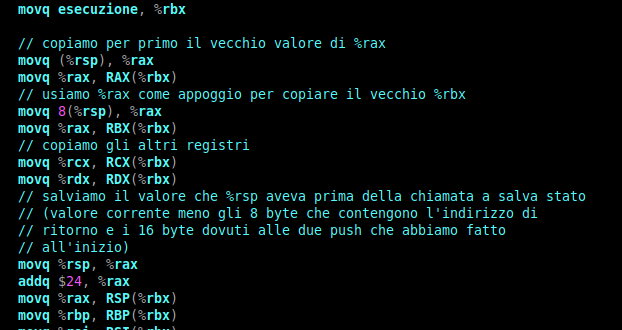
\includegraphics[scale=.9]{img/184.PNG}\end{center}
		\item Pongo in rbx il contenuto della variabile globale \emph{esecuzione} 
		\begin{verbatim}
			movq esecuzione, %rbx
		\end{verbatim}
		\item Pongo nel \emph{contesto} il contenuto di RAX
		\item Pongo nel \emph{contesto} il contenuto di RBX, utilizzando RAX come registro di lavoro (ho bisogno di un registro dove spostare il mio risultato intermedio, per forza).
		\item Segue una sfilata di costanti attraverso cui indichiamo i relativi offset e spostiamo in \emph{contesto} il contenuto dei registri rimanenti.
		\item Per porre il valore vecchio di RSP dobbiamo ricordarci che abbiamo eseguito una chiamata di funzione e due push, dunque RSP è già stato spostato rispetto all'inizio. Segue
		\begin{verbatim}
			movq %rsp, %rax
			addq $24, %rax
		\end{verbatim} Useremo il valore vecchio calcolato nella IRETQ per la lettura della pila sistema.
		\item Esegiamo le due pop consuete dopo aver finito di utilizzare i registri RAX ed RBX
		\begin{verbatim}
			pop %rax
			pop %rbx
		\end{verbatim}
	\end{itemize}
	
\subsection{carica$\_$stato}
\small 
\begin{verbatim}
// carica nei registri del processore lo stato contenuto nel des_proc del
// processo puntato da esecuzione.  Questa funzione sporca tutti i registri.
carica_stato:
    movq esecuzione, %rbx

    popq %rcx   //ind di ritorno, va messo nella nuova pila

    // nuovo valore per cr3
    movq CR3(%rbx), %r10
    movq %cr3, %rax
    cmpq %rax, %r10
    je 1f			// evitiamo di invalidare il TLB
    // se cr3 non cambia
    movq %r10, %rax
    movq %rax, %cr3		// il TLB viene invalidato
1:
    // anche se abbiamo cambiato cr3 siamo sicuri che l'esecuzione prosegue
    // da qui, perché ci troviamo dentro la finestra FM che è comune a
    // tutti i processi
    movq RSP(%rbx), %rsp    //cambiamo pila
    pushq %rcx              //rimettiamo l'indirizzo di ritorno

    // se il processo precedente era terminato o abortito la sua pila
    // sistema non era stata distrutta, in modo da permettere a noi di
    // continuare ad usarla. Ora che abbiamo cambiato pila possiamo
    // disfarci della precedente.
    cmpq $0, ultimo_terminato
    je 1f
    call distruggi_pila_precedente
1:
    // aggiorniamo il puntatore alla pila sistema usata dal meccanismo
    // delle interruzioni
    movq PUNT_NUCLEO(%rbx), %rcx
    movq %rcx, tss_punt_nucleo

    movq RCX(%rbx), %rcx
    movq RDI(%rbx), %rdi
    movq RSI(%rbx), %rsi
    movq RBP(%rbx), %rbp
    movq RDX(%rbx), %rdx
    movq RAX(%rbx), %rax
    movq R8(%rbx), %r8
    movq R9(%rbx), %r9
    movq R10(%rbx), %r10
    movq R11(%rbx), %r11
    movq R12(%rbx), %r12
    movq R13(%rbx), %r13
    movq R14(%rbx), %r14
    movq R15(%rbx), %r15
    movq RBX(%rbx), %rbx

    retq
\end{verbatim}
\normalsize 
	%\begin{center}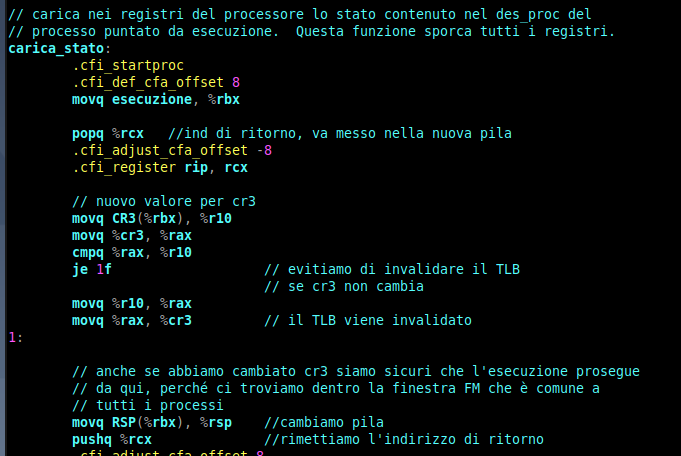
\includegraphics[scale=.9]{img/185.PNG}\end{center}
	\begin{itemize}
		\item La funzione ha un problema: è stata chiamata, il suo indirizzo di ritorno è stato messo nella pila corrente, se il valore di \emph{esecuzione} è stato modificato a un certo punto tra tutti i registri caricherà anche rsp. La pila punterà da un'altra parte, ma l'indirizzo di ritorno si trova nella vecchia pila. Dobbiamo complicarci un attimo la vita per spostare l'indirizzo di ritorno dalla pila vecchia a quella nuova.
		\item Verifico se il processo precedente è stato terminato o abortito. In quel caso la pila sistema può essere distrutta (se terminiamo un processo allora la pila sistema relativa al processo non sarà più utilizzata).
		\item Pongo in RBX, come prima, l'indirizzo al descrittore di processo
		\begin{verbatim}
			movq esecuzione, %rbx
		\end{verbatim}
		\item Metto in RCX l'indirizzo di ritorno, lo levo dalla pila precedente.
		\item Il registro CR3 viene affrontato nel capitolo sulla paginazione.
		\item Modifico RSP mettendo il valore relativo alla nuova pila.
		\item Eseguo la POP per inserire nella nuova pila l'indirizzo di ritorno
		\begin{verbatim}
			pushq %rcx
		\end{verbatim}
		\item A questo punto carico tutti i registri. 
		\item In più, aggiorno \emph{tss$\_$punt$\_$nucleo}  nel TSS (ricordare quanto deciso sull'uso del TSS - univoco per tutti i processi, con necessità di modificare ogni volta il puntatore alla pila sistema nel TSS stesso).
		%\begin{center}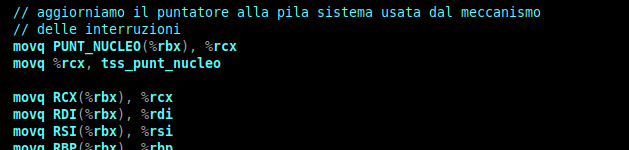
\includegraphics[scale=.9]{img/186.PNG}\end{center}
	\end{itemize}




\section{Primitive}
Il codice di una primitiva è sempre strutturato in due parti:
\begin{itemize}
	\item una parte in Assembler dove eseguiamo all'inizio la \emph{salva$\_$stato} e alla fine la \emph{carica$\_$stato};
	\item una routine scritta in C++, chiamata tra le due funzioni appena citate.
\end{itemize}
Il codice vero e proprio della primitiva è posto nella routine.
\subsection{Funzione di utilità \emph{liv$\_$chiamante}}
\[\boxed{\text{Funziona solo se è stata chiamata la \emph{salva$\_$stato}}}\]
La funzione \emph{liv$\_$chiamante} restituisce il livello di privilegio a cui si trovava il processore nel momento in cui è stata invocata la primitiva.
\small 
\begin{verbatim}
int liv_chiamante() {
    // salva_stato ha salvato il puntatore alla pila sistema
    // subito dopo l'invocazione della INT
    natq *pila = reinterpret_cast<natq*>(esecuzione->contesto[I_RSP]);
    
    // la seconda parola dalla cima della pila contiene il livello
    // di privilegio che aveva il processore prima della INT
    return pila[1] == SEL_CODICE_SISTEMA ? LIV_SISTEMA : LIV_UTENTE;
}
\end{verbatim}
\normalsize
\begin{itemize}
	\item La funzione recupera dal registro RSP nel contesto la pila.
	\item Dalla seconda \emph{quadword} nella pila (indice $1$) viene recuperato il \emph{Current Privilege Level}.
	\item Abbiamo utilizzato alcune costanti poste in \emph{include/costanti.h}
	\begin{verbatim}
	#define SEL_CODICE_SISTEMA        0x8
	#define LIV_UTENTE        3
	#define LIV_SISTEMA        0
	\end{verbatim}
\end{itemize}
\paragraph{Perchè non usare \emph{punt$\_$nucleo}?} L'indirizzo in \emph{punt$\_$nucleo} è quello della base della pila. Noi non sappiamo quale sia la distanza tra la base e la \emph{quadword} che ci interessa.
\subsection{Analisi della struttura della primitiva \emph{activate$\_$p}}
\subsubsection{Parte Assembler}
\small 
\begin{verbatim}
    .extern c_activate_p
a_activate_p:
    call salva_stato
    call c_activate_p
    call carica_stato
    iretq
\end{verbatim}
\normalsize 
Abbiamo il solito incapsulamento con \emph{salva$\_$stato} (eseguita prima della parte C++ della primitiva) e \emph{carica$\_$stato} (eseguita dopo la parte C++ della primitiva). Nulla di particolare rispetto a quanto già detto.
\subsubsection{Parte C++}
\small 
\begin{verbatim}
extern "C" void c_activate_p(void f(natq), natq a, natl prio, natl liv) {
    des_proc *p;			// des_proc per il nuovo processo
    natl id = 0xFFFFFFFF;		// id da restituire in caso di fallimento
	
    // non possiamo accettare una priorita'  minore di quella di dummy
    // o maggiore di quella del processo chiamante
    if (prio < MIN_PRIORITY || prio > esecuzione->precedenza) {
        flog(LOG_WARN, "priorita' non valida: %d", prio);
        c_abort_p();
        return;
    }
	
    // controlliamo che 'liv' contenga un valore ammesso
    // [segnalazione di E. D'Urso]
    if (liv != LIV_UTENTE && liv != LIV_SISTEMA) {
        flog(LOG_WARN, "livello non valido: %d", liv);
        c_abort_p();
        return;
    }
	
    // non possiamo creare un processo di livello sistema mentre
    // siamo a livello utente
    if (liv == LIV_SISTEMA && liv_chiamante() == LIV_UTENTE) {
        flog(LOG_WARN, "errore di protezione");
        c_abort_p();
        return;
    }
	
    // accorpiamo le parti comuni tra c_activate_p e c_activate_pe
    // nella funzione ausiliare crea_processo
    p = crea_processo(f, a, prio, liv, (liv == LIV_UTENTE));
	
    if (p != nullptr) {
        inserimento_lista(pronti, p);
        processi++;
        id = p->id;			// id del processo creato
        // (allocato da crea_processo)
        flog(LOG_INFO, "proc=%d entry=%p(%d) prio=%d liv=%d", id, f, a, prio, liv);
    }
	
    esecuzione->contesto[I_RAX] = id;
}
\end{verbatim}
\normalsize 
\begin{itemize}
	\item La \emph{c$\_$activate$\_$p} è l'implementazione vera e propria della primitiva \emph{activate$\_$p}, scritta in C++. 
	\begin{itemize}
		\item Si osservi il primo parametro di ingresso
		\begin{verbatim}
			void f(natq)
		\end{verbatim}
		esso è un puntatore a funzione, una funzione avente come unico parametro in ingresso \emph{natq}. Porremo questo valore attraverso il secondo parametro di ingresso.
		\item Vengono posti una serie di controlli per verificare la validità dei parametri in ingresso
		\begin{itemize}
			\item Verifico se la priorità posta dall'utente col parametro \emph{prio} sia minore della priorità minima e/o maggiore della priorità del processo attualmente in esecuzione. La prima cosa deve essere evitata, visto che non posso avere processi con priorità più bassa di \emph{dummy}, la seconda è una forma di semplificazione.
			\item Verifico se il livello posto con \emph{liv} sia un valore valido.
			\item Verifico che non venga richiesta l'attivazione di un processo a livello sistema da parte di un chiamante a livello utente (abbiamo già detto che possiamo creare processi di questo livello solo a livello sistema). Il livello del chiamante viene ottenuto con la funzione di utilità \emph{liv$\_$chiamante}.
		\end{itemize}
	\end{itemize}
	\item Alla fine creo effettivamente il processo con un'altra funzione, che possiamo ignorare (cit.)
	\begin{verbatim}
		p = crea_processo(f, a, prio, liv, (liv == LIV_UTENTE));
	\end{verbatim}
	Se tutto va bene la funzione mi restituisce l'ID univoco del processo creato.
	\item Incremento \emph{processo}, variabile globale che conteggia il numero di processi esistenti. Stampo un avviso con i dati di base relativi al processo.
	\begin{framed}
	\item La primitiva deve restituire al chiamante l'id del processo chiamato. Questo è stato allocato dalla \emph{crea$\_$processo}, che lo ha posto nel descrittore di processo. Per restituirlo stiamo facendo in modo diverso da una \emph{return}
	\begin{verbatim}
		esecuzione->contesto[I_RAX] = id;
	\end{verbatim}
	\textbf{Come mai?} 
	
	Perchè la \emph{carica$\_$stato} sovrascrive quanto posto se poniamo direttamente il valore in RAX. Il valore di \emph{esecuzione}, non è stato modificato, dunque indica il processo che ha invocato l'\emph{activate$\_$p}. Ricordarsi la funzione del registro RAX nella traduzione C++-Assembler.
	\end{framed}
\end{itemize}

\subsubsection{Invocazione della primitiva da parte di un utente}
Poniamoci un'ulteriore domanda...
\paragraph{Come fa l'utente a chiamare la primitiva?} Noi abbiamo parlato solo di funzioni che hanno prefisso \emph{a} (Assembler) o \emph{c} (C++), ma l'utente chiama cose senza prefissi. Sappiamo che dobbiamo eseguire un'istruzione INT. Noi nel codice poniamo una cosa del genere
\begin{verbatim}
	activate_p(f, 10, 10, LIV_UTENTE);
\end{verbatim}
dal punto di vista del C++ stiamo chiamando una normale funzione C++. Vediamo il codice che si cela dietro
\small 
\begin{verbatim}
    .global activate_p
activate_p:
    int $TIPO_A
    ret
\end{verbatim}
\normalsize 
%\begin{center}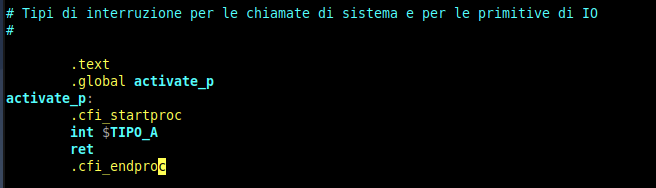
\includegraphics[scale=.76]{img/190.PNG}\end{center}
Abbiamo una \textbf{funzione di appoggio} scritta in Assembler (per forza, non posso eseguire la INT in C++). L'identificativo del tipo dell'interruzione relativa alla primitiva deve essere noto: poniamo per comodità le costanti \emph{TIPO$\_$x} nel file \emph{include/costanti.h}.

\paragraph{Effetto dell'esecuzione di INT?} Lancio di \emph{a$\_$activate$\_$p}. I parametri posti in ingresso non sono stati modificati e possono essere usati.

\subsection{Esempio di primitiva creata da noi: \emph{getprec}}
Proviamo a creare una nostra primitiva, cosa che tipicamente si fa negli esercizi di esame.
\paragraph{Cosa dobbiamo fare?} Facciamo una primitiva con cui un processo può farsi dire dal sistema qual è la sua precedenza.
\begin{itemize}
	\item \textbf{Assegnazione di un identificativo al tipo di interruzione}. 
	
	La prima cosa da fare è assegnare un numero. Vado in \emph{costanti.h} e definisco una nuova costante con la direttiva define
	\begin{verbatim}
		#define TIPO_GETPREC     0x28
	\end{verbatim}
	Ovviamente poniamo un numero che non è ancora utilizzato.
	
	\item \textbf{Aggiungo un gate nell'IDT}.
	
	Modifico il codice relativo al caricamento dell'IDT in \emph{sistema.s}. Carico un gate 
	\begin{verbatim}
		carica_gate     TIPO_GETPREC     a_getprec     LIV_UTENTE
	\end{verbatim}
	chiaramente devo mettere \emph{LIV$\_$UTENTE}, altrimenti non potremo chiamare la primitiva.
	
	\item \textbf{Funzione di "incapsulamento" con \emph{salva} e \emph{carica} stato}. 
	
	In \emph{utenti.s} scriviamo \emph{a$\_$getprec}. La struttura è sempre la stessa
	\begin{verbatim}
		a_getprec:
		    call salva_stato
		    call c_getprec
		    call carica_stato
		    iretq
	\end{verbatim}
	
	\item \textbf{Implementazione concreta della primitiva}. 
	
	Scriviamo il succo della primitiva in C++ (cioè scriviamo la funzione \emph{c$\_$getprec} chiamata tra la \emph{salva$\_$stato} e la \emph{carica$\_$stato}).
	\begin{verbatim}
		extern "C" void c_getprec() {
			    esecuzione->contesto[I_RAX] = esecuzione->precedenza;
		}
	\end{verbatim}
	Chiaramente una cosa del genere può essere fatta solo in modalità sistema, unico modo per accedere ad \emph{esecuzione} e a ciò che punta \emph{esecuzione} stesso.
	\item \textbf{Funzione di appoggio}. 
	
	No, l'utente non può ancora chiamare la primitiva in C++: manca la funzione di appoggio che esegue la INT. Andiamo in \emph{include/sys.h}, dove dichiariamo la nostra primitiva
	\begin{verbatim}
		extern "C" natl getprec();
	\end{verbatim}
	Poi, in \emph{utente/utente.s}, scriviamo quanto segue
	\begin{verbatim}
		getprec:    
		    int $TIPO_GETPREC
		    ret
	\end{verbatim}
	Adesso abbiamo davvero finito.
\end{itemize}
\paragraph{Esempio di chiamata della primitiva}
\begin{verbatim}
	#include <all.h>
	void f(natq a) {
		    prinft("La mia precedenza e' %d\n", getprec());
		    terminate_p();
	}
	
	void main() {
		    activate_p(f, 10, 10, LIV_UTENTE);
		    terminate_p();
	}
\end{verbatim}
L'output restituisce la precedenza indicata nell'apposito parametro di ingresso di \emph{activate$\_$p}.
\begin{center}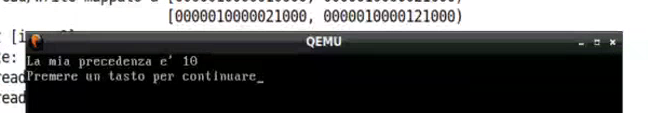
\includegraphics[scale=.95]{img/191.PNG}\end{center}

\chapter{Semafori}
\section{Problemi di mutua esclusione e di sincronizzazione}
Gli utenti del nostro sistema possono creare processi e far eseguire funzioni scelte da loro. Questo utente può definire tanti processi; inoltre, questi processi hanno accesso a una memoria comune (le sezioni \emph{text}, \emph{data} e \emph{bss}).
\paragraph{Altri problemi} Questi processi possono mescolarsi fra loro e possono agire su strutture dati condivise. Come può l'utente garantire che tutto funzioni correttamente? Il problema è simile a quello del modulo sistema (ricordare l'esempio delle liste inconsistenti): li abbiamo risolto con l'atomicità (interruzioni esterne disabilitate, evitiamo eccezioni e chiamate ricorsive di primitive del sistema). Il fatto è che non possiamo permettere all'utente di disattivare le interruzioni, potrebbe non attivarle più e impedirci di riprendere il controllo. Classifichiamo le questioni.
\begin{itemize}
	\item \textbf{Problemi di mutua esclusione}.
	
	L'utente deve fare una o più azioni su una stessa struttura dati, ma non vuole che queste azioni vengano fatte contemporaneamente (cioè non vuole che si mescolino con altre azioni). Si definiscono più processi che possono lavorare sulla stessa lista: queste devono essere mutuamente esclusive, se una cosa è in esecuzione allora l'altra non deve essere in esecuzione.
	
	\item \textbf{Problemi di sincronizzazione}.
	
	 L'utente vuole che una certa azioni si verifichi sempre prima di un'altra. In presenza di un sistema multiprocesso può essere molto complicato (se non impossibile) capire a priori l'ordine in cui i processi saranno eseguiti. Esempio: definizione della struttura dati e lettura della struttura dati, la seconda operazione non ha senso finchè la prima operazione non viene conclusa (\emph{produttore} vs \emph{consumatore}).
\end{itemize}
Non ci addentriamo molto in queste questioni, vedremo solo ciò che ci serve. Attenzione a non confondere le due cose:
\begin{itemize}
	\item nel problema di mutua esclusione non ci interessa l'ordine delle operazioni, ci basta solo non avere il mescolamento delle stesse;
	\item nel problema di sincronizzazione la questione è proprio l'ordinamento.
\end{itemize}

\section{Soluzione ai problemi introdotti: le primitive semaforiche} 
Il sistemista non può risolvere a priori le questioni introdotte, visto che solo l'utente sa cosa vuole fare. Quello che faremo è fornire all'utente le cosiddette \textbf{primitive semaforiche}.
\paragraph{Metafora}  Diamo all'utente la possibilità di definire delle scatole di gettoni, cioè scatole che possono contenere dei gettoni. Posso fare solo due operazioni: inserire un gettone, prendere un gettone. La particolarità sta nella seconda operazione: la scatole è opaca, non sappiamo quanti gettoni ci sono dentro, se nel provare a prendere il getto non trovo nulla allora l'utente si congela e non fa altro, in attesa che qualcun altro aggiunga un gettone.

%\paragraph{Primitive che ci servono} 
%\begin{itemize}
%	\item Primitive per la creazione della scatole di gettoni, indicando il numero di gettoni iniziali (anche zero).
%	\item Primitiva per l'aggiunta di un gettone nella scatola.
%	\item Primitiva per prendere un gettone dalla scatola
%\end{itemize}
%Di per sè non risolvono il problema: l'utente deve imporsi delle regole.


\subsection{Risoluzione del problema della mutua esclusione}
Prendiamo una situazione reale per capire meglio.
\begin{itemize}
	\item Durante l'esame in presenza una sola persona alla volta va in bagno. L'ordine degli studenti non mi interessa, voglio solo evitare che due studenti vadano in bagno insieme. 
	\item Risolviamo la cosa con una scatola avente un solo gettone: chi deve andare in bagno prende il gettone, e lo rimette dopo essere tornato. 
	
	\item \textbf{Problemi di persone che prendono in contemporanea il gettone?} 
	
	No, risolto a priori grazie all'atomicità delle primitive di sistema. 
\end{itemize}
\paragraph{Soluzione cooperativa} La soluzione appena descritta, coi gettoni, è detta \emph{soluzione cooperativa}. Questo perchè ci si aspetta che chi ha preso il gettone lo restituisca. Se ciò non avviene tutti gli altri non possono muoversi.




\subsection{Risoluzione del problema della sincronizzazione}
\paragraph{Cosa vogliamo fare} Supponiamo di avere un'azione $A$ e un'azione $B$. L'ordine nel complesso non ci interessa, ci basta che $A$ venga eseguita prima di $B$, SEMPRE!
\paragraph{Esempio con un buffer}
Prendiamo come esempio un buffer: abbiamo un produttore $P1$, che inserisce un contenuto, e $P2$, consumatore, che lo deve utilizzare.  Se $P2$ arriva prima si troverà ad elaborare dati casuali, e noi non vogliamo che ciò avvenga.\begin{center}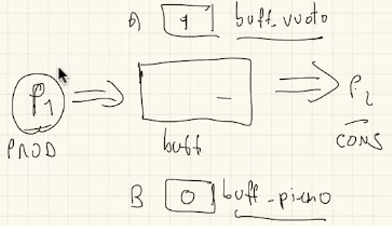
\includegraphics[scale=.8]{img/192.PNG}\end{center}
\begin{itemize}
	\item Stavolta non ho una sola scatola, ma due! 
	\item \textbf{Cosa c'è inizialmente in queste scatole?}  
	
	Una ha un gettone e una è vuota.
	
	\item\textbf{Come si usano queste scatole?}
	
	Possiamo immaginare le due scatole come delle variabili logiche, che hanno come valore $0$ o $1$. Chiamiamo la scatola $A$ \emph{buff$\_$vuoto} e la $B$ \emph{buff$\_$pieno}.
	\begin{itemize}
		\item La scatola $A$ indica se il buffer è vuoto, cioè se $P2$ ha già letto o meno il contenuto presente.
		\item La scatola $B$ indica se il buffer è pieno, cioè se $P2$ ha del contenuto nuovo da leggere.
	\end{itemize}
	Il produttore $P1$ può procedere solo se il buffer è vuoto, quindi con $A=1$ e $B=0$: segue che all'inizio $A$ avrà un gettone e $B$ non avrà gettoni. Il consumatore attende che il buffer si riempa, e agisce solo con $A=0$ e $B=1$. L'idea base è che $P1$ e $P2$, quando svolgono $A$ e $B$ (rispettivamente) levano il gettone dove è presente e lo spostano dove non c'è niente. Quindi
	\begin{itemize}
		\item Il consumatore fa le seguenti cose
		{\small \begin{verbatim}
			PRENDERE(buff_pieno) ---> WAIT(buff_pieno)
			CONSUMARE
			AGGIUNGERE(buff_vuoto) ---> SIGNAL(buff_vuoto)
		\end{verbatim}}
	\item Il produttore fa le seguenti cose
{\small \begin{verbatim}
PRENDERE(buff_vuoto) ---> WAIT(buff_vuoto)
PRODURRE
AGGIUNGERE(buff_pieno) ---> SIGNAL(buff_pieno)
\end{verbatim}}
	\end{itemize}
\item Si osservi che risolvendo questo problema abbiamo affrontato pure la mutua esclusione. In generale i due problemi vanno affrontati singolarmente.
\end{itemize}

\chapter{Implementazione dei semafori nel modulo sistema}

\section{Descrittore di semaforo \emph{des$\_$sem}}
Il \textbf{descrittore di semaforo} è una struttura contenente le informazioni di un semaforo: un contatore (per ricordarci i gettoni presenti) e un puntatore alla lista dei processi in attesa del gettone. 	
\begin{verbatim}
	struct des_sem {
		    int counter;
		    des_proc *pointer;	
	};
\end{verbatim}
Le strutture dati sono poste nel modulo sistema, dunque sono inaccessibili all'utente se non invocando le primitive:
\begin{itemize}
	\item l'accesso è controllato (l'utente non può fare cose che non ci aspettiamo);
	\item si ha atomicità (non si pone la questione della mutua esclusione).
\end{itemize} 
\section{Array dei semafori \emph{array$\_$dess}} 
I semafori non vengono mai deallocati, quindi possiamo allocarli sequenzialmente in un'array.
\begin{verbatim}
	des_sem array_dess[MAX_SEM*2];
\end{verbatim}
\paragraph{Numero massimo di semafori} Creare un'array significa stabilire un numero massimo di semafori. La costante \emph{MAX$\_$SEM}, posta in \emph{include/costanti.h}
\begin{verbatim}
#define MAX_SEM         1024UL
\end{verbatim}
indica il numero massimo di semafori per la modalità utente e per la modalità sistema. L'array \emph{array$\_$dess} è composto da $\text{MAX$\_$SEM}*2$ elementi:
\begin{itemize}
	\item la prima metà dell'array è riservata ai semafori in modalità utente;
	\item la seconda metà ai semafori in modalità sistema.
\end{itemize}
Chiaramente non possiamo permettere l'accesso alla seconda parte dell'array quando ci troviamo in modalità utente. 
\paragraph{Numero di semafori allocati} Con due variabili teniamo a mente il numero di semafori allocati nella prima e nella seconda parte dell'array:
\begin{verbatim}
natl sem_allocati_utente = 0;
natl sem_allocati_sistema = 0;
\end{verbatim}
Considerata l'allocazione sequenziale quanto memorizzato è sufficiente per trovare il primo semaforo non utilizzato.

%Non esiste una primitiva per distruggere un semaforo, la cosa sarebbe molto complessa.
\section{Primitiva per l'allocazione del semaforo}
\subsection{Funzione di utilità \emph{alloca$\_$sem}}
\small 
\begin{verbatim}
natl alloca_sem() {
	    int liv = liv_chiamante();
	    natl i;
	    if(liv == LIV_UTENTE) {
		        if(sem_allocati_utente >= MAX_SEM)
		            return 0xFFFFFFFF;
		        i = sem_allocati_utente;
		        sem_allocati_utente++;
	    }
	    else {
        if(sem_allocati_sistema >= MAX_SEM)
            return 0xFFFFFFFF;
        i = sem_allocati_sistema + MAX_SEM;
        sem_allocati_sistema++;
	    }
	    return i;
}
\end{verbatim}
\normalsize 
\begin{itemize}	
	\item La funzione di utilità \emph{alloca$\_$sem} viene chiamata dalla primitiva \emph{sem$\_$ini}: essa restituisce l'indice del primo semaforo non utilizzato.
	\item Con la funzione di utilità \emph{liv$\_$chiamante} recuperiamo il livello di privilegio prima del lancio della primitiva. 
	\item Tengo conto del valore di \emph{MAX$\_$SEM}, e verifico se ho raggiunto il numero massimo di semafori possibili relativamente a una modalità. Se ciò avviene restituisco
		\begin{verbatim}
			return 0xFFFFFFFF;
		\end{verbatim}
		altrimenti restituisco l'indice del primo elemento array disponibile, e incremento la relativa variabile contatore. 
		\item Ricordarsi che la prima parte dell'array è dedicata alla modalità utente, mentre la seconda alla modalità sistema.
\end{itemize}
\subsection{Primitiva \emph{sem$\_$ini}}
\small 
\begin{verbatim}
// parte "C++" della primitiva sem_ini
extern "C" void c_sem_ini(int val) {
    natl i = alloca_sem();
    
    if(i != 0xFFFFFFFF)
        array_dess[i].counter = val;
    
    esecuzione->contesto[I_RAX] = i;
}
\end{verbatim}
\normalsize 
%\begin{center}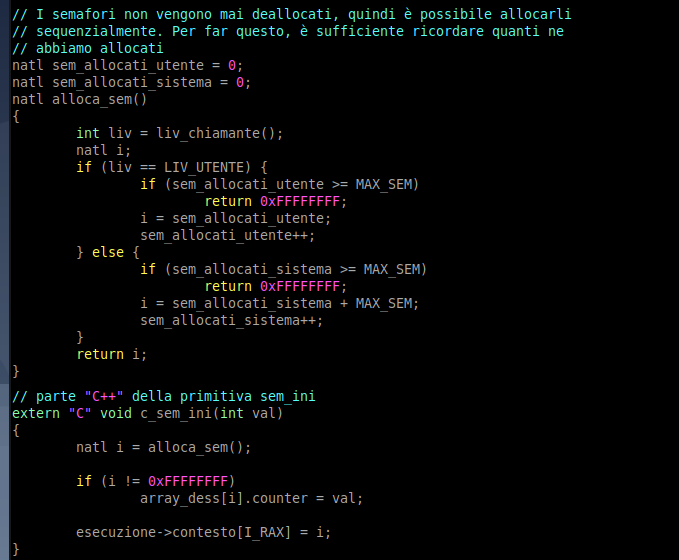
\includegraphics[scale=.8]{img/193.PNG}\end{center}
\begin{itemize}
	\item Per la creazione del semaforo utilizziamo la primitiva \emph{sem$\_$ini}. Il parametro di ingresso  \emph{val} contiene il numero di gettoni iniziali del semaforo.
	\item Con la funzione di utilità \emph{alloca$\_$sem} otteniamo l'indice del primo semaforo non utilizzato dell'array.
	\item Se la funzione non ha restituito il valore di errore manipolo il semaforo avente indice \emph{i}: imposto il \emph{counter} col valore del parametro di ingresso \emph{val} e restituisco \emph{i} aggiornando il contesto di \emph{esecuzione}.
	\begin{verbatim}
		esecuzione->contesto[I_RAX] = i;
	\end{verbatim}
\end{itemize}

\section{Primitive per la gestione dei semafori}

\subsection{Funzione di utilità \emph{sem$\_$valido}} 
\small
\begin{verbatim}
bool sem_valido(natl sem) {
    int liv = liv_chiamante();
    return sem < sem_allocati_utente || (liv == LIV_SISTEMA && sem - MAX_SEM < sem_allocati_sistema);
}
\end{verbatim}
\normalsize
%\begin{center}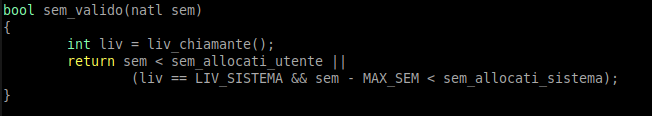
\includegraphics[scale=.9]{img/194.PNG}\end{center} 
\begin{itemize}
	\item Recupero il livello  di privilegio antecedente la chiamata della primitiva con la funzione di utilità \emph{liv$\_$chiamante}.
	\item Uso il valore restituito (posto in \emph{liv}) e il parametro di ingresso \emph{sem} (identificativo di un semaforo) per verificare se questo è valido.
	\begin{itemize}
		\item \textbf{Modalità utente}.
		
		Il semaforo è valido se \emph{sem} è minore del numero di semafori allocati in modalità utente (\emph{sem$\_$allocati$\_$utente}) (ci troviamo nella prima metà dell'array).
		\item \textbf{Modalità sistema}. 
		
		Il semaforo è valido se la differenza tra \emph{sem} e \emph{MAX$\_$SEM} è minore del numero di semafori allocati in modalità sistema (\emph{sem$\_$allocati$\_$sistema}, ci troviamo nella seconda parte dell'array). Dobbiamo anche verificare che il livello del chiamante sia di sistema.  
	\end{itemize}
\end{itemize}

\subsection{Primitiva \emph{sem$\_$wait} (presa del gettone)} 
\small 
\begin{verbatim}
extern "C" void c_sem_wait(natl sem) {
    // una primitiva non deve mai fidarsi dei parametri
    if(!sem_valido(sem)) {
        flog(LOG_WARN, "semaforo errato: %d", sem);
        c_abort_p();
        return;
    }

    des_sem *s = &array_dess[sem];
    s->counter--;
    if(s->counter < 0) {
        inserimento_lista(s->pointer, esecuzione);
        schedulatore();
    }
}
\end{verbatim}
\normalsize 
%\begin{center}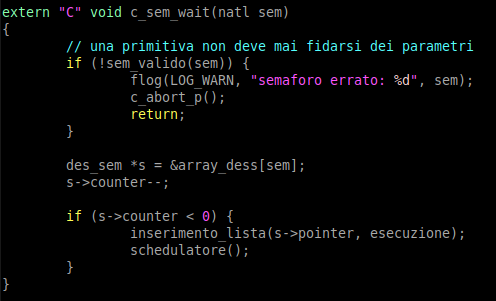
\includegraphics{img/195.PNG}\end{center} 
\begin{itemize}
	\item \underline{Eseguire questa primitiva è un po' come dire \textit{prova a prendere un gettone dal semaforo}}. 
	\item Abbiamo come unico parametro in ingresso l'identificativo del semaforo \emph{sem}.
	\item La prima cosa che facciamo è verificare la validità del semaforo utilizzando la funzione di utilità \emph{sem$\_$valido}. Nel caso in cui l'esito sia negativo si abortisce.
	\item Se l'esito della verifica è positivo si va avanti: si recupera l'indirizzo del relativo semaforo nell'array e si decrementa il contatore \emph{counter} (cioè si leva un "gettone", lo faccio SEMPRE, il valore negativo ha un significato nella primitiva \emph{sem$\_$signal}).
	\item Nel caso in cui il contatore \emph{counter} sia negativo il processo attualmente in esecuzione viene posto nella lista \emph{pointer}, successivamente viene chiamata la funzione \emph{schedulatore}.
	\item La funzione \emph{schedulatore} rimuove la testa di \emph{pronti} e ci porta ad eseguire altri processi. Il processo attuale non potrà essere eseguito finché non ci saranno "gettoni".
\end{itemize}
\subsection{Primitiva \emph{sem$\_$signal} (rilascio del gettone)}
\small 
\begin{verbatim}
extern "C" void c_sem_signal(natl sem) {
    // una primitiva non deve mai fidarsi dei parametri
    if(!sem_valido(sem)) {
        flog(LOG_WARN, "semaforo errato: %d", sem);
        c_abort_p();
        return;
    }

    des_sem *s = &array_dess[sem];
    s->counter++;
    if(s->counter <= 0) {
        des_proc *lavoro = rimozione_lista(s->pointer);
        inspronti(); // preemption
        inserimento_lista(pronti, lavoro);
        schedulatore(); // preemption
    }
}
\end{verbatim}
\normalsize  %\begin{center}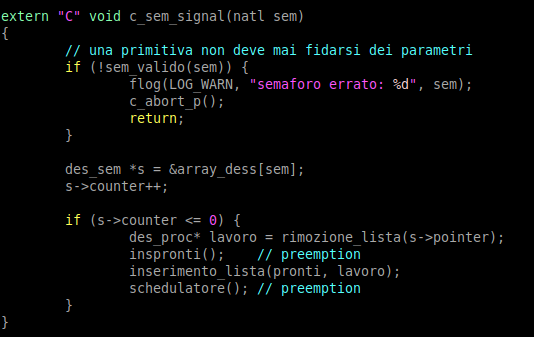
\includegraphics{img/196.PNG}\end{center} 

\begin{itemize}
	\item Abbiamo come unico parametro di ingresso l'identificativo del semaforo \emph{sem}.
	\item La prima cosa che facciamo è verificare la validità del semaforo utilizzando la funzione di utilità \emph{sem$\_$valido}. Nel caso in cui l'esito sia negativo abortisco.
	\item Se l'esito è positivo si va avanti: si recupera l'indirizzo del relativo semaforo nell'array e si  incrementa il contatore (cioè metto un "gettone", lo faccio SEMPRE).
	\item Se il contatore del semaforo è al più uguale a zero allora sono presenti processi che hanno cercato di prendere invano un gettone (e quindi sono in attesa). Quello che facciamo è estrarre uno di questi processi. \item Si ha un meccanismo di \emph{prelazione}.
	\begin{itemize}
		\item Rimuoviamo il processo dalla lista del semaforo, ci ricordiamo dove sta con una variabile temporanea.
		\item Inserisco in testa alla lista \textit{pronti} il processo attualmente in esecuzione con la funzione  \emph{inspronti} (se abbiamo lavorato bene il processo attualmente in esecuzione è quello con la priorità maggiore).
		\item Inserisco nella lista \textit{pronti} anche il processo appena estratto dalla lista del semaforo. 
		\item Chiamo  \textit{schedulatore}, l'esito sarà la scelta di uno dei due processi appena posti in \textit{pronti}.
	\end{itemize}
	\textbf{Perchè abbiamo messo il processo in esecuzione in pronti?} 
	
	Chiediamoci: cosa succede se ho processi con la stessa priorità? Ricordiamo il codice di \emph{inserimento$\_$lista}: a parità di priorità diamo un'ordinamento FIFO (chi prima arriva esce per primo). Il fatto è che inserire il processo attualmente in esecuzione in lista \emph{pronti} con \emph{inserimento$\_$lista} (e non con \emph{inspronti}) significherebbe porlo in lista dopo altri processi aventi la stessa priorità, se presenti. Con il codice scritto ci assicuriamo che il processo attualmente in esecuzione non venga sospeso se sono presenti altri processi aventi la stessa priorità: è una sottigliezza, non è sbagliato fare diversamente.
\end{itemize} 

\begin{framed}
\noindent \textbf{Stati bloccati}.

\noindent I semafori permettono l'implementazione dei cosiddetti \emph{stati bloccati}: ogni semaforo rappresenta un possibile stato bloccato, dove l'attesa dipende dal diverso significato che attribuiamo a un certo semaforo.
\end{framed} 

\begin{framed}
	\noindent \textbf{Promemoria sull'atomicità delle primitive}.
	
	\noindent Le primitive semaforiche non possono essere usate all'interno di un'altra primitiva, ne romperebbero l'atomicità. La questione sarà affrontata nel capitolo sulle periferiche, dove introdurremo delle novità.
\end{framed} 

\chapter{Premesse sulla paginazione}
La paginazione è l'argomento che storicamente confonde di più gli studenti. Si tenga conto che l'argomento sarà affrontato anche nel corso di \textit{Sistemi Operativi}.
\section{Recap con prime questioni}
\begin{itemize}
	\item \textbf{Memory mapped I/O}. 
	
	Lo spazio di indirizzamento include la RAM (che occupa una minima parte dello spazio), ma anche periferiche come APIC, memoria video in modalità testo, memoria video in modalità grafica. La cosa ci ha creato problemi relativamente alle periferiche \emph{memory mapped}: la cache deve essere disattivata, non può memorizzare cacheline relativamente ad istruzioni di I/O. L'unica cosa che possiamo fare è distinguere le operazioni a partire dagli indirizzi.
	\item \textbf{Protezione}. 
	
	Abbiamo diviso la memoria RAM in due parti: la parte $M1$ per il sistema e la parte $M2$ per l'utente. I meccanismi di protezione fanno sì che l'utente non possa accedere in alcun modo alla prima area di memoria (nè operazioni di lettura, nè di scrittura).  Abbiamo dei problemi relativi all'\textbf{isolamento tra processi}. La protezione agisce anche sulle istruzioni di un programma: posso leggerle ma non modificarle. Inoltre, viene vietato l'utilizzo dell'indirizzo $0$, poiché \emph{nullptr} (anche in modalità sistema).
	\item \textbf{Multiprogrammazione}. 
	
	Abbiamo anche detto che ogni volta che attraversiamo il gate ed effettuiamo un cambio di processo dobbiamo memorizzare il \emph{contesto}. Il contesto non si limita ai soli registri, ma anche al contenuto della memoria. Se vogliamo fare i precisi diventa necessario spostare l'intera area di memoria nell'hard disk (cioè in qualcosa di più grande). Questa cosa funziona molto bene con memorie RAM piccole, ma adesso è problematica (oggi fare uno spostamento del genere significa lavorare con diversi GB).
\end{itemize} 
\clearpage 
\section{Idea di base: tenere insieme informazioni di più processi} Abbiamo bisogno di un meccanismo che minimizzi gli spostamenti tra RAM e hard disk, limitandoci al minimo indispensabile. L'idea è tenere in memoria RAM le informazioni relative a più processi, cioè trattare la RAM come una sorta di cache dell'hard disk. Si considerino le seguenti problematiche.
\begin{itemize}
	\item \textbf{Dimensione massima di ogni processo} 
	
	La prima cosa che dobbiamo chiederci è di quanto spazio ha bisogno ogni processo. Dobbiamo tenere conto delle seguenti aree:
	\begin{itemize}
		\item \emph{text} (codice programma) e \emph{data} (variabili globali), dimensione nota al collegatore e costante per tutta l'esecuzione del programma;
		\item pila e \emph{heap}, aree di memoria (inizialmente vuote) che possono espandersi durante l'esecuzione del programma.
	\end{itemize}
	L'area di memoria di un processo è organizzata così
	\begin{center}
		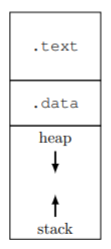
\includegraphics{img/208.PNG}
	\end{center}
	\emph{heap} e pila stanno in un'area unica, con direzioni di espansione opposte.  
	
	\noindent \textbf{Soluzione}. Quello che faremo è porre dimensione massima per l'area dedicata a \emph{heap} e pila. Solitamente si pone un valore di default. 
	
	\item \textbf{Isolamento tra i processi}	
	
	Abbiamo detto che l'idea base è mettere insieme, nella RAM, più processi. Senza il ricorso al meccanismo della protezione il processo in esecuzione potrebbe intervenire sullo stato dei processi non in esecuzione.
	
	\noindent \textbf{Soluzione}. L'idea risolutiva potrebbe essere l'aggiunta di due nuovi registri nella CPU: LINF (limite inferiore) ed LSUP (limite superiore). Segue l'inserimento di questi due registri nel \emph{contesto} in \emph{des$\_$proc}. \begin{itemize} 
		\item Chiaramente i due registri sono scrivibili solo a livello sistema.
		\item Se ci troviamo a livello utente la CPU controlla che ogni accesso memoria sia compreso tra LINF ed LSUP, altrimenti lancia un'eccezione.
		\item Ogni volta che un processo viene caricato dall'hard disk il sistema deve inizializzare gli appositi campi \emph{contesto} con l'indirizzo finale e iniziale della parte di memoria occupata dal processo.
		\item Ogni volta che si cambia processo si aggiorna il contenuto di LINF ed LSUP nel processore, prendendo come valori quelli relativi al processo entrante.
	\end{itemize}  
	Attenzione: questa soluzione non è quella definitiva (quando introdurremo la paginazione vedremo perchè non servono questi registri).
	
	\item \textbf{Caricamento a indirizzi variabili}
	
	L'indirizzo dove andiamo a caricare il processo non è più chiaro come prima: il processo può essere caricato ovunque e la sua posizione dipende anche dagli altri processi posti nella RAM. L'indirizzo dove carichiamo il processo non è quindi noto durante compilazione e collegamento.
	\begin{itemize}
		\item \textbf{Grosso problema}. Se io rimuovo un processo e lo metto in un punto diverso della memoria gli indirizzi relativi al processo non sono più validi, dovrei correggerli rispetto alla nuova posizione: questa cosa non è possibile, poichè gli indirizzi sono indistinguibili.
		\item \textbf{Soluzione}. La soluzione è utilizzare il registro LINF come indirizzo di base. L'indirizzo $x$ in un processo è diverso dall'indirizzo $x$ in un altro processo: nel programma ci limitiamo a indicare l'offset, che si somma a LINF per ottenere l'indirizzo vero e proprio a cui puntare. 
	\end{itemize}
	Attenzione: questa soluzione non è quella definitiva (quando introdurremo la paginazione vedremo perchè non serve il registro LINF e come facciamo a ricondurci al cosiddetto \emph{indirizzo fisico}).
\end{itemize}
\section{Step successivo: memoria virtuale e indirizzi virtuali}
Riflettiamo un po' di più sull'ultima questione affrontata: quella degli indirizzi variabili. Fino ad oggi abbiamo utilizzato solo ed esclusivamente i cosiddetti \textbf{indirizzi fisici}. Adesso introduciamo gli \textbf{indirizzi virtuali} e la \emph{memoria virtuale}.
\begin{itemize}
	\item \underline{Il codice del programma relativo a un processo utilizza esclusivamente \emph{indirizzi virtuali}}.
	\item Questi \emph{indirizzi virtuali} sono relativi al processo, cioè l'indirizzo $x$ di un presunto processo $P1$ non sarà uguale all'indirizzo $x$ di un processo $P2$.
	\item Se consideriamo la soluzione provvisoria per gli indirizzi otteniamo quello fisico così
	\[\text{Indirizzo fisico}=\text{LINF}+\text{Indirizzo virtuale}\]
\end{itemize}

\paragraph{Cioè?} Dobbiamo distinguere lo \emph{spazio di indirizzamento fisico} (dove troviamo RAM e qualunque periferica) dallo \emph{spazio di indirizzamento virtuale}. I processi non hanno alcun accesso allo spazio di indirizzamento fisico: vedono solo lo spazio di indirizzamento virtuale, che è una sorta di mondo immaginario dove troviamo la \emph{memoria virtuale}. In questa memoria sono presenti le solite parti: \emph{text}, \emph{data}, \emph{heap} e \emph{stack}.
\begin{center}
	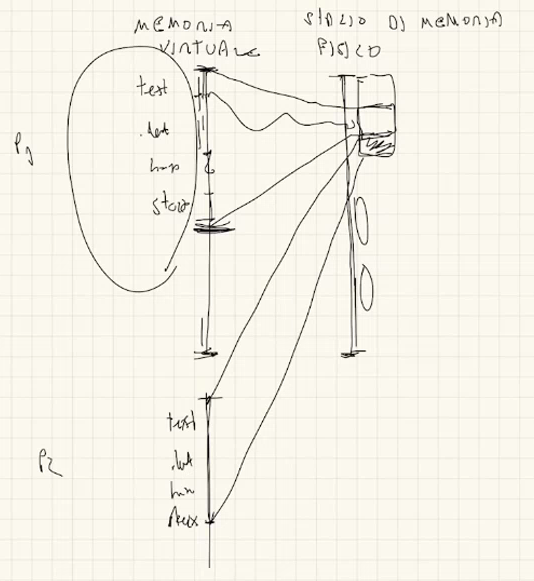
\includegraphics[scale=.65]{img/209.PNG}
\end{center} 
L'hardware, attraverso una unità che vedremo più avanti, trasforma gli indirizzi di \emph{text}, \emph{data}, \emph{heap} e \emph{stack} in indirizzi dello spazio di memoria fisico (\textit{un po' come i film Western dove di una casa c'è solo la facciata}, cit.).
\subsection{Scopo del Kernel} Quello che avremo è una situazione dove il programma si interfaccia con una CPU e una RAM virtuali.
\begin{itemize}
	\item La CPU è il contesto che abbiamo salvato nel descrittore di processo, che verrà caricato nella CPU vera (si aggiorna lo stato della CPU fisica in divisione di tempo, ma si rappresenta lo stato della CPU virtuale).
	\item La memoria RAM non viene gestita in divisione di tempo (come ipotizzato all'inizio), ma in divisione di spazio: la RAM contiene, in contemporanea, più immagini di processi diversi.
\end{itemize} 
Tutte queste cose sono affrontate dal \emph{kernel}.

\paragraph{Definizione di \emph{kernel} su Wikipedia} \textit{Un kernel, in informatica costituisce il nucleo o core di un sistema operativo, ovvero il software che fornisce un accesso sicuro e controllato dell'hardware ai processi in esecuzione sul computer. Dato che possono eventualmente esserne eseguiti simultaneamente più di uno, il kernel può avere anche la responsabilità di assegnare una porzione di tempo-macchina (scheduling) e di accesso all'hardware a ciascun programma (multitasking)}.

\clearpage 

\section{Tutto finito?}

Il meccanismo di cui abbiamo parlato fino ad ora presenta due svantaggi:
\begin{enumerate}
	\item Come possiamo condividere parte della memoria tra due o più processi?
	\item Cosa succede se dobbiamo caricare un processo, ma lo spazio in memoria è frammentato in porzioni troppo piccole? Questo problema potrebbe essere risolto
	\begin{enumerate}
		\item ricompattando lo spazio (ma questo significherebbe copiare un'intera porzione di memoria da una zona a un'altra), oppure
		\item spezzare la memoria di un processo in più porzioni e gestire ciascuna di queste separatamente.
	\end{enumerate}
\end{enumerate}
La soluzione (b) è la più interessante, visto che permette di risolvere anche il primo problema. 
\begin{center}
	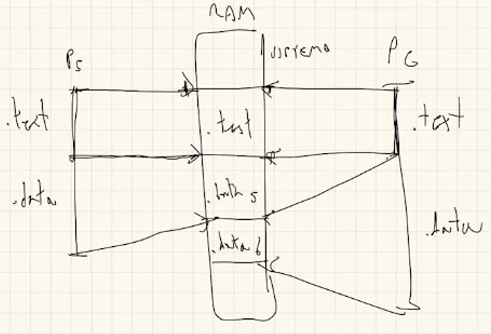
\includegraphics[scale=.8]{img/211.PNG}
\end{center} Tutto questo ci porta a parlare della \textbf{paginazione}, dove parti diverse dello spazio di indirizzamento di un processo si traducono in modo diverso (il passaggio da indirizzi virtuali a indirizzi fisici).

\chapter{Paginazione}
Tradurre gli indirizzi virtuali in indirizzi fisici singolarmente è una cosa veramente improponibile. 
\paragraph{Cosa facciamo?}
\begin{itemize}
	\item Dividiamo lo spazio di indirizzamento virtuale in regioni naturali dette \emph{pagine}.
	\item Dividiamo lo spazio di indirizzamento fisico in regioni naturali dette \emph{frame}.
\end{itemize}
Pagine e frame hanno la stessa dimensione: $4\,\text{KiB}$ (0x1000 in esadecimale). La pagina viene inserita in un frame e si identifica perfettamente con esso: non esiste una pagina posta tra frame diversi.
\paragraph{Traduzione degli indirizzi in una pagina} Tutti gli indirizzi posti in una pagina sono tradotti in maniera contigua (la traduzione effettiva avviene nei bit più significativi, non nell'offset).
%\begin{center}
%	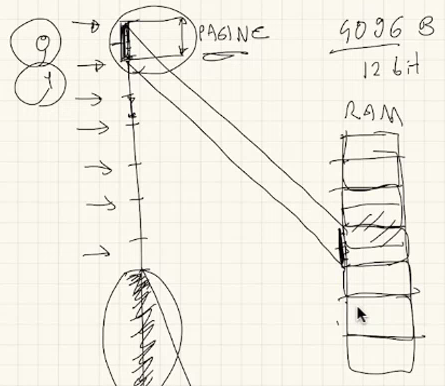
\includegraphics[scale=.8]{img/212.PNG}
%\end{center}
\section{\emph{Memory Management Unit} (MMU)}
Abbiamo introdotto l'organizzazione in pagine, ma non abbiamo ancora detto come gestiremo il passaggio da indirizzo virtuale a indirizzo fisico, tenendo conto che la traduzione dovrà essere diversa per ogni pagina. Introduciamo l'\textbf{unità di gestione della memoria} tra CPU e Cache.
\begin{itemize}
	\item Si osservi che la MMU non ha un buco come lo spazio di indirizzamento: negli indirizzi presenti si ha un salto dall'ultimo indirizzo prima del buco al primo indirizzo dopo il buco.
	\item La cache fa parte del mondo fisico, può ignorare l'introduzione della \emph{Memory Management Unit} (MMU). La MMU traduce gli indirizzi virtuali in base alla traduzione attiva in un certo istante: la struttura dati utilizzata dalla MMU può essere immaginata come un insieme di \textit{tabelle di corrispondenza} (una per processo). Queste tabelle sono un esempio di struttura dati condivisa tra hardware e software: quest'ultimo (il kernel) stabilisce quali tabelle ci sono e quali sono attive.
\end{itemize}
\begin{center}
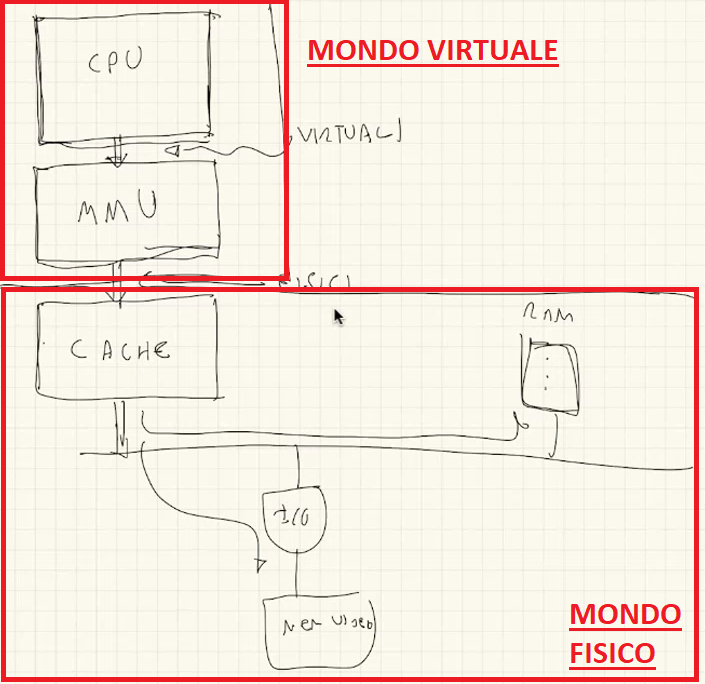
\includegraphics[scale=.5]{img/213.PNG}
\end{center}

\subsection{Passaggio da indirizzo virtuale a indirizzo fisico} 
\begin{center}
	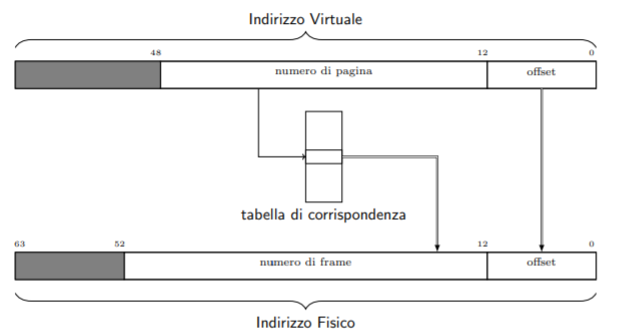
\includegraphics[scale=.9]{img/214.PNG}
\end{center}
\begin{itemize}
	\item Nell'indirizzo indicato dalla CPU si distingue l'\emph{offset} (bit meno significativi) dal \emph{numero di pagina} (bit più significativi).
	\item Il numero di pagina va in ingresso nella tabella di corrispondenza relativa al processo: l'indice posto in ingresso mi restituisce il corrispondente  \emph{numero di frame}. 
	\item Ogni tabella di corrispondenza ha una riga per ogni possibile pagina (non poche, visto il numero di bit riservati al numero di pagina). 
\end{itemize}
\paragraph{Attenzione al numero di bit} Gli indirizzi fisici fanno riferimento allo spazio di indirizzamento fisico, quelli virtuali allo spazio di indirizzamento virtuale. Il numero di bit massimo è $64$, varie generazioni di CPU implementano indirizzi virtuali su un numero inferiore di bit. La questione dipende dal modello della CPU, tutto lì (cit.). 

\subsection{Contenuto delle tabelle di corrispondenza} Ciascuna riga delle tabelle di corrispondenze è grande 8 byte: il numero di frame si trova nella posizione in cui si troverebbe all'interno dell'indirizzo (per comodità del programmatore, in questo caso si va dal bit 12 al bit 52). Le righe non contengono solo il corrispondente \emph{numero di frame}, ma anche una serie di flag (di cui non ci interessa la posizione):
 \begin{itemize}
 	\item un flag $U/S$ che mi indica se la pagina può essere acceduta solo a livello utente o anche a livello sistema (quindi distinguo attraverso questo flag i frame relativi all'area riservata al livello sistema dai rimanenti\footnote{Viene meno la necessità di un registro che indica l'indirizzo limite tra area riservata al sistema e il resto.});
 	\item un flag $R/W$ che mi indica se la scrittura nella pagina è permessa o no;
 	\item un flag $P$ (presenza) che mi dice se la traduzione è valida (quindi se l'indirizzo corrisponde, al di la del livello di privilegio). Si utilizza per marcare le pagine che il processo non usa (che avranno $P=0$);
 	\begin{itemize}
 		\item Il flag $P$ può essere utilizzato per vietare l'utilizzo dell'indirizzo $0$ (mi basta porre $0$ nella pagina relativa). Nel caso di accesso a una pagina con $P=0$ il processore solleva un'eccezione \emph{page fault} (fault perchè il sistema potrebbe aggiustare lo stato della memoria e rieseguire l'istruzione attraverso la \emph{paginazione su domanda}, che vedremo a Sistemi Operativi\footnote{Uno dei pochi esempi di \emph{fault} effettivamente risolti}).
 	\end{itemize}
 	\item i flag PWT (\emph{Page Write Through}) e PCD (\emph{Page Cache Disable}), con cui la MMU trasmette dei comandi alla cache (il secondo ordina alla cache di non intercettare l'operazione, il primo chiede di utilizzare alla cache di usare la politica \emph{write-through}).
 	\begin{itemize}
 		\item Il flag PCD è utile per tutte le pagine che contengono indirizzi di registri di I/O mappati in memoria, invece che locazioni di memoria (per esempio l'APIC). 
 		\item Il flag PWT è utile per quanto riguarda la parte di indirizzi relativa alla memoria video: vogliamo che la scrittura vera arrivi nella memoria video, e che non rimanga in cache.
 	\end{itemize}
 \end{itemize}


\paragraph{Flag per la paginazione su domanda} Abbiamo i bit $A$ e $D$ che sono legati all'implementazione della paginazione su domanda. La MMU setta il bit $A$ di una entrata quando la MMU accede alla relativa entrata per fare una traduzione, mentre setta il bit $D$ se l'accesso all'indirizzo relativo alla pagina era in scrittura.
\paragraph{Bit NX} Ulteriore bit è il \emph{Not executable}. Se durante l'operazione di fetch di un'istruzione abbiamo $NX=1$ per la relativa pagina allora il processore genera un'eccezione.





%I processi non ci dicono l'indirizzo di memoria RAM a cui vogliono accedere, ma solo l'offset. A runtime il registro LINF non viene usato come limite, ma per essere sommato all'offset.
%- Lo spazio di indirizzamento del processore presenta, oltre alla RAM, periferiche: APIC, memoria video in modalità grafica, memoria video in modalità testo (che nasconde parte della RAM), abbiamo parlato di \emph{Memory Mapped I/O}. La cosa è problematica per la \emph{Cache}, che normalmente lavora solo con lo spazio di memoria. Vogliamo disattivarla, l'unica cosa che può distinguere due operazioni è l'indirizzo. La soluzione è limitare l'accesso alle periferiche sulla base degli indirizzi, e non dell'istruzione eseguita.

%Protezione:
%Negli accessi in memoria la cosa è più sofisticata rispetto a dire livello utente o livello sistema (cosa che comunque è presente).
%- Nella parte dedicata all'utente c'è un qualcosa di più: pensiamo ai programmi, che possono essere letti ma non sovrascritti.
%- Il \textit{null pointer} è rappresentato con l'indirizzo 0, quindi quell'indirizzo non può essere utilizzato. Addirittura è possibile stabilire l'inaccessibilità dell'indirizzo pure in modalità sistema. 

\section{MMU e modulo sistema} 
Facciamoci una domanda: siamo obbligati a mappare gli indirizzi relativi al modulo sistema nello spazio di indirizzamento virtuale dei vari processi? Sì: se siamo a livello utente e sollevo un'eccezione la CPU inizia a fare un po' di cose, come consultare l'IDT e il TSS, o scrivere dentro la pila sistema. Tutti questi indirizzi saranno tradotti dalla MMU, dunque in assenza di mapping la gestione delle interruzioni non è possibile

\paragraph{Cosa faremo} La cosa più semplice è mappare tutta la memoria di sistema: quando siamo a livello utente e avviene un passaggio a livello sistema la CPU troverà tutto ciò che le serve (visto che tutto è mappato). In questa parte di indirizzamento mapperemo tutta la zona di RAM che contiene il codice e le strutture dati presenti nel modulo sistema. Cosa importante
\[\boxed{\text{Tutto è mappato agli stessi indirizzi in ogni processo}}\]
\paragraph{Tabelle di corrispondenza e cambio di processo} Se il sistema vuole fare un cambio di processo allora deve cambiare la tabella di corrispondenza. Se non facciamo ciò l'\textit{Instruction pointer} va avanti interpretando gli indirizzi in modo inaspettate (traduco col contenuto della tabella di corrispondenza del vecchio processo, non con quella del processo in esecuzione).

\paragraph{Aspetto complicato} Scrivere codice sistema essendo costantemente consapevoli della differenza tra indirizzi fisici e indirizzi virtuali. Lavorando a livello utente questo ignora che i suoi indirizzi sono virtuali: gli utenti usano solo questi e non hanno interesse sugli indirizzi fisici.

\section{Esempio: indirizzi virtuali e fisici in un programma in esecuzione} 
Scriviamo un programma dove dichiariamo una variabile e ne stampiamo l'indirizzo
\begin{verbatim}
	#include <iostream>
	
	int var;
	int main() {
		     std::cout << "&var: "<< &var << "\n";
	}
\end{verbatim}
Compiliamo
\begin{verbatim}
	g++ -o myprog.cc -no-pie myprog.cc
	./myprog
\end{verbatim} 
Otteniamo
\begin{verbatim}
	&var: 0x404174
\end{verbatim}
L'indirizzo stampato è l'indirizzo scelto dal collegatore: compilatore, collegatore e programmatore sono consapevoli solo dell'esistenza di questo indirizzo virtuale (per noi è l'unico indirizzo vero).
\paragraph{Chiediamo l'indirizzo fisico} Se abbiamo livelli di privilegio sufficienti possiamo chiedere l'indirizzo fisico invece di quello virtuale. Modifichiamo il programma per mantenerlo in vita
\begin{verbatim}
#include <iostream>
	
int var;
int main() {
     std::cout << "&var: "<< &var << "\n";
		
     for(;;) {
          sleep(1);
     }
}
\end{verbatim}
dove \emph{sleep} è l'equivalente unix della \emph{delay}, col numerino che esprime i secondi. Eseguiamo il programma e mentre questo cicla chiediamo col terminale il processor identifier
\begin{verbatim}
	pgrep myprog
\end{verbatim}
successivamente eseguiamo la seguente istruzione
\begin{verbatim}
	sudo ./virt_to_phys 1922 0x404174 // verra' richiesta la password
\end{verbatim}
otteniamo l'indirizzo fisico \textbf{0x49512174}, completamente diverso dall'indirizzo virtuale (tranne che nell'offset, le tre cifre esadecimali meno significative costituiscono l'offset all'interno della pagina).
\begin{itemize}
	\item La variabile var si trova nella pagina 404 all'offset 174.
	\item La MMU trasforma il numero di pagina nel numero di frame 495121, non l'offset.
\end{itemize}
Proviamo ad eseguire un'altra istanza del programma, senza chiudere la precedente. Con le stesse cose fatte prima otteniamo l'indirizzo fisico \textbf{0x4ed18174}: non è cambiato l'offset (174), ma è cambiato il numero di frame (4ed18). Ognuno vive nel suo mondo senza conoscere l'esistenza dell'altro.

\section{MMU all'opera}
\small
Nelle diapositive seguenti viene spiegato nel dettaglio il comportamento della MMU con le sue \emph{tabelle di corrispondenza}. 
\begin{itemize}
	\item Viene introdotto un programma in C++ che agisce su uno spazio di indirizzamento virtuale. Si suppone, per ragioni di semplicità, che lo spazio di indirizzamento virtuale sia di $32\,\text{KiB}$ (gli indirizzi vanno da 0000 a 7fff).
	\item Lo spazio di indirizzamento viene diviso in 8 pagine, ciascuna da $4\,\text{KiB}$ (nulla di nuovo).
	\item Le pagine $0$ e $1$ sono riservate al sistema.
	\item La pagina $2$ contiene il codice del programma (da 2000 a 2fff).
	\item Le pagine $3$ e $4$ contengono la variabile \emph{buf}.
	\item La pagina $7$ viene usata come pila.
\end{itemize}
Successivamente viene introdotto un secondo processo, più piccolo. Le diapositive mostrano come la MMU operi con due processi.
\normalsize 

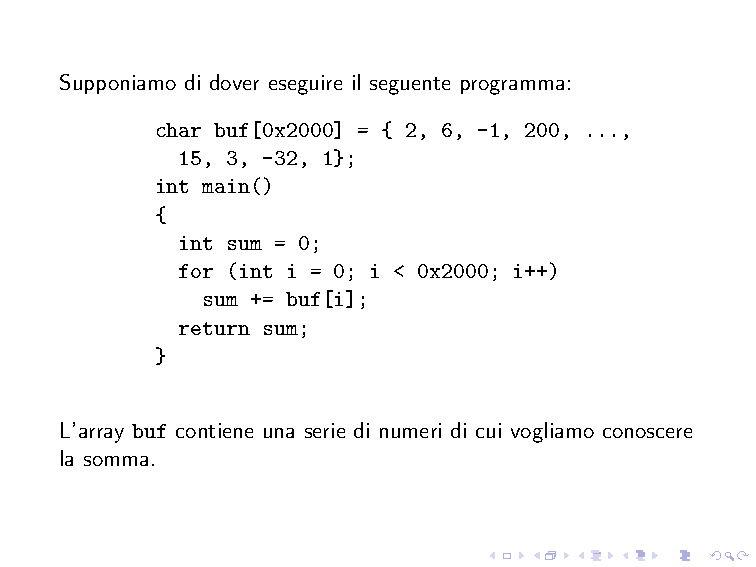
\includepdf[pagecommand={\thispagestyle{plain}},frame,scale=0.93,frame,nup=2x3,pages=-]{pdf/supermmu}

\section{Tabelle di corrispondenza multilivello (\emph{bitwise trie})}
\paragraph{Quanto è grande una tabella di corrispondenza?} Supponiamo di avere uno spazio di $2^{48}$ byte: considerato che ogni pagina è grande $2^{12}$ byte otteniamo il seguente numero di pagine
\[\frac{2^{48}}{2^{12}}=2^{36}\]
La dimensione di ogni entrata è di 8 byte: segue la dimensione della tabella di corrispondenza
\[2^{36} \times 8\,\text{byte}=512\,\text{GiB}\]
Morale della favola: è difficile avere un dispositivo che mi possa contenere una sola di queste tabelle. Ci serve una struttura dati che mi permetta di associare una chiave a un valore
\[\boxed{\text{Chiave (Numero di pagina)} \longrightarrow \text{Valore (Numero di frame)}}\]
\paragraph{Struttura dati} La struttura dati immaginata è una variante del \emph{trie}
: il \emph{bitwise trie}. Con \emph{trie} intendiamo strutture dati ad albero con cui mappiamo chiavi di tipo stringa. Supponiamo di avere le seguenti associazioni
\[\begin{array}{l}\text{trip} \longrightarrow \text{viaggio}\\\text{tree} \longrightarrow \text{albero}\\\text{hill} \longrightarrow \text{collina}\\\text{hot} \longrightarrow \text{caldo}\\\text{house} \longrightarrow \text{casa} \end{array}\]
Otteniamo il seguente albero:
\begin{center}
	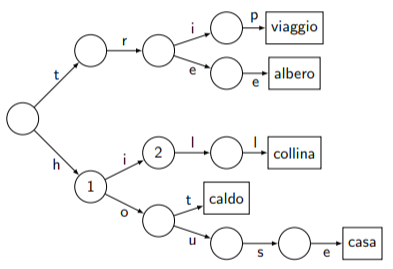
\includegraphics{img/215.PNG}
\end{center}
\begin{itemize}
	\item I caratteri guidano i nostri movimenti all'interno dell'albero: gli archi sono marcati con i caratteri delle chiavi e il valore associato ad ogni chiave si trova nella foglia che si raggiunge partendo dalla radice e seguendo il percorso indicato dalla chiave. 
	\item L'inserimento di una nuova associazione chiave-valore comporta una visita nell'albero come in una ricerca, con la creazione di eventuali nodi mancanti fino alla foglia che deve contenere il valore.
\end{itemize}
Tenendo conto che il trie si basa sulla codifica ASCII possiamo immaginarci un'implementazione dove ogni nodo consiste in un array di 128 entrate: ogni elemento dell'array è nullo o contiene un puntatore ad un altro nodo (quindi ad un altro array).

\paragraph{\emph{bitwise trie}} Il bitwise trie è una variante che prevede al posto dei caratteri gruppi di bit della chiave. L'indirizzo della radice è posto nel registro \emph{CR3} della MMU.
\begin{itemize}
	\item Il numero di pagina è composto da 36 bit, che raggruppiamo in quattro gruppi da 9 bit ciascuno. Nello scorrimento dell'albero consideriamo i gruppi \textbf{da quelli con le cifre più significative a quelli con le meno significative}.
	\item Ogni nodo del bitwise trie risulterà essere una tabella di $2^9=512$ entrate. Ciascuna entrata è un puntatore che può essere nullo, o rimandare a un nodo successivo.
	\item Sappiamo che ogni entrata ha dimensione di 8 byte, dunque otteniamo che ogni tabella ha dimensione
	\[512 \cdot 8\,\text{byte}=4096\,\text{byte}\]
	\item L'albero ha al più 4 livelli, numerati dalla radice in senso decrescente (da $4$ ad $1$)
	\begin{center}
		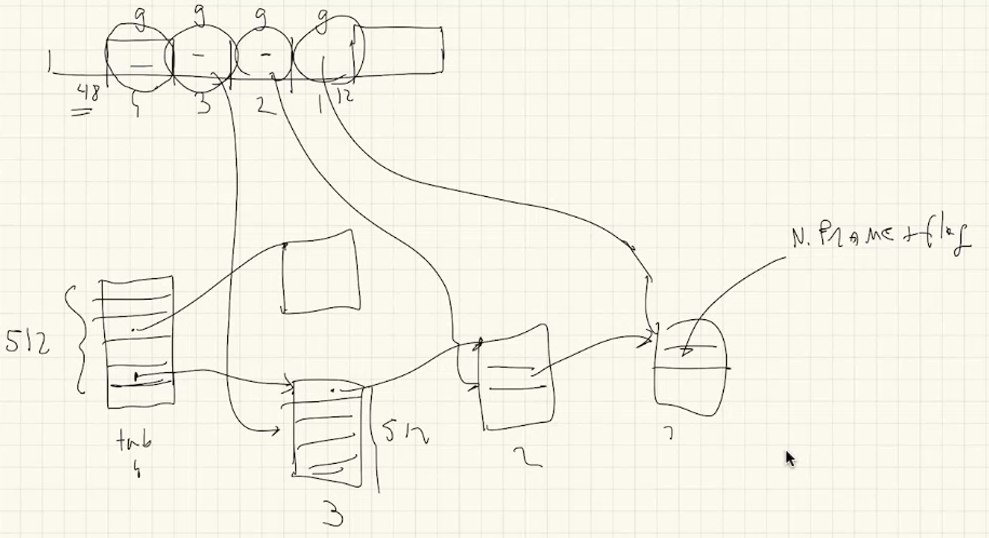
\includegraphics[scale=.55]{img/216.PNG}
	\end{center}
	Se noi mettiamo insieme tutti i nodi, tutte le tabelle, otteniamo la tabella iniziale, ma a dimensione maggiore. Cio è valido solo se realizziamo tutti i sotto-alberi possibili (non abbiamo alberi dove il processo non ha mappato niente). 
	\item Le foglie hanno la stessa struttura dei nodi, l'unica differenza sta nel significato delle entrate (che contengono non un puntatore, ma il numero di frame). 
	\item Ogni riga delle tabelle ha la stessa struttura. Differenza rispetto alle tabelle viste all'inizio introducendo la MMU è la presenza di un maggior numero di bit: questo a causa dell'allineamento naturale delle tabelle (4096 byte), che impone i primi 12 bit meno significativi dell'indirizzo di una tabella uguali a zero. Alcuni bit non sono presenti (per esempio D), mentre altri sono presenti ma hanno un significato radicalmente diverso.
	\item il \emph{page fault} viene generato non appena si individua una riga con $P=0$.
	\item \textbf{Regola per le scritture}. La scrittura è permessa solo se è permessa da tutti i livelli.
	\item \textbf{Regola per l'accesso da livello utente}. L'accesso a livello utente è consentito solo se consentito da tutti i livelli.
\end{itemize}
\begin{framed}
\noindent \textbf{Recap}
\begin{itemize}
	\item Abbiamo definito un architettura con la MMU posta tra CPU e Cache, distinguendo un "mondo fisico" con indirizzi fisici da un "mondo virtuale" con indirizzi virtuali (CPU e la MMU, dunque il software).
	\item La MMU, in ogni istante, avrà una traduzione attiva: un albero trie con cui associo un indirizzo fisico a un indirizzo virtuale (ottengo l'indirizzo fisico sostituendo, nell'indirizzo virtuale, il numero di pagina col numero di frame). La CPU contiene un registro, detto CR3, col numero di frame dove si trova la radice dell'albero attivo (l'albero si trova nella RAM, attenzione).
	\item Percorro l'albero utilizzando le varie parti che caratterizzano il numero di pagina: nella foglia troverà il numero di frame. Ricordiamoci che oltre al numero di frame abbiamo altre informazioni associate al numero di pagina.
	\item La struttura ci permette di evitare di associare un frame a qualunque pagina: dove non si può andare l'albero non prosegue, con $P=0$.
\end{itemize}   
\end{framed}
\paragraph{Domanda sugli indirizzi della struttura dati} Questa è una struttura dati preparata dal sistema e utilizzata dall'hardware (MMU). Nelle varie tabelle sono presenti puntatori ad altre tabelle nella RAM. Ci siamo chiesti: questi puntatori sono indirizzi virtuali o fisici? 
\begin{itemize}
	\item Fisici, altrimenti si genererebbe una sorta di loop (come faccio a muovermi tra le varie tabelle-nodo se ogni puntatore deve essere a sua volta tradotto attraverso le tabelle stesse?). \textbf{Emerge il problema di gestire questi passaggi}.
\end{itemize}

\paragraph{Come fa il software ad accedere a qualunque cosa?} Per accedere a una qualunque entità abbiamo bisogno delle seguenti cose:
\begin{enumerate}
	\item un indirizzo fisico per l'entità;
	\item un indirizzo virtuale associato all'indirizzo fisico dell'entità;
	\item la conoscenza da parte del software dell'indirizzo virtuale (all'utente non serve conoscere l'indirizzo fisico, il software lavora solo con indirizzi virtuali)
\end{enumerate} 

\subsection{Utente e indirizzi virtuali e fisici}
 Per l'utente la vita è facile: conosce solo l'indirizzo virtuale. In un programma utente si dichiara una variabile globale, e il collegato sceglie un indirizzo virtuale per questa variabile. La variabile acquisisce un indirizzo fisico perchè il sistema caricherà la sezione data in una pagina, quindi in qualche frame. Il sistema, interpretando il file ELF, vedrà che il collegatore voleva he quella variabile si trovasse a un certo indirizzo virtuale: si crea così una corrispondenza tra indirizzo fisico e indirizzo virtuale.
 
 
 \paragraph{stack} Per quanto riguarda lo stack non ci sono problemi: creiamo la corrispondenza tra indirizzo fisico e indirizzo virtuale, a quel punto rendo conoscibile  l'indirizzo virtuale mettendolo  nel registro RSP.
 
 
 
 \subsection{Sistemi e indirizzi virtuali e fisici}
 Per il sistema le cose sono più difficili: deve essere consapevole in modo costante della differenza tra indirizzi fisici e indirizzi virtuali. In alcune situazioni gli indirizzi fisici sono irrinunciabili: le comunicazioni col bus mastering, l'aggiornamento delle tabelle di corrispondenza. Per memorizzare l'albero ci servono dei frame
 	\begin{center}
 	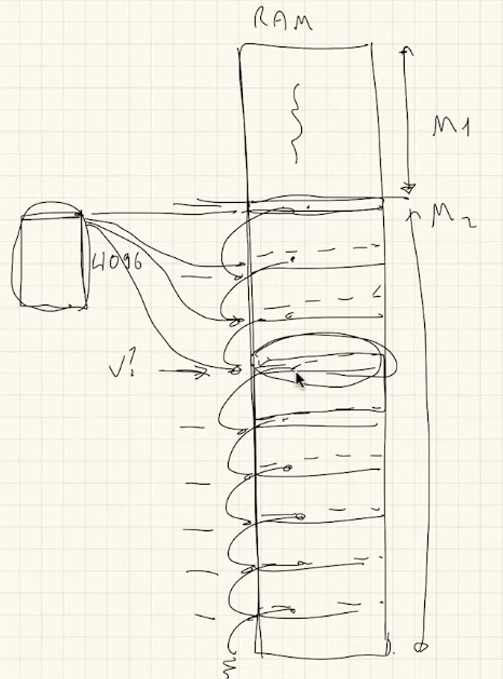
\includegraphics[scale=.7]{img/217.PNG}
 \end{center}
 in ciascun frame si ha, immaginiamo, un puntatore al frame successivo. Risulta immediato che dobbiamo sistemare qualcosa per poter inizializzare questa lista via software (devo scrivere in indirizzi fisici, mi servirebbe un indirizzo virtuale, ma come faccio se la corrispondenza si ottiene attraverso la tabella che stiamo inizializzando?)
 
\paragraph{Soluzione} Prendiamo lo spazio di indirizzamento di un qualunque processo e lo dividiamo a metà. 
\begin{itemize}
	\item Una delle due metà viene riservata al sistema (in modo tale che guardando i bit più significativi gli indirizzi siano riconoscibili). Nel nostro caso l'utente andrà a considerare, per le sue cose, solo gli indirizzi che iniziano con $111111$ (cifre più significative).
	\item Ci rimangono indirizzi virtuali a disposizione del sistema: l'idea è di mapparli in tutta la RAM, per fare in modo che tutti gli indirizzi fisici della RAM abbiano un corrispondente indirizzo virtuale, a priori. Questa cosa permetterà al sistema di accedere a tutta la memoria fisica. In contemporanea dobbiamo negare questa possibilità ai processi utente.
	\[\boxed{\text{A questo punto ogni indirizzo fisico ha un corrispondente indirizzo virtuale}}\]
	\item \textbf{Come garantiamo al sistema la conoscenza degli indirizzi virtuali?} Ponendo il numero di frame uguale al numero di pagina, cioè poniamo indirizzi virtuali uguali ad indirizzi fisici! A un certo punto modificheremo CR3: a quel punto la MMU inizierà ad usare un nuovo albero di traduzione. Se vogliamo garantire continuità nel passaggio da un processo a un altro dobbiamo fare in modo che la traduzione degli indirizzi relativi all'area per il sistema siano uguali in entrambi gli alberi. Questa cosa semplifica l'inizializzazione del sistema: la paginazione inizialmente è disattivata, fino a quando non modificheremo un flag nel registro CR0. 
\end{itemize} 

\paragraph{Sorpresa} 
\[\boxed{\text{Fino ad ora abbiamo sempre lavorato con la paginazione attiva}}\]
\noindent La AMD, per come ha realizzato il processore, ha fatto in modo che la modalità  a 64 bit sia in realtà una sotto-modalità della paginazione. Al momento dell'avvio il bootstrap parte come un 8086, viene portato a 32 bit abilitando la protezione, e infine si passa a 64 bit con l'attivazione della paginazione
\[\text{8086 a 16 bit} \longrightarrow \text{32 bit con abilitaz. protezione} \longrightarrow \text{64 bit con abilitaz. paginazione}\]
Questi passaggi avvengono attraverso la modifica di appositi flag.
\paragraph{Registri} Nel processore sono presenti i seguenti registri:
\begin{itemize}
	\item CR0, che ha un flag con cui abilitare/disattivare la paginazione;
	\item CR1, mai implementato;
	\item CR2, che contiene in caso di \emph{page fault} l'indirizzo che la MMU ha cercato di tradurre;
	\item CR3, che contiene il numero di frame relativo alla radice del \emph{trie} attualmente utilizzato (si tenga a mente che è richiesto un allineamento ben preciso).
\end{itemize}
Chiaramente devo avere un albero già posto in CR3 prima di attivare la paginazione attraverso CR0.

\clearpage 
\begin{framed}
\noindent \textbf{Rappresentazione dei numeri in ottave} Può essere utile rappresentare i numeri di pagina in base 8. Si applicano le stesse regole per la conversione da base due a base esadecimale (e viceversa), ma si hanno gruppi di tre cifre. Supponiamo di dover tradurre il seguente indirizzo virtuale
\begin{align*}v=\left(000\,777\,000\,777\,1234\right)_8&&\text{Il numero di pagina è $\left(000\,777\,000\,777\right)_8$.}\end{align*}
\begin{itemize}
	\item Prendiamo i bit $(000)_8$: passiamo alla prima tabella di livello tre attraverso la prima entrata di \emph{tab4}. 
	\item Prendiamo i bit $(777)_8$: in questo caso prendiamo l'ultima entrata della tabella e passiamo alla seconda tabella di livello due in immagine.
	\item Prendiamo i bit $(000)_8$: in questo caso prendiamo la prima entrata della tabella e passiamo alla terza tabella di livello uno in immagine.
	\item Prendiamo i bit $(777)_8$: l'ultima uscita della terza tabella di livello uno  in immagine contiene il numero di record che ci interessa.
\end{itemize}

\begin{center}
	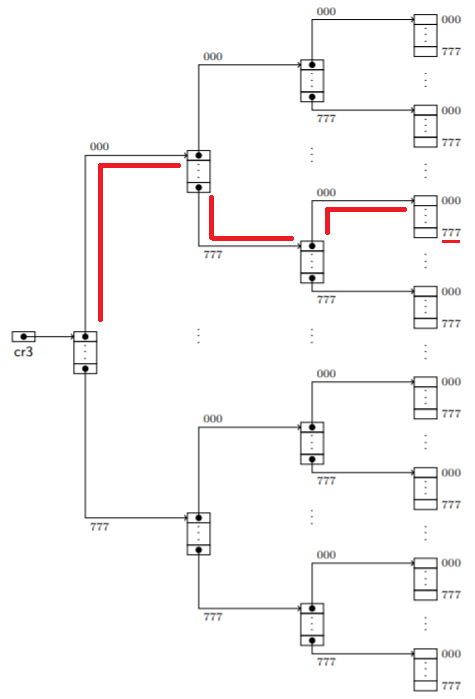
\includegraphics[scale=.8]{img/232.PNG}
\end{center}
\end{framed} 
\clearpage 
\subsection{Esempio non vitale: creazione di un albero di traduzione in Assembler}
Proviamo a creare un albero di traduzione (non per usarlo, solo per capire come si ragiona all'avvio): vogliamo mappare .
Lo facciamo in Assembler.

\subsubsection{Codice Assembler}
\scriptsize
\begin{multicols}{2}
\begin{verbatim}
	# vogliamo mappare i primi 8 MiB in se stessi
	#                          12
	# +--------------------------+-----------------+
	# |    n. frame              |          DAwdSWP|
	# +--------------------------+-----------------+
	
	.global setup_vm
	setup_vm:
	    # 0 -> 0
	    #  4   3   2   1   off
	    # 000 000 000 000 xywz -> 000 000 000 000 xywz
	    movq $tab3, tab4
	    movb $0b00000111, tab4
	
    	movq $tab2, tab3
	    movb $0b00000111, tab3
	
	    movabs $tab2, %rsi
	    movabs $tab1_0, %rdi
	    xor %rax, %rax
	
	.Loop0:
	    mov %rdi, (%rsi)
	    movb $0b00000111, (%rsi)
	    xor %rcx, %rcx
	.Loop1:
	    mov %rax, (%rdi, %rcx, 8)
	    movb $0b00000111, (%rdi, %rcx, 8)
	    add $0x1000, %rax
	    cmp $511, %rcx
	    jge .Lnext
	    inc %rcx
	    jmp .Loop1
	.Lnext:
	    cmp $tab1_3, %rdi
	    je .Lend
	    add $4096, %rdi
	    add $8, %rsi
	    jmp .Loop0
	.Lend:	
    	movabs $tab4, %rax
    	mov %rax, %cr3
	
    	ret
	
	.global a_page_fault
	a_page_fault:
	    pop %rdi
	    mov (%rsp), %rsi	
	    mov %cr2, %rdx
	    call c_page_fault
	    hlt
	
	.data
	.global tab4, tab3, tab2, tab1_0, tab1_1, tab1_2, tab1_3, tab1_4
	.balign 4096
	tab4:
	    .space 4096, 0
	tab3:
	    .space 4096, 0
	tab2:
	    .space 4096, 0
	tab1_0:
	    .space 4096, 0
	tab1_1:
	    .space 4096, 0
	tab1_2:
	    .space 4096, 0
	tab1_3:
	    .space 4096, 0
	tab2_3:
	    .space 4096, 0
	tab1_4:
	    .space 4096, 0
\end{verbatim}
\end{multicols}
\small
\begin{itemize}
	\item \textbf{Allocazione dello spazio per l'albero}.
	\begin{itemize}
		\item Ci serve spazio per un albero di traduzione.
		\item La tabella non può essere allocata ovunque, deve essere posta a un indirizzo che è multiplo di 4096. Facciamo questo con la seguente istruzione
		\begin{verbatim}
			.balign 4096
		\end{verbatim}
		\item \textbf{Quante tabelle di livello quattro ci servono?} 
		
		Una, visto che abbiamo solo la radice dell'albero.
		\item \textbf{Quante tabelle di livello tre ci servono?} Sempre una. 
		\begin{itemize}
			\item Ogni riga copre $1\,\text{GB}$.
			\item Se moltiplico per il numero di righe otteniamo
			\[512 \cdot 1\,\text{GB} = 512\,\text{GB}\]
			per $8\,\text{MB}$ basta una sola tabella.
		\end{itemize}
		\item \textbf{Quante tabelle di livello due ci servono?} Sempre una. 
		\begin{itemize}
			\item Ogni riga copre $2\,\text{MB}$.
			\item Se moltiplico per il numero di righe ottengo
			\[2\,\text{MB} \cdot 512 = 1\,\text{GB}\]
			Anche in questo caso una sola tabella è più che sufficiente.
		\end{itemize}
		\item \textbf{Quante tabelle di livello $1$ ci servono?} Quattro.
		\begin{itemize}
			\item Ogni riga copre $4\,\text{KB}$
			\item Se moltiplico per il numero di righe ottengo
			\[4\,\text{KB} \cdot 512 = 2048\,\text{KB} \]
			Questa volta non ci basta una sola tabella, ne servono $4$.
		\end{itemize}
	\end{itemize}
	Codice con cui allochiamo lo spazio 
	\begin{multicols}{2}
	\begin{verbatim}
			.data
		.global tab4, tab3, tab2, tab1_0, 
		tab1_1, tab1_2, tab1_3, tab1_4
		.balign 4096
		tab4:
		.space 4096, 0
		tab3:
		.space 4096, 0
		tab2:
		.space 4096, 0
		tab1_0:
		.space 4096, 0
		tab1_1:
		.space 4096, 0
		tab1_2:
		.space 4096, 0
		tab1_3:
		.space 4096, 0
		tab2_3:
		.space 4096, 0
		tab1_4:
		.space 4096, 0
	\end{verbatim}
\end{multicols}
	\item \textbf{Prepariamo l'albero}. 
	\begin{itemize}
		\item Dobbiamo pensare a come la MMU lo percorrerà (prende il numero di pagina, $0$, tralasciando l'offset). 
		\item Dobbiamo considerare, nei vari passaggi, la presenza di altre informazioni oltre al numero di frame: P, R/W, U/S, PCD, PWT, A, D. Alcuni di questi bit devono essere gestiti per forza, altrimenti non possiamo fare le nostre operazioni: settiamo i primi tre bit meno significativi (P, R/W, U/S). Lo facciamo aggiornando, di 64 bit, i 16 meno significativi
		\begin{verbatim}
			movb $0b00000111, tabX
		\end{verbatim}
		\item La prima riga di \emph{tab4} deve puntare \emph{tab3}, la prima riga di \emph{tab3} deve puntare a \emph{tab2}. 
		\begin{verbatim}
			movq $tab3, tab4
			movb $0b00000111, tab4
			
			movq $tab2, tab3
			movb $0b00000111, tab3
		\end{verbatim}
		\item Le righe di \emph{tab2} devono puntare alle tabelle di livello $1$. La cosa più conveniente è aggiornare le tabelle di livello $1$ attraverso dei cicli. 
		\begin{itemize}
			\item Le tabelle di livello $1$ sono una dopo l'altra, dunque non è necessario gestirle in modo distinto: si parte dalla prima riga della prima tabella di livello $1$ e si scorre tutto insieme.
			\item I parametri in ingresso sono due:
			\begin{itemize}
				\item registro RSI, indirizzo della tabella di livello $2$ \emph{tab2};
				\item registro RDI, indirizzo della prima riga della prima tabella di livello $1$.
			\end{itemize}
			\item Abbiamo due cicli annidati.
		\end{itemize}
		
	\end{itemize}
	\item \textbf{Aggiornamento di CR3}.
	
	Dopo aver riempito tutte le entrate di tutte le tabelle di livello $1$ possiamo mettere l'indirizzo dell'unica tabella di livello 4, \emph{tab4}, nel registro CR3. Da questo punto in poi non stiamo più utilizzando la traduzione preparata dal bootloader, ma la nostra.
	\begin{verbatim}
		movabs $tab4, %rax
		mov %rax, %cr3
	\end{verbatim}	
\end{itemize}
\normalsize 

\subsubsection{Codice C++} 
\small
\begin{verbatim}
	#include <libce.h>
	
	int var;
	
	extern "C" void setup_vm();
	extern "C" void a_page_fault();
	extern "C" natq tab4[], tab3[], tab2[], tab1_0[], tab1_1[], tab1_2[], tab1_3[], tab1_4[];
	extern "C" void c_page_fault(natq errore, natq rip, natq addr) {
    printf("errore %x, rip %x, addr %x\n", errore, rip, addr);
	}
	
	int main() {
     gate_init(14, a_page_fault);
     var = 1;
	    	printf("var = %d\n", var);
	    	pause();
	    	setup_vm();
	    	
	    	int *p = (int *)((natq)&var - 0x20f000 + 0x400000);
	    	printf("tab4[0] = %x\n", tab4[0]);
	    	printf("tab3[0] = %x\n", tab3[0]);
	    	printf("tab2[1] = %x\n", tab2[1]);
	    	printf("tab1_1[15] = %x\n", tab1_1[15]);
	    	
	    	printf("percorso alternativo:\n");
	    	printf("tab2[2] = %x\n", tab2[2]);
	    	printf("tab1_2[0] = %x\n", tab1_2[0]);
	    	*p = 2;
	    	printf("p %x, var = %d\n", p, var);
	    	printf("tab4[0] = %x\n", tab4[0]);
	    	printf("tab3[0] = %x\n", tab3[0]);
	    	printf("tab2[1] = %x\n", tab2[1]);
	    	printf("tab1_1[15] = %x\n", tab1_1[15]);
	    	
	    	printf("percorso alternativo:\n");
	    	printf("tab2[2] = %x\n", tab2[2]);
	    	printf("tab1_2[0] = %x\n", tab1_2[0]);
	    	
	    	pause();
	}
\end{verbatim}
\begin{itemize}
	\item \textbf{Eccezione \emph{page$\_$fault}}. 
	
	Immaginiamo di avere il seguente main
	\begin{verbatim} 
	int main() {
    var = 1;
    printf("var = %d\n", var);
    pause();
    setup_vm();
    pause();
}			
	\end{verbatim} 
Cosa succede dopo il secondo \emph{pause}? Si ha l'eccezione di tipo $14$ (\emph{page$\_$fault}), lanciata dalla MMU che non è riuscita a completare la traduzione. I motivi sono vari: incontra un bit $P=0$, scritture fallite perchè non è permessa la scrittura, o accessi ad aree di sistema in modalità utente...  Questa eccezione lascia in pila delle informazioni ulteriore: delle 4 quadword ci interessa quella in cima.
	\begin{itemize}
		\item Il bit meno significativo dice se l'errore è dovuto a una traduzione non valida ($0$) o a un errore di protezione ($1$).
		\item Il secondo bit meno significativo se l'eccezione è legata o meno a un'operazione di scrittura (si dice solo il tipo di operazione, non se era vietata la scrittura).
		\item Il terzo bit meno significativo segnala il livello di privilegio a cui si trovava il processore al momento dell'errore ($0$, sistema, $1$, utente). 
	\end{itemize} 
	Nel caso nostro abbiamo 
	
	\begin{center}
		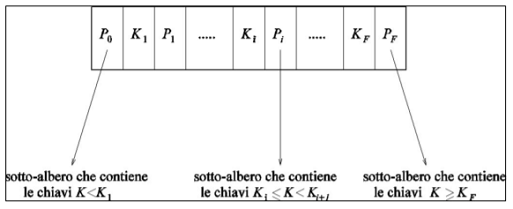
\includegraphics[scale=.8]{img/229.PNG}
	\end{center}
	L'errore è di traduzione, l'operazione era una scrittura in memoria
	\begin{verbatim}
		mov %edx, (%rax)
	\end{verbatim}
	\item \textbf{Registro CR2}.
	
	La MMU, quando non riesce a tradurre un indirizzo, scrive l'indirizzo che stava cercando di tradurre nel registro CR2.
	
	\item \textbf{Funzione da associare all'eccezione di tipo $14$}.
	
	Abbiamo scritto una routine da lanciare in caso di \emph{page$\_$fault}, come al solito divisa in due parti. La prima si trova nel codice Assembler visto prima e raccoglie i parametri in ingresso a partire dal contenuto della pila (ricordiamo che sono state poste delle informazioni in pila).
	\begin{itemize}
		\item RDI: quadword \emph{errore} (il codice identificativo dell'errore, che si trova in cima alla pila)
		\begin{verbatim}
		pop %rdi
		\end{verbatim} 
		\item RSI: quadword \emph{rip}, il rip dell'istruzione che il processore stava eseguendo quando si è manifestato il \emph{page fault}.
		\begin{verbatim}
			mov (%rsp), %rsi
		\end{verbatim}
		\item RDX: quadword \emph{addr}, contenuto del registro CR2 (l'indirizzo che la MMU non è riuscita a tradurre)
		\begin{verbatim}
			mov %cr2, %rdx
		\end{verbatim}
	\end{itemize}
	 La seconda parte, in C++, richiede la stampa delle informazioni sull'eccezione
	 \begin{verbatim}
extern "C" void c_page_fault(natq errore, natq rip, natq addr) {
    printf("errore %x, rip %x, addr %x\n", errore, rip, addr);
}
	 \end{verbatim}
 Associo la funzione al tipo $14$ con la \emph{gate$\_$init}
 \begin{verbatim}
gate_init(14, a_page_fault);
 \end{verbatim}
L'output ottenuto è il seguente
\begin{center}
	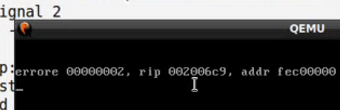
\includegraphics{img/231.PNG}
\end{center}

L'indirizzo a cui l'istruzione stava tentando di accedere è \emph{fec00000}. La traduzione di questo indirizzo virtuale non l'abbiamo creata: facciamolo!

\item 	\textbf{Aggiunta di una nuova traduzione di indirizzo}.

 Traduciamolo in se stesso: la \emph{libce} pensava di utilizzare indirizzi fisici, la sua intenzione era di scrivere proprio a quell'indirizzo. Il codice Assembler viene aggiunto in \emph{setup$\_$vm}, dopo l'etichetta \emph{Lend}.
\begin{multicols}{2}
\begin{verbatim}
		# tab4
	# 0: -> tab3
	#       0: -> tab2
	#             0: tab1_0
	#             1: tab1_1
	#             2: tab1_2
	#             3: tab1_3
	#       3: -> tab2_3
	#             766: -> tab1_4
\end{verbatim}
\columnbreak
\begin{verbatim}
	#	
	# fec00000 -> fec00000
	# 
	#   numero di pagina
	#
	# 000000000 000/000/011 111/110/110 000/000/000
	# 000       003         766         000
	#
	#
\end{verbatim}
\end{multicols}
\begin{verbatim}	
	movl $tab2_3, tab3 + 8*3
	movb $0b00000111, tab3 + 8*3
	
	movl $tab1_4, tab2_3 + 0766 * 8 <--- 0766 interpretato in base 8
	movb $0b00000111, tab2_3 + 0766 * 8 <--- 0766 interpretato in base 8
	
	movl $0xfec00000, tab1_4
	movb $0b00001111, tab1_4
\end{verbatim}
\begin{itemize}
		\item Scomponendo l'indirizzo in ottave capiamo meglio come muoverci.
		\item Siamo in \emph{tab4}. Passiamo a \emph{tab3} attraverso la prima entrata dell'unica tabella.
		\item Siamo in \emph{tab3}: l'entrata che ci interessa è la terza, dunque abbiamo una nuova tabella da creare rispetto a prima (\emph{tab2$\_$3}).
		\item Nella tabella appena creata ci interessa la $502-$esima entrata. Attraverso questa si passa alla tabella \emph{tab1$\_$4} (ulteriore tabella in più).
		\item Le istruzioni mov per aggiornare il contenuto dell'albero le abbiamo già viste nella preparazione dell'albero. Si tenga solo conto che avendo l'APIC a quell'indirizzo conviene disattivare la cache: segue il settaggio del quarto bit meno significativo nelle varie \emph{movb}.
\end{itemize}
\item \textbf{Creazione di un nuovo indirizzo virtuale per la variabile \emph{var}}.

Creiamo una variabile \emph{var} nel nostro programma.
\begin{center}
	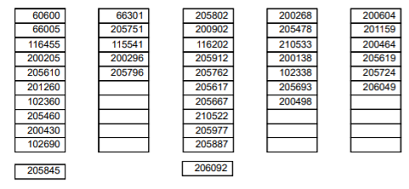
\includegraphics{img/230.PNG}
\end{center}
Siamo sicuri, per quello che abbiamo fatto prima, che già esista un indirizzo virtuale. Mappiamo un altro indirizzo virtuale, completamente diverso, nello stesso indirizzo fisico. Il codice Assembler viene aggiunto in \emph{setup$\_$vm}, dopo l'etichetta \emph{Lend}.
\begin{verbatim}
	# 0x400-000 -> 0x20f-000
	#
	#  numero di pagina
	# 
	# 000000000 000000000 000000010 000000000
	# 000       000       002       000
	
	movl $0x20f000, tab1_2
	movb $0b0000111, tab1_2
\end{verbatim}
A livello di tabelle abbiamo già tutto, non ci serve fare altro. Entrata $0$ in \emph{tab4}, Ci interessano le seguenti entrate: entrata $0$ in \emph{tab3}, entrata $2$ in \emph{tab2}, entrata 0 in \emph{tab1$\_$2}. 

A questo punto possiamo vedere, nel \emph{main}, l'utilizzo di questo nuovo indirizzo virtuale: la variabile \emph{var} viene modificata attraverso il puntatore \emph{p} (che contiene il nuovo indirizzo virtuale)
\begin{verbatim}
	int *p = (int *)((natq)&var - 0x20f000 + 0x400000);
	*p = 2;
	printf("p %x, var = %d\n", p, var);
\end{verbatim}

\item \textbf{Modifica delle tabelle dell'albero in C++}.

Possiamo notare come nel \emph{main} si recuperi diverse volte il contenuto delle tabelle dell'albero. Possiamo agire sulla tabella a partire dal C++, dopo aver definito il tipo. Nella lezione successiva è presente un esempio di scrittura (col cosiddetto \emph{Page Size Flag}).
\end{itemize}
\normalsize 

\section{Pagine di dimensione diversa (\emph{Page Size} flag)}
Abbiamo introdotto il trie, che ci offre il vantaggio di non avere sottoalberi se relativi indirizzi non sono utilizzati. Altra cosa utile è la possibilità di creare \textbf{pagine di dimensione diversa}.

\paragraph{Struttura indirizzo virtuale} Abbiamo:
\begin{itemize}
	\item 12 bit di offset (bit meno significativi);
	\item numero di pagina spezzato in quattro indici.
\end{itemize}
Più la pagina è grande, più è grande l'offset e piccolo il numero di pagina. 
\paragraph{Proposta} Se la dimensione delle pagine è variabile allora si potrebbe aumentarne la dimensione, arrivando a ridurre di $1$ i livelli dell'albero (velocità della traduzione - tre accessi invece di quattro - e minore spazio occupato dalla struttura dati). La cosa solitamente non succede perchè pagine di dimensioni più elevate possono comportare un maggiore spreco di memoria (si consideri che la pagina è unità di condivisione tra progetti, e di condivisione).

\paragraph{\emph{Page Size} flag} Nonostante questo l'albero ci permette di non dover decidere a priori la grandezza, possiamo decidere in modo flessibile. Questo perchè all'interno di ogni entrata abbiamo un flag \textbf{Page Size} (PS) che dica alla MMU che in questo percorso (supponiamo di settare il flag al livello $2$) la pagina è più grande (si indica che il percorso finisce lì, nell'esempio detto abbiamo una dimensione di $2\,\text{MB}$). Il set o meno di questo flag determina il numero di bit del numero di pagina all'interno dell'indirizzo virtuale.
\begin{itemize}
	\item \textbf{Vantaggio}: ci servono meno tabelle per fare la traduzione identità (quella dove indirizzi virtuali corrispondono a indirizzi fisici, nella parte di RAM riservata al sistema).
\end{itemize}

\subsection{Esempio di utilizzo del flag nell'ultimo esempio di esercizio}
Riprendiamo l'esercizio della scorsa lezione, abbiamo visto che possiamo leggere le tabelle dell'albero dal C++, dopo aver definito il tipo. Avevamo creato una traduzione (identità) solo fino a $8\,\text{MB}$, questo significa che se dichiaro qualcosa fuori da questa regione viene lanciata un'eccezione (per $P=0$).
\paragraph{Cosa vogliamo fare?} Adesso vogliamo creare una traduzione identità per altri $2\,\text{MB}$: senza le cose appena introdotte risulterebbe necessario introdurre una nuova tabella. Ci limitiamo a fare
\begin{verbatim}
	tab2[4] = 0x800000 | 0x87;
\end{verbatim}
settando il bit più significativo del byte di accesso, il bit PS. In questo modo diciamo ad MMU che la traduzione è già finita quando si arriva a questa entrata.


\section{Cache \emph{Translation Lookaside Buffer} (TLB)}
Dal punto di vista dell'hardware ci resta un'unica cosa. L'implementazione via trie è comoda ma presenta anche degli svantaggi: pensiamo al numero elevato di accessi (con questi alberi il numero di accessi moltiplica ogni volta\footnote{La cosa può avere grande impatto sul tempo di esecuzione di un programma: prelievo delle istruzioni, prelevo o scrittura degli operandi che si trovano in memoria...}). Anche accedere in cache ha un costo: il singolo accesso non occupa centinaia di clock, ma rispetto a prima abbiamo un numero maggiore di accessi in cache. 
\paragraph{Soluzione} La soluzione è la \emph{Translation Lookaside Buffer} (TLB), una cache dedicata alla MMU (una cache delle traduzioni, entro qua per non consultare il trie). 
\paragraph{Cache} Limitiamoci a parlare delle cache a $4\,\text{KB}$: la cache conterrà le entrate delle tabelle di livello $1$. La TBL è una letteralmente una cache a 8/16 vie. Lo schema interno è quasi del tutto identico a quello già visto.
\begin{center}
	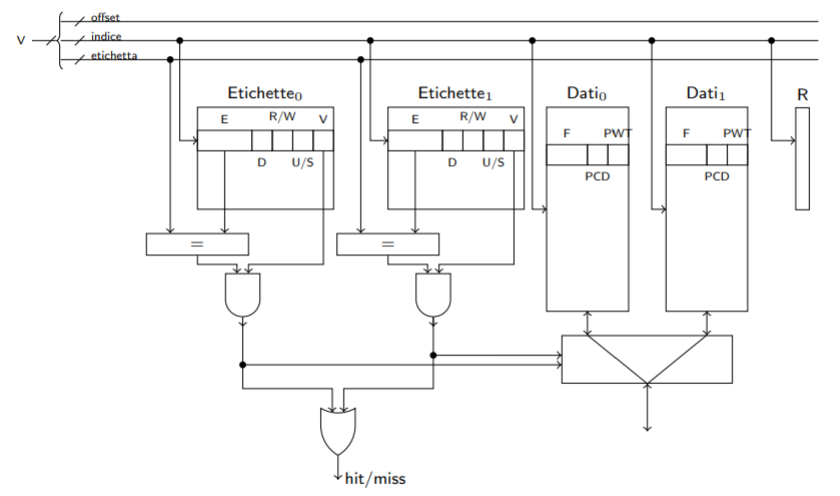
\includegraphics[scale=.8]{img/228.PNG}
\end{center}
Viene memorizzata l'associazione tra numero di pagina e numero di frame, oltre alle informazioni poste nel descrittore di pagina.

\paragraph{Osservazione su alcuni bit} 
\begin{itemize}
	\item Abbiamo detto che una pagina è riservata al sistema se tutti i bit U/S (uno per livello) sono settati. Che informazione metto nel TLB (1 bit) affinchè il controllo possa essere equivalente a quello fatto sul trie (4 bit))?
	La AND dei vari bit incontrati.
	\item Il bit A indica che c'è stato un accesso: non è riportato nel TLB perchè se l'entrata è presente in cache è logico che c'è stato un accesso.
	\item La cosa è più complessa col bit D: può accadere che su una data pagina ho inizialmente una lettura e poi una scrittura. In queste condizioni non ce ne accorgiamo passando dalla cache: $D$ rimane a zero nonostante la scrittura. {Risolviamo così: in caso di hit con operazione di scrittura e $D$ a zero non si concede immediatamente la scrittura (\emph{miss}), ma si ripercorre il trie}.   
	\item Il bit $P$ non è presente: se abbiamo riportato l'entrata nella cache significa che abbiamo trovato tutti i $P=1$.
	\item Se $V=0$ la riga non è significativa (è il bit già incontrato quando abbiamo spiegato la cache, non ha a che vedere con le entrate delle tabelle del trie)
\end{itemize}
\subsection{Riprendiamo l'esempio di esercizio} Abbiamo visto che è possibile modificare la variabile \emph{var} a partire da due indirizzi virtuali completamente diversi. Immaginiamo di avere il seguente main
\begin{verbatim}
	#include <libce.h>
	#include <vm.h> <----  novita'
	int var;
	
	extern "C" void setup_vm();
	extern "C" void a_page_fault();
	extern "C" natq tab4[], tab3[], tab2[], tab1_0[], tab1_1[], tab1_2[], tab1_3[], tab1_4[];
	extern "C" void c_page_fault(natq errore, natq rip, natq addr) {
		    printf("errore %x, rip %x, addr %x\n", errore, rip, addr);
	}

int main() {
    gate_init(14, a_page_fault);
    var = 1;
    prinft(var = %d\n", var);
    pause();
    setup_vm();
    int *p = (int*)((natq)&var - 0x20f000 + 0x400000);
    tab1_2[0] = 0x20f000 | 0x07;
    *p = 2;
    printf("var = %d\n", var)
    pause();
}
\end{verbatim}
Se compiliamo vediamo di nuovo lo scrivere in \emph{var} attraverso un indirizzo virtuale alternativo. 
\begin{center}
	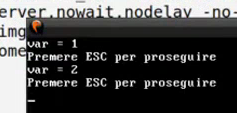
\includegraphics{img/233.PNG}
\end{center}
Aggiungiamo la seguente riga prima della scrittura in \emph{tab1$\_$2}.
\begin{verbatim}
	*p = 3;
\end{verbatim}
 Stavolta \emph{var} non viene modificato, l'output da $1$.
\begin{center}
	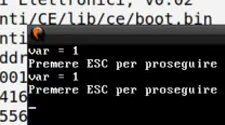
\includegraphics{img/234.PNG}
\end{center}
\paragraph{Come mai?} 
\begin{itemize}
	\item Inizialmente l'indirizzo \emph{0x400000} è mappato su se stesso. 
	\item Con la prima modifica
	\begin{verbatim}
	*p = 3
	\end{verbatim}
	agiamo sull'indirizzo fisico \emph{0x400000}. Segue che non modificheremo \emph{var} con questa istruzione.
	\item Con la seconda modifica, che avviene dopo l'aggiornamento della riga di \emph{tab1$\_$2}
	\begin{verbatim}
		*p = 2;
	\end{verbatim} La traduzione nel trie è ancora quella vecchia: abbiamo agito sempre su \emph{0x400000}, e non su \emph{var}.
	\item Non è la cache della memoria il problema, \textbf{ma la traduzione che ha usato la MMU}.
\end{itemize}
Questo problema è dovuto alla cache TLB. Il problema è il solito: mantenere la consistenza a seguito di modifiche. Quando modifico una traduzione il TLB quasi sicuramente non se ne accorge. Dobbiamo invalidarlo in modo esplicito! Possiamo farlo in due modi.
\begin{enumerate}
	\item \textbf{Istruzione mov con registro CR3 operando destinatario}
	\begin{verbatim}
		movq %rax, %cr3
	\end{verbatim}
	L'istruzione può potenzialmente alterare tutta la tabella di livello $4$, quindi tutte le informazioni contenute nel TLD non possono considerarsi più valide. 
	\item \textbf{Istruzione Assembler \emph{invlpg} (\emph{invalid page})}
	\begin{verbatim}
		invlpg operando_in_memoria
	\end{verbatim}
	L'istruzione permette di invalidare la traduzione relativa all'indirizzo passato come operando. La libreria \emph{libce},  \emph{vm.h}, offre una funzione già pronta per poter eseguire l'istruzione da C++: \textbf{invalida$\_$entrata$\_$TLB}.
	\begin{center}
		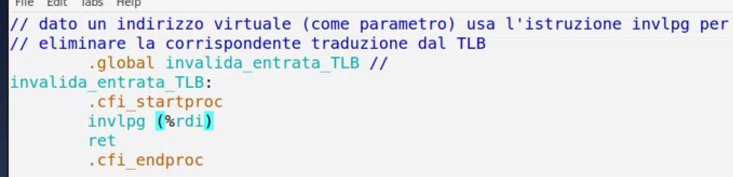
\includegraphics[scale=.8]{img/235.PNG}
	\end{center} 
\end{enumerate}
A questo punto torniamo sul \emph{main} e scriviamolo così
\begin{verbatim}
int main() {
    	gate_init(14, a_page_fault);
    	var = 1;
    	prinft(var = %d\n", var);
    	pause();
    	setup_vm();
    	int *p = (int*)((natq)&var - 0x20f000 + 0x400000);
    	
    	*p = 3; <--- riga in piu'
    	
    	tab1_2[0] = 0x20f000 | 0x07;
    	
    	invalida_entrata_TLB(p); <--- riga in piu'
    	
    	*p = 2;
    	printf("var = %d\n", var)
    	pause();
}
\end{verbatim}
	L'output torna e la seconda modifica del contenuto puntato da \emph{p} ha agito su \emph{var}.




\chapter{Implementazione della paginazione}

\section{Extra: \emph{typedef} per indirizzi fisici e virtuali} Nel file \emph{tipo.h} della \emph{libce} sono presenti due ulteriori typedef per distinguere indirizzi fisici da indirizzi virtuali (solo comodità visiva, sono entrambi \emph{unsigned long})!
\begin{itemize}
	\item \begin{verbatim}typedef unsigned long vaddr;\end{verbatim}
	Indirizzi virtuali
	\item \begin{verbatim}typedef unsigned long paddr;\end{verbatim}
	Indirizzi fisici
\end{itemize}
Sono molto utilizzati nelle funzioni di \emph{vm.h}. In quest'ultimo file troviamo anche 
\begin{itemize}
	\item \begin{verbatim}typedef natq tab_entry;
	\end{verbatim}
	che usiamo per le entrate delle tabelle delle pagine.
\end{itemize} 
\section{Costanti in \emph{vm.h} della \emph{libce}}
\subsection{Numero massimo di livelli del \emph{trie}} \begin{verbatim}
		static const int MAX_LIV = 4;
	\end{verbatim}
	Numero di livelli massimo. Nel nostro codice abbiamo $4$, ma con processori a $57$ bit è possibile avere un livello in più. 
\subsection{Maschere}
\begin{itemize}
	\item 
	\begin{verbatim}
		static const natq BIT_SEGNO = (1ULL << (12 + 9* MAX_LIV -1)); <- ULL unsigned long long
	\end{verbatim}
	Calcoliamo il bit dove si trova il segno (l'ultimo bit più significativo che ci interessa). Si pone ULL per evitare problemi con lo shift. La maschera è utile nella funzione per la normalizzazione degli indirizzi. Nel caso nostro avremo:
	\begin{verbatim}
		BIT_SEGNO = (1ULL << 47);
	\end{verbatim}
	\item \begin{verbatim} 
		static const natq MASCHERA_MODULO = BIT_SEGNO - 1;
	\end{verbatim} 
	Maschera con cui recupero il modulo.
\end{itemize}	
\subsection{Costanti per la manipolazione dei descrittori di pagina e di tabella}
\small
\begin{verbatim}
	const natq BIT_P    = 1U << 0; // il bit di presenza
	const natq BIT_RW   = 1U << 1; // il bit di lettura/scrittura
	const natq BIT_US   = 1U << 2; // il bit utente/sistema
	const natq BIT_PWT  = 1U << 3; // il bit Page Wright Through
	const natq BIT_PCD  = 1U << 4; // il bit Page Cache Disable
	const natq BIT_A    = 1U << 5; // il bit di accesso
	const natq BIT_D    = 1U << 6; // il bit "dirty"
	const natq BIT_PS   = 1U << 7; // il bit "page size"
	
	const natq ACCB_MASK  = 0x00000000000000FF; // maschera per il byte di accesso
	const natq ADDR_MASK  = 0x7FFFFFFFFFFFF000; // maschera per l'indirizzo
\end{verbatim}
\normalsize

\section{Funzioni in \emph{vm.h} della \emph{libce}}
Il file è incluso attraverso apposita direttiva in \emph{sistema.cpp}, precisamente nella sezione dedicata alla paginazione
\begin{verbatim}
#include <vm.h>
\end{verbatim}
\subsection{Normalizzazione dell'indirizzo con \emph{norm}}
\small 
\begin{verbatim}
static inline vaddr norm(vaddr a) {
    return (a & BIT_SEGNO) ? (a | ~MASCHERA_MODULO) : (a & MASCHERA_MODULO);
}
\end{verbatim}
\normalsize 
%\begin{center}
%	\includegraphics{img/236.PNG}
%\end{center} 
\begin{itemize}
	\item Dato un indirizzo virtuale la funzione restituisce la corrispondente versione normalizzata (i $16$ bit più significativi sono uguali al $47-$esimo bit dell'indirizzo).
	\item Step:
	\begin{itemize}
		\item Controlliamo il bit di segno.
		\item Se è uguale ad $1$ metto i bit più significativi rimanenti uguali ad $1$
		\item Se è uguale a 0 metto  i bit più significativi rimanenti uguali a $0$.
	\end{itemize}
\end{itemize}
\subsection{Grandezza di una regione con \emph{dim$\_$region}}
\small 
\begin{verbatim}
static inline constexpr natq dim_region(int liv) {
    natq v = 1ULL << (liv * 9 + 12);
    return v;
}
\end{verbatim}
\normalsize 
%\begin{center}
%	\includegraphics{img/237.PNG}
%\end{center} 
\paragraph{Definizione} Con \emph{regione di livello liv} intendiamo l'intervallo di indirizzi coperti da una singola entrata di una tabella di livello $i+1$. Questo significa che:
\begin{itemize}
	\item una regione di livello $0$ è grande $4096\,\text{byte}$;
	\item una regione di livello $1$ è grande $2\,\text{MiB}$;
	\item una regione di livello $3$ è grande $1\,\text{GiB}$.
\end{itemize}
\paragraph{Scopo della funzione} La funzione ci restituisce la grandezza di una regione di livello \emph{liv}: prendo $12$ (numero di bit dell'offset) e mi ricordo che ogni livello è rappresentato da $9$ bit, quindi sommo a $12$ il prodotto tra $9$ e \emph{liv}. Concludiamo traslando
\[1 \cdot 2^{\text{liv} \cdot 9 + 12}\]

\subsection{Funzioni \emph{base} e \emph{limit} per l'indirizzo di base di una regione}
\small 
\begin{verbatim}
static inline vaddr base(vaddr v, int liv) {
    natq mask = dim_region(liv) - 1;
    return v & ~mask;
}

static inline vaddr limit(vaddr e, int liv) {
    natq dr = dim_region(liv);
    natq mask = dr - 1;
    return (e + dr - 1) & ~mask;
}
\end{verbatim}
\normalsize 
%\begin{center}
%	\includegraphics{img/238.PNG}
%\end{center} 
%\begin{center}
%	\includegraphics{img/239.PNG}
%\end{center} 
Dato un indirizzo virtuale \emph{v} le due funzioni restituiscono un altro indirizzo virtuale. Precisamente:
\begin{itemize}
	\item la funzione \emph{base} restituisce la base della pagina di livello \emph{liv} in cui cade l'indirizzo \emph{v};
	\begin{itemize}
		\item Otteniamo il numero di regione mascherando i bit meno significativi dell'indirizzo. Vediamo un esempio semplificato
		\[0b1000 - 0b0001 = 0b0111 \longrightarrow \,!(0b0111)=0b1000\]
		Se uso l'operatore AND spariscono i tre bit meno significativi.
	\end{itemize}
	\item la funzione \emph{limit} restituisce la base della prima regione di livello \emph{liv} a destra dell'intervallo (quello della regione dove si trova l'indirizzo \emph{v}).
	\begin{itemize}
		\item Recupero la dimensione di una regione di livello \emph{liv}.
		\item  Decremento per ottenere una maschera (bit più significativo uguale a $0$, tutti gli altri uguali ad $1$).
		\item Sommo all'indirizzo \emph{e} la dimensione della regione e decremento di $1$. A quel punto faccio AND con la negazione della maschera \emph{mask} (mi sbarazzo dei bit meno significativi).
	\end{itemize}
\end{itemize}

\subsection{Funzioni per lavorare sul \emph{trie}}

\subsubsection{Estrazione dell'indirizzo fisico da un'entrata (\emph{extr$\_$IND$\_$FISICO})}
\small 
\begin{verbatim}
static inline paddr extr_IND_FISICO(tab_entry descrittore) {
    return descrittore & ADDR_MASK;
}
\end{verbatim}
\normalsize 
%\begin{center}
%	\includegraphics{img/240.PNG}
%\end{center} 
La funzione mi permette di ottenere l'indirizzo fisico presente nella \emph{tab$\_$entry} indicata nei parametri di ingresso. Nel caso della foglia non restituiremo solo un indirizzo fisico, ma l'indirizzo della base del frame.
\paragraph{Cosa faccio} Mi ricordo dove è collocato l'indirizzo fisico all'interno del descrittore, tenendo conto che l'offset (i primi $12$ bit) è sempre una sequenza di zeri. Utilizzo la costante \emph{ADDR$\_$MASK}, già vista
\begin{verbatim}
	const natq ADDR_MASK  = 0x7FFFFFFFFFFFF000;
\end{verbatim}
\subsubsection{Settaggio dell'indirizzo fisico in un'entrata (\emph{set$\_$IND$\_$FISICO})}
\small 
\begin{verbatim}
static inline void set_IND_FISICO(tab_entry& descrittore, paddr ind_fisico) {
    descrittore &= ~ADDR_MASK;
    descrittore != ind_fisico & ADDR_MASK;
}
\end{verbatim}
\normalsize 
%\begin{center}
%	\includegraphics{img/241.PNG}
%\end{center} 
Setto l'indirizzo fisico nel descrittore con due step:
\begin{itemize}
	\item resetto tutti i bit relativi all'indirizzo fisico;
	\item imposto i bit ponendo il nuovo indirizzo fisico (metto l'indirizzo nel descrittore con un OR, dopo aver rimosso l'offset con l'AND).
\end{itemize}
Anche qua utilizziamo la costante \emph{ADDR$\_$MASK}
\begin{verbatim}
	const natq ADDR_MASK  = 0x7FFFFFFFFFFFF000;
\end{verbatim}

\subsubsection{Indice dell'entrata di un vaddr in una tabella di livello \emph{liv}	 (\emph{i$\_$tab})}
\small 
\begin{verbatim}
static inline int i_tab(vaddr ind_virt, int liv) {
    int shift = 12 + (liv - 1) * 9;
    natq mask = 0x1ffULL << shift;
    return (ind_virt & mask) >> shift;
}
\end{verbatim}
\normalsize 
%\begin{center}
%	\includegraphics{img/242.PNG}
%\end{center} 
Dato un indirizzo virtuale \emph{ind$\_$virt}, estraggo dall'indirizzo virtuale l'indice del descrittore relativo, in una tabella di livello \emph{liv}.
\begin{itemize}
	\item Prendo una maschera di $9$ bit, che shifto in modo da posizionarla sotto l'indice che mi interessa.
	\item Applico la maschera con l'operatore AND e shifto nuovamente per portare l'indice sulle cifre meno significative.
\end{itemize}

\subsubsection{Indirizzo di un'entrata di indice \emph{index} da una tabella \emph{tab} (\emph{get$\_$entry})}
\small
\begin{verbatim}
static inline tab_entry& get_entry(paddr tab, natl index) {
    tab_entry *pd = reinterpret_cast<tab_entry*>(tab);
    return pd[index];
}
\end{verbatim}
\normalsize 
%\begin{center}
%	\includegraphics{img/243.PNG}
%\end{center} 
Dato l'indirizzo fisico di una tabella \emph{tab} e un indice \emph{index}, la funzione restituisce il riferimento a una certa entrata.

\subsubsection{Classe \emph{tab$\_$iter} per la visione del trie (iteratore)}
Una cosa che si deve fare molto spesso è visitare l'albero. Uno, per esempio, potrebbe essere interessato a visitare tutte le entrate che si occupano della traduzione degli indirizzi in un certo intervallo di indirizzi. Le strade possibili sono due:
\begin{enumerate}
	\item scrivere una funzione ricorsiva;
	\item realizzare un \emph{iteratore} (cioè un qualcosa che si ricorda in che punto siamo arrivati nell'albero, e rimane lì finchè qualcuno non gli dice di spsotarsi).
\end{enumerate}
{La scelta adottata è la seconda}.
\paragraph{Codice}
\small
\begin{verbatim}
class tab_iter {
    struct stack {
        vaddr cur, end;
        paddr tab;
    } s[MAX_LIV + 1];
		
    int l;
		
    stack *sp() { return &s[l - 1]; }
    stack const *sp() const { return &s[l - 1]; }
		    stack *sp(int lvl) { return &s[lvl - 1]; }
		    stack *pp() { return &s[MAX_LIV]; }
		    bool done() const { return !sp()->tab; }
		
		    public:
		        static bool valid_interval(vaddr beg, natq dim) {
			            vaddr end = beg + dim - 1;
		            return !dim || (
			            // no wrap-around
			            !(end < beg)
			            // non inizia nel buco
			            &&   norm(beg) == beg
			            // non termina nel buco
			            &&   norm(end) == end
			            // non attraversa il buco
			            &&   !((beg & BIT_SEGNO) != (end & BIT_SEGNO)));
		        }
		
		        tab_iter(paddr tab, vaddr beg, natq dim = 1, int liv = MAX_LIV);
		
		        vaddr get_v() const {
			            return sp()->cur;
		        }
		
		        [... vedere le spiegazioni successive]
		        bool down();
		        bool up();
		        bool right();
		        void post();
		        void next_post();
	    };
\end{verbatim} 
\normalsize
\begin{itemize}
	\item L'iteratore viene costruito indicando:
	\begin{itemize}
		\item l'indirizzo fisico della tabella \emph{tab} (normalmente una tabella di livello $4$), 
		\item un indirizzo virtuale di partenza \emph{beg}  (di cui si vuole visitare la traduzione),
		\item quanto è grande l'intervallo di indirizzi virt. che si vuole visitare (\emph{dim}, di default $1$),
		\item il livello di partenza (di default \emph{MAX$\_$LIV}).
	\end{itemize} 
	\begin{verbatim}
		tab_iter(paddr tab, vaddr beg, natq dim = 1, int liv = MAX_LIV);
	\end{verbatim}
	\item L'operatore booleano indica "se la visita è finita", cioè se tutte le entrate coinvolte nella traduzione che va da \emph{beg} a \emph{beg + DIM} (quest'ultimo escluso) sono state visitate.
	\begin{verbatim}
		bool done() const { return !sp()->tab; }
		operator bool() const {
			return !done();
		}
	\end{verbatim}
	\item Con la funzione \emph{next} indichiamo all'iteratore di spostarsi sulla prossima entrata da visitare. Il tipo di visita è  \emph{anticipata}.
	\begin{verbatim}
		void next();
	\end{verbatim}
	\item Quando siamo fermi su un'entrata possiamo chiedere varie informazioni:
	\begin{itemize}
		\item a che livello siamo
		\begin{verbatim}
			int get_l() const {
				    return l;
			}
		\end{verbatim}
		\item se l'entrata è una foglia (ho $P=0$, ho livello $1$, oppure $PS$ è settato)
		\begin{verbatim}
			bool is_leaf() const {
				    tab_entry e = get_e();
				    return !(e & BIT_P) || (e & BIT_PS) || l == 1;
			}
		\end{verbatim}
		\item il riferimento all'entrata (in modo da poterlo modificare)
		\begin{verbatim}
			tab_entry& get_e() const {
				    return get_entry(sp()->tab, i_tab(sp()->cur, l));
			}
		\end{verbatim}
		\item l'indirizzo fisico della tabella che contiene l'entrata su cui l'iteratore è fermo 
		\begin{verbatim}
			paddr get_tab() const {
				    return sp()->tab;
			}
		\end{verbatim}
	\end{itemize}
\end{itemize}
\subsubsection{Esempio di uso della classe \emph{tab$\_$iter}} 
Partiamo dalla radice del nostro albero, \emph{tab4} (paddr), e scorre tutto l'intervallo che abbiamo mappato ($8\,\text{MB}$, da $0$ a $0x800000$).
\begin{verbatim}
for(tab_iter it((paddr)tab4, 0, 0x800000); it; it.next()) {
    flog(LOG_DEBUG, "tab %x, liv %d, entry %x", it.get_tab(), it.get_l(), it.get_e());
}
\end{verbatim}
L'output è il seguente
\begin{center}
	\includegraphics[scale=.85]{img/244.PNG}
\end{center} 
Si includa anche un richiamo alla funzione \emph{panic}, che non fa niente.
\begin{verbatim}
	extern "C" void panic();
\end{verbatim}

\normalsize 

\begin{framed}
\noindent \textbf{Recap}. Il modulo sistema si deve preoccupare di gestire sia la memoria fisica che quella virtuale.
\begin{itemize}
	\item \textbf{Memoria fisica}.
	
	Per quanto riguarda quella fisica (la RAM) abbiamo detto che una parte è ad uso esclusivo del modulo sistema (con sezioni \textit{text, data, stack, heap} del sistema), mentre la parte rimanente è divisa in frame. Si tenga conto che tutto ciò che è presente in questa seconda area di memoria non è tutta accessibile all'utente: gli indirizzi devono essere tradotti.
	\item \textbf{Memoria virtuale}.
	
	Il sistema deve creare gli spazi di indirizzamento di ogni singolo processo: abbiamo una serie di indirizzi (col solito buco). A priori decidiamo che tutti gli indirizzi che vanno da $0$ fino al buco appartengono al sistema (solo traduzioni con $U/S=0$, quindi accessibili solo se ci troviamo a livello sistema). La parte rimanente è accessibile a livello utente, contiene traduzioni utilizzabili a livello utente (e anche a livello sistema).
\end{itemize}
\end{framed}

\clearpage 

\section{Suddivisione dello spazio di indirizzamento}
	\paragraph{Sistema} La parte accessibile a livello sistema si divide in tre parti, ciascuna dedicata a priori a una certa cosa:
	\begin{itemize}
		\item una prima parte dedicata al \textit{modulo sistema} (unica parte con traduzione identità);
		\item una dedicata al \textit{modulo I/O};
		\item una dedicata alla \textit{pila sistema} (quella usata dal processore a livello sistema).
	\end{itemize}
	Nel modulo sistema garantiamo all'accesso a tutta la RAM, ma anche ad altre cose come l'APIC. Tutto il resto (modulo I/O, pila sistema e livello utente) conterrà traduzioni che portano ad $M2$.
	\paragraph{Utente}
	Il livello utente si divide in due parti:
	\begin{itemize}
		\item l'area con \emph{text, data, heap};
		\item pila utente.
	\end{itemize}
Le pagine sono mappate sempre in $M2$.
\begin{center}
	\includegraphics[scale=.6]{img/245.PNG}
\end{center}
\paragraph{Sono necessarie le traduzioni di modulo I/O e pila sistema?} 
\begin{itemize}
	\item Teoricamente non ci sarebbe bisogno di fare queste traduzioni: potrei utilizzare gli indirizzi della finestra, cioè quelli del modulo sistema.
	\item Conviene avere questa seconda traduzione. Abbiamo frame allocati dinamicamente: se il sistema ha già lavorato per un po' diventa molto improbabile che i frame relativi a un processo siano tutti consecutivi. Il mapping per pila e periferiche I/O permette di creare indirizzi contigui (anche se i frame non lo sono). 
\end{itemize} 






\paragraph{Processi concorrenti, mappaggio comune}
Pensiamo a un altro processo, anche lui con la sua memoria virtuale. Alcune traduzioni saranno esattamente identiche a quelle di $P1$:
\begin{itemize}
	\item modulo sistema
	\item modulo I/O
	\item \textit{text, data, heap} del livello utente (gli indirizzi sono gli stessi, ma hanno significato diverso a seconda del processo attivo\footnote{Quindi a seconda della traduzione attiva.}).
\end{itemize}
\paragraph{Attenzione} Alcune persone dicono all'esame che la MMU sceglie se usare la parte sopra o quella sotto in base al livello di privilegio. \textbf{Questa frase non ha alcun senso}: la MMU usa le traduzioni in base agli indirizzi ricevuti e controlla se il livello di privilegio è sufficiente per determinare l'accessibilità della traduzione. Non è un discorso di scegliere cosa usare.

%\paragraph{Cosa dobbiamo sapere?} L'utente, ribadiamo, non ha bisogno di sapere tante cose per scrivere un programma. Nel sistema, invece, dobbiamo ricordare:
%\begin{itemize}
%	\item dove si trova il codice che stiamo leggendo;
%	\item quali indirizzi stiamo usando;
%	\item quali sono le traduzioni attive al momento in cui il codice è stato eseguito.
%\end{itemize}
%Vediamo un esempio in cui è importante sapere queste cose.
%\paragraph{Scrivere nella pila sistema di un altro processo} Sia $P1$ il processo in esecuzione: esso invoca una primitiva di sistema che vuole scrivere qualcosa sulla pila sistema del processo $P2$. Come facciamo?
%\begin{itemize}
%	\item La prima cosa di cui siamo certi è che non utilizzeremo gli indirizzi virtuali della pila sistema, che riguardano il processo in esecuzione $P1$.
%\end{itemize}


\section{Costanti dedicate alla memoria virtuale}
Ritorniamo nel file \emph{include/costanti.h} per vedere alcune costanti legati alla memoria virtuale. Abbiamo detto che la suddivisione dello spazio di indirizzamento in varie parti è fatta a priori. La memoria virtuale è allocata in unità di regioni di livello $4$ (di $512\,\text{GB}$ alla volta). In sostanza decidiamo quante entrate della tabella di livello $4$ di ciascun processo sono dedicate a una cosa oppure a un'altra.
\begin{verbatim}
// tipo del driver del timer (priorità massima)
#define TIPO_TIMER		0xFF

// ( suddivisione della memoria virtuale
//   N    = Numero di entrate in root_tab
//   I	  = Indice della prima entrata in root_tab
//   SIS  = SIStema
//   MIO  = Modulo IO
//   UTN  = modulo UTeNte
//   C    = Condiviso
//   P    = Privato
#define I_SIS_C		0
#define I_SIS_P		1
#define I_MIO_C		2
#define I_UTN_C       256
#define I_UTN_P	      384

#define N_SIS_C		1
#define N_SIS_P		1
#define N_MIO_C		1
#define N_UTN_C	      128
#define N_UTN_P	      128 
// )
\end{verbatim}
%\begin{center}
%	\includegraphics[scale=.9]{img/246.PNG}
%\end{center}
\begin{itemize}
	\item Per ogni parte abbiamo la costante che indica l'entrata iniziale e quella che indica il numero di pagine/frame dedicati alla parte.
	\item \textbf{Esempi}:
	\begin{itemize}
		\item \begin{verbatim}
			#define I_SIC_C    0
			#define N_SIC_C    1
		\end{verbatim}
		\emph{L'entrata iniziale della parte sistema condivisa è la $0$, il numero di entrate dedicato alla parte è $1$}
		\item \begin{verbatim}
			#define I_UTN_C    256
			#define N_UTN_C    128
		\end{verbatim}
		\emph{L'entrata iniziale della parte utente condivisa è la $256$, il numero di entrate dedicato alla parte è $128$}
	\end{itemize}
	\item Si consideri che con \emph{parte sistema privata} si intende la \emph{pila sistema}. Si osservi anche il salto che avviene tra la parte dedicata al modulo I/O e la \emph{parte utente condivisa} (si vuole superare il buco, utilizzando questo per dividere ciò che è rivolto al sistema e ciò che è rivolto all'utente.)
\end{itemize}

\section{Costanti dedicate alla memoria fisica}
Rimaniamo nel file \emph{include/costanti.h}: sono presenti delle costanti dedicate alla memoria fisica.
\small 
\begin{verbatim}
	// ( varie dimensioni
	#define KiB			1024UL
	#define MiB			(1024*KiB)
	#define GiB			(1024*MiB)
	#define DIM_PAGINA		4096UL
	#define DIM_BLOCK		512UL
	// )
	
	// ( limiti modificabili
	// ...
	// dimensione della memoria fisica
	#define MEM_TOT			(32*MiB)
	// dimensione dello heap utente
	#define DIM_USR_HEAP		(1*MiB)
	// dimensione degli stack utente
	#define DIM_USR_STACK		(64*KiB)
	// dimensione dello heap del modulo I/O
	#define DIM_IO_HEAP		(1*MiB)
	// dimensione degli stack sistema
	#define DIM_SYS_STACK		(4*KiB)
	// ...
	// )
\end{verbatim}
\normalsize 
%\begin{center}
%	\includegraphics[scale=.9]{img/247.PNG}
%\end{center}
\begin{itemize}
	\item Per prima cosa abbiamo una serie di costanti con cui rappresentiamo le varie unità di misura: \emph{KiB}, \emph{MiB}, \emph{GiB}, \emph{DIM$\_$PAGINA} e \emph{DIM$\_$BLOCK}.
	\item Attraverso altre costanti indichiamo:
	\begin{itemize}
		\item la dimensione della memoria fisica (\emph{MEM$\_$TOT});
		\item la dimensione dello heap utente (\emph{DIM$\_$USR$\_$HEAP});
		\item la dimensione delle pile utente (\emph{DIM$\_$USR$\_$STACK});
		\item la dimensione dello heap del modulo I/O (\emph{DIM$\_$IO$\_$HEAP});
		\item la dimensione delle pile sistema (\emph{DIM$\_$SYS$\_$STACK}).
	\end{itemize}
	\item Le cose indicate sono tutte dimensioni fisiche. Nello spazio fisico le modifiche hanno un costo: ogni cosa dovrà finire da qualche parte, e dovremo fare le corrispondenti traduzioni.
\end{itemize}

\section{Descrittore di processo}
Riprendiamo il descrittore di processo in \emph{sistema/sistema.cpp}. 
\small 
\begin{verbatim}	
	struct des_proc {
		    natw id;
		    natw livello;
		    natl precedenza;
		    vaddr punt_nucleo; /* Puntatore a pila sistema */
		    natq contesto[N_REG];
		    paddr cr3;
		
		    des_proc *puntatore;
	};
\end{verbatim}
\normalsize 
%\begin{center}
%	\includegraphics[scale=.85]{img/248.PNG}
%\end{center}
Ogni processo si ricorda l'indirizzo della sua tabella di livello $4$ (\emph{cr3}). 
\section{Aggiornamento del registro CR3 nella \emph{carica$\_$stato}} Una parte del codice della funzione \emph{carica$\_$stato}, che inizialmente abbiamo sorvolato, è dedita all'aggiornamento del registro CR3 e quindi al passaggio allo spazio di indirizzamento del processo entrante.
\small
\begin{verbatim}
	// carica nei registri del processore lo stato contenuto nel des_proc del
	// processo puntato da esecuzione.  Questa funzione sporca tutti i registri.
	carica_stato:
	    movq esecuzione, %rbx
	
	    popq %rcx   //ind di ritorno, va messo nella nuova pila
	
	    // nuovo valore per cr3
	    movq CR3(%rbx), %r10
	    movq %cr3, %rax
	    cmpq %rax, %r10
	    je 1f			// evitiamo di invalidare il TLB
	    // se cr3 non cambia
	    movq %r10, %rax
	    movq %rax, %cr3		// il TLB viene invalidato
	1:
	    // anche se abbiamo cambiato cr3 siamo sicuri che l'esecuzione prosegue
	    // da qui, perché ci troviamo dentro la finestra FM che è comune a
	    // tutti i processi
	    movq RSP(%rbx), %rsp    //cambiamo pila
	    pushq %rcx              //rimettiamo l'indirizzo di ritorno
\end{verbatim}
\normalsize 
%\begin{center}
%	\includegraphics[scale=.9]{img/249.PNG}
%\end{center}
Nel codice evitiamo di sovrascrivere CR3 se già presente nel registro è uguale a quello che vogliamo porre. Lo facciamo per evitare di svuotare il TLB quando non necessario (ricordare cosa abbiamo detto sull'istruzione \emph{mov}): svuotarlo è un problema dal punto di vista delle prestazioni (centinaia di clock in più per una mossa che poteva essere evitata).


\section{Indirizzi virtuali e fisici nei file ELF}
\paragraph{Modulo sistema}
\begin{center}
	\includegraphics[scale=.75]{img/252.PNG}
\end{center}
Il modulo sistema viene collegato a indirizzi virtuali che sono effettivamente fisici. Il bootloader crea una traduzione identità, e gli cede il controllo. Grazie alla finestra sulla RAM continueremo ad utilizzare questi indirizzi. 


\paragraph{Modulo I/O} 
\begin{center}
	\includegraphics[scale=.70]{img/251.PNG}
\end{center}
Il modulo I/O sta da tutt'altra parte. Gli indirizzi sono molto più grandi e sono collocati nella parte dedicata al modulo I/O. 

\clearpage 
\paragraph{Modulo utente} 
\begin{center}
	\includegraphics[scale=.75]{img/250.PNG}
\end{center}
Il modulo utente utilizza gli indirizzi oltre il buco (attenzione a \emph{ffff}).

\section{Strutture dati per la gestione dei frame}
\subsection{Descrittore di frame}
I frame sono descritti attraverso la struttura \emph{des$\_$frame}, il descrittore di frame.
\small 
\begin{verbatim}
struct des_frame {
    union {
        // numero di entrate valide (se il frame contiene una tabella)
        natw nvalide;
        // lista di frame liberi (se il frame e' libero)
        natl prossimo_libero;
    };
};
\end{verbatim}
\normalsize 
%\begin{center}
%	\includegraphics{img/253.PNG}
%\end{center}
\paragraph{Uso della union nel descrittore di frame}
Per ridurre lo spazio richiesto dall'array dei frame usiamo una \emph{union}: le informazioni nello struct non ci interessano mai in contemporanea.
\begin{itemize}
	\item \emph{nvalide} mi interessa quando il frame è occupato da una tabella, mi indica il numero di entrate valide in una tabella ($P=1$). Possiamo deallocare una tabella solo se tutti i $P$ sono uguali a zero (la cosa può servirmi al termine di un processo, devo verificare quali tabelle posso deallocare e quali no senza doverle scorrere per intero).
	\item \emph{prossimo$\_$libero} mi interessa solo quando il frame è libero, per sapere qual è il frame libero successivo.
\end{itemize}
\subsection{Array dei descrittori di frame e numero totale dei frame}
I descrittori di frame sono posti nel seguente array
\begin{verbatim}
	des_frame vdf[N_FRAME];
\end{verbatim}
dove \emph{N$\_$FRAME} è il numero di frame ($M1+M2$), che può essere determinato a priori dividendo la dimensione della memoria per la dimensione della pagina.
\begin{verbatim}
	natq const N_FRAME = MEM_TOT / DIM_PAGINA;
\end{verbatim}
Le costanti usate sono quelle della \emph{libce} introdotte qualche pagina indietro
\subsection{Lista dei frame liberi: testa e contatore}
Indice del primo frame libero (all'interno dell'array). 
\begin{verbatim}
	natq primo_frame_libero;
\end{verbatim}Con \emph{prossimo$\_$libero} andiamo a costruire una lista di frame liberi.
\paragraph{Numero di frame liberi}
Con la seguente variabile contiamo il numero di frame nella lista
\begin{verbatim}
	natq num_frame_liberi;
\end{verbatim}

\subsection{Numero dei frame in $M1$ e in $M2$} 
Nelle seguenti variabili poniamo il numero di frame riservati per $M1$ e il numero di frame riservati per $M2$
\begin{verbatim}
	natq N_M1;
	natq N_M2;
\end{verbatim}

\section{Funzioni di utilità per il contatore \emph{nvalide} nel \emph{des$\_$frame}}
%\begin{center}
%	\includegraphics{img/256.PNG}
%\end{center}
Le seguenti funzioni di utilità manipolano il contatore \emph{nvalide} in un descrittore di frame. 
\small 
\begin{verbatim}
	void inc_ref(paddr f) {
		    vdf[f / DIM_PAGINA].nvalide++;
	}
	
	void dec_ref(paddr f) {
		    vdf[f / DIM_PAGINA].nvalide--;
	}
	
	natl get_ref(paddr f) {
		    return vdf[f / DIM_PAGINA].nvalide;
	}
\end{verbatim}
\normalsize 
Esse richiedono in ingresso un indirizzo fisico relativo al  frame.
\begin{itemize}
	\item \emph{inc$\_$ref} incrementa il contatore delle entrate valide.
	\item \emph{dec$\_$ref} decrementa il contatore delle entrate valide.
	\item \emph{get$\_$ref} restituisce il valore del contatore delle entrate valide.
\end{itemize}

\section{Funzioni per la gestione della paginazione}
\subsection{Funzione per l'occupazione di un frame libero (\emph{alloca$\_$frame})}
%\begin{center}
%	\includegraphics{img/254.PNG}
%\end{center}
\small 
\begin{verbatim}
// estrea un frame libero dalla lista, se non vuota
paddr alloca_frame() {
    if (!num_frame_liberi) {
        flog(LOG_ERR, "out of memory");
        return 0;
    }
    natq j = primo_frame_libero;
    primo_frame_libero = vdf[primo_frame_libero].prossimo_libero;
    vdf[j].prossimo_libero = 0;
    num_frame_liberi--;
    
    return j * DIM_PAGINA;
}
\end{verbatim}
\normalsize 
\begin{itemize}
	\item Controllo se la memoria non sia tutta occupata attraverso il contatore \emph{num$\_$frame$\_$liberi}. Se tutti i frame sono occupati segnalo con \emph{flog} e mi fermo restituendo $0$.
	\item Se la memoria non è occupata prendo la testa della lista dei frame liberi, \emph{primo$\_$frame$\_$libero} e ne restituisco l'indirizzo fisico della base. L'indirizzo fisico si calcola moltiplicando l'indice della testa per \emph{DIM$\_$PAGINA}.
	\item Modifico il puntatore \emph{primo$\_$frame$\_$libero}: abbiamo rimosso la testa della lista.  
	\item Modifico anche il puntatore \emph{prossimo$\_$libero} nel descrittore stesso, azzerandolo (non fa più parte della lista).
	\item Decremento il numero di frame liberi (\emph{num$\_$frame$\_$liberi}).
\end{itemize}
\[\boxed{\text{La funzione si presta bene come \emph{getpaddr} nella funzione \emph{map}, affrontata poco più avanti.}}\]
\subsection{Funzione per il rilascio di un frame occupato (\emph{rilascia$\_$frame})}
\small 
\begin{verbatim}
// rende di nuovo libera il frame descritto da df
void rilascia_frame(paddr f) {
    natq j = f / DIM_PAGINA;
    if (j < N_M1) {
        panic("tentativo di rilasciare un frame di M1");
    }
    vdf[j].prossimo_libero = primo_frame_libero;
    primo_frame_libero = j;
    num_frame_liberi++;
}
\end{verbatim}
\normalsize 
%\begin{center}
%	\includegraphics{img/255.PNG}
%\end{center}
\begin{itemize}
	\item Quando vogliamo rilasciare un frame passiamo in ingresso l'indirizzo fisico della base del frame.
	\item Si calcola il numero di frame dividendo l'indirizzo per \emph{DIM$\_$PAGINA}. 
	\item Se il frame risulta appartenente ad $M1$ blocco tutto chiamando la \emph{panic}.
	\item Colloco il descrittore rilasciato nella lista dei frame liberi. Non ha senso mettere il descrittore in un posto specifico (come invece facevamo coi processi, \emph{precedenza}): grazie alla MMU non ci fa nessuna differenza avere un frame o un altro. Il rilascio più semplice possibile consiste nel mettere in testa il descrittore del frame rilasciato.
\end{itemize}
\[\boxed{\text{La funzione si presta bene come \emph{putpaddr} nella funzione \emph{unmap} (l'opposto della \emph{map}).}}\]
\subsection{Allocazione della tabella con \emph{alloca$\_$tab} (usa \emph{alloca$\_$frame})}
%\begin{center}
%	\includegraphics{img/258.PNG}
%\end{center}
\small 
\begin{verbatim}
// alloca un frame libero destinato a contenere una tabella
paddr alloca_tab() {
    paddr f = alloca_frame();
    if (f) {
        memset(reinterpret_cast<void*>(f), 0, DIM_PAGINA);
    }
    vdf[f / DIM_PAGINA].nvalide = 0;
    return f;
}
\end{verbatim}
\normalsize 
\begin{itemize}
	\item Allocare una tabella significa allocare un frame. Quindi chiamo la \emph{alloca$\_$frame}.
	\item Il valore restituito dalla \emph{alloca$\_$frame} è $0$ se non è stato possibile allocare il frame. Se l'allocazione ha successo chiamo la \emph{memset}, con cui resetto il contenuto del frame (scrive dentro l'indirizzo il byte $0$ per \emph{DIM$\_$PAGINA} volte).
	\item Pongo a $0$ il contatore \emph{nvalide}.
	\item Restituisco l'indirizzo indicato dalla \emph{alloca$\_$frame}.
\end{itemize} 
\subsection{Rilascio della tabella con \emph{rilascia$\_$tab} (usa \emph{rilascia$\_$frame})}
\small 
\begin{verbatim}
// dealloca un frame che contiene una tabella, controllando che non contenga entrate valide
void rilascia_tab(paddr f) {
    if (int n = get_ref(f)) {
        flog(LOG_ERR, "tentativo di deallocare la tabella %x con %d entrate valide", f, n);
        panic("errore interno");
    }
    rilascia_frame(f);
}
\end{verbatim}
\normalsize 
%\begin{center}
%	\includegraphics{img/259.PNG}
%\end{center}
\begin{itemize}
	\item Quando rilasciamo una tabella dobbiamo controllare che non sia utilizzata con la funzione di utilità \emph{get$\_$ref}.
	\item Se il controllo ci dice che la tabella non è utilizzata allora rilasciamo il frame chiamando la \emph{rilascia$\_$frame}.
\end{itemize}

\subsection{Settaggio dell'entrata di una tabella con \emph{set$\_$entry}}
\small 
\begin{verbatim}
// setta l'entrata j-esima della tabella 'tab' con il valore 'se'.
// Si preoccupa di aggiustare opporutinamente il contatore delle
// entrate valide.
void set_entry(paddr tab, natl j, tab_entry se) {
    tab_entry& de = get_entry(tab, j);
    if ((se & BIT_P) && !(de & BIT_P)) {
        inc_ref(tab);
    } else if (!(se & BIT_P) && (de & BIT_P)) {
        dec_ref(tab);
    }
    de = se;
}
\end{verbatim}
\normalsize
%\begin{center}
%	\includegraphics{img/260.PNG}
%\end{center}
\begin{itemize}
	\item La funzione richiede l'indirizzo fisico della tabella \emph{tab}, l'indice \emph{j} dell'entrata, e l'entrata \emph{se}.
	\item Recuperiamo il contenuto attuale dell'entrata \emph{j} nella tabella \emph{tab} con la funzione \emph{get$\_$entry}.
	\item Gestiamo l'incremento di \emph{nvalide} nel descrittore di frame.
	\begin{itemize}
		\item Se nella nuova c'è il bit $P=1$ e nella vecchia $P=0$ incrementiamo con \emph{inc$\_$ref}.
		\item Se nella nuova c'è il bit $P=0$ e nella vecchia $P=1$ decrementiamo con \emph{dec$\_$ref}.
	\end{itemize}
	\item Concludiamo sostituendo l'entrata vecchia con la nuova.
\end{itemize}
\subsection{Copia di descrittori da una tabella a un'altra (\emph{copy$\_$des})}
\small 
\begin{verbatim}
// copia 'n' descrittori a partire da quello di indice 'i' dalla
// tabella di indirizzo 'src' in quella di indirizzo 'dst'
void copy_des(paddr src, paddr dst, natl i, natl n) {
    for (natl j = i; j < i + n && j < 512; j++) {
        tab_entry se = get_entry(src, j);
        set_entry(dst, j, se);
    }
}
\end{verbatim}
\normalsize 
%\begin{center}
%	\includegraphics{img/261.PNG}
%\end{center}
\begin{itemize}
	\item Con la funzione possiamo copiare entrate da una tabella \emph{src} alla \emph{dst}, ne copio \emph{n} a partire dall'entrata $i-$esima.
	\item Faccio un for, ogni volta leggo l'entrata sorgente con \emph{get$\_$entry} e setto l'entrata destinataria con \emph{set$\_$entry}. L'ultima funzione mi gestisce anche l'aggiornamento del contatore \emph{nvalide}.
\end{itemize}
\subsection{Settaggio di descrittori uguali in una tabella (\emph{set$\_$des})}
\small 
\begin{verbatim}
// setta 'n' descrittori a partire da quello di indice 'i' nella
// tabella di indirizzo 'dst' con valore 'e'
void set_des(paddr dst, natl i, natl n, tab_entry e) {
    for (natl j = i; j < i + n && j < 512; j++) {
        set_entry(dst, j, e);
    }
}
\end{verbatim}
\normalsize 
%\begin{center}
%	\includegraphics{img/262.PNG}
%\end{center}
\begin{itemize}
	\item Imposto $n$ entrate della tabella \emph{dst}, tutte uguali ad \emph{e}, a partire dalla $i-$esima.
	\item Nel for utilizziamo solo la funzione di utilità \emph{set$\_$entry}, con cui gestisco anche l'aggiornamento del contatore \emph{nvalide}.
\end{itemize}
\clearpage 

\section{Funzione \emph{map}}
\[\boxed{\text{La funzione più utile di tutte (cit.).}}\]
\begin{verbatim}
	template<typename T>
	vaddr map(paddr tab, vaddr begin, vaddr end, natl flags, T getpaddr, int ps_lvl = 1);
\end{verbatim}
\paragraph{Scopo} La funzione crea una traduzione per tutti gli indirizzi dell'intervallo $[\text{begin}, \text{end}[$ nel  trie di radice \emph{tab}. Ogni traduzione dovrà avere i flag \emph{flags} indicati. Opzionalmente possiamo settare il \emph{page size} uguale ad $1$ in un livello diverso dal livello $1$: indicando come \emph{page size level} $2$ posso creare pagine da 2 MB, ad esempio. Con \emph{getpaddr} indichiamo l'indirizzo fisico corrispondente.
\paragraph{Vediamo}
\begin{itemize}
	\item \textbf{Il \emph{typename} e il parametro di ingresso \emph{getpaddr}}.
	
	Vogliamo creare una traduzione per un intervallo di indirizzi. Molte delle cose da fare non dipendono da cosa vogliamo far corrispondere a questi indirizzi. La funzione è stata resa generica, in modo da utilizzarla in più situazioni possibili: non sa lei direttamente quali indirizzi fisici associare a quelli virtuale. Per fare questa associazione ricorriamo all'oggetto \emph{getpaddr}, il cui tipo \emph{T} è stabilito dal \emph{typename} (studiato ad \emph{Algoritmi e Strutture dati}).
	
	All'interno del codice della funzione troverò a un certo punto il seguente assegnamento
	\begin{verbatim}
		new_f = getpaddr(v);
	\end{verbatim}
	esso mi restituisce, dato l'indirizzo virtuale \emph{v}, il corrispondente indirizzo fisico. Dalla sintassi deduciamo che \emph{getpaddr} funziona con:
	\begin{itemize}
		\item puntatori a funzione;
		\item classi dove ridefiniamo l'operatore parentesi (la classe può ricordarsi anche altre cose).
	\end{itemize}
	In tutti gli altri casi il compilatore segnala errore.
	\item \textbf{Verifica dei parametri di ingresso}.
	\begin{itemize}
		\item \textbf{Indirizzi \emph{begin} e \emph{end}}. 
		
		La prima cosa che dobbiamo fare nel codice è verificare che \emph{begin} ed \emph{end} siano validi. Calcoliamo la dimensione della regione e verifichiamo che l'allineamento alle pagine
		\begin{verbatim}
			natq dr = dim_region(ps_lvl - 1);
		\end{verbatim}
		\begin{itemize}
			\item  Verifico che \emph{begin} sia allineato alle pagine di livello \emph{ps$\_$lvl}.
			\begin{verbatim}
				if(begin & (dr - 1)) ...
			\end{verbatim}
			La condizione risulta vera se esiste almeno un bit tra i meno significativi che non è nullo (per avere l'allineamento rispetto a una certa dimensione i primi bit devono essere nulli).
			\item  Verifico che \emph{end} sia allineato alle pagine di livello \emph{ps$\_$lvl}. 
			\begin{verbatim}
				if(end & (dr - 1)) ...	\end{verbatim}
			Valgono gli stessi ragionamenti fatti con \emph{begin}.
		\end{itemize}
		\small
		\begin{verbatim}
			natq dr = dim_region(ps_lvl - 1);
			if (begin & (dr - 1)) {
				    flog(LOG_ERR, "begin=%p non allineato alle pagine di livello %d", begin, ps_lvl);
				    panic("chiamata di map() non valida");
			}
			if (end & (dr - 1)) {
				    flog(LOG_ERR, "end=%p non allineato alle pagine di livello %d", end, ps_lvl);
				    panic("chiamata di map() non valida");
			}
		\end{verbatim}
		\normalsize 
		\item \textbf{Parametro di ingresso \emph{flags}}. 
		
		\noindent Verifico che gli unici flag modificati siano tra RW, US, PWT e PCD. Prendo le relative maschere (già viste nelle costanti), le unisco con l'operatore OR, e nego il risultato. Ottengo una maschera dove sono uguali ad $1$ tutti i bit tranne quelli di cui è consentita la modifica.
		\small
		\begin{verbatim}
			if (flags & ~(BIT_RW|BIT_US|BIT_PWT|BIT_PCD)) {
				    panic("flags contiene bit non validi (ammessi RW, US, PWT e PCD)");
			}
		\end{verbatim}
		\normalsize
		
		\item \textbf{\emph{ps$\_$lev}}.
		
		\noindent Verifico che \emph{ps$\_$lvl} sia stato impostato correttamente:
		\begin{itemize}
			\item Non deve essere minore di $1$
			\item Non deve essere maggiore del livello massimo \emph{MAX$\_$PS$\_$LVL}
		\end{itemize} 
		\small
		\begin{verbatim}
			if (ps_lvl < 1 || ps_lvl > MAX_PS_LVL) {
				    flog(
				        LOG_ERR, 
				        "ps_lvl %d non ammesso (deve essere compreso tra 2 e %d)", 
				        ps_lvl, 
				        MAX_PS_LVL
				    );
				    panic("chiamata di map() non valida");
			}
		\end{verbatim}
		\normalsize
	\end{itemize} 
	
	\item \textbf{Uso della funzione}.
	
	Usiamo la funzione per creare tutte le parti dello spazio di indirizzamento. 
	\begin{itemize}
		\item Quelle condivise sono le stesse in ogni processo, dunque la loro traduzione può essere fatta all'avvio. 
		\begin{center}
			\includegraphics[scale=.75]{img/265.PNG}
		\end{center}
		Abbiamo sotto-alberi condivisi tra più alberi. Li creiamo inizialmente per il processo \emph{dummy} (processo che è sempre vivo). 
		\item Ogni volta che creiamo un processo ci limitiamo a creare solo le parti di albero relative esclusivamente  a quel processo. Per quanto riguarda le parti condivise ci limitiamo a porre i relativi indirizzi fisici nella tabella di livello $4$ (non dobbiamo ricreare queste parti nuovamente).
	\end{itemize}
	All'avvio del nucleo, dopo l'inizializzazione dell'APIC, abbiamo
	\begin{center}
		\includegraphics[scale=.8]{img/266.PNG}
	\end{center}
	\begin{itemize}
		\item Indico il numero di frame in $M1$ e in $M2$ (numero stabilito a priori).
		\item Calcolo e stampo gli indirizzi virtuali estremi dei vari intervalli definiti nello spazio di indirizzamento: sis/cond, sis/priv, io/cond, usr/cond, usr/priv.
		\item Creo le varie parti condivise una volta per tutte: 
		\begin{itemize}
			\item la finestra sulla parte centrale (solo sulla RAM, di grandezza variabile),
			\item la finestra sul \emph{memory mapped I/O},
			\item il modulo I/O,
			\item il modulo utente.
		\end{itemize}
		Quando il controllo viene passato al modulo sistema questo interpreta il file ELF e vede a che indirizzi virtuali devono andare le varie parti del file ELF.
	\end{itemize}
\end{itemize} 

\chapter{Funzione \emph{main} del modulo sistema}
Con le spiegazioni precedenti abbiamo tutte le nozioni necessarie per approfondire le prime funzioni del modulo sistema eseguite dall'emulatore.
\section{Premessa: funzione \emph{start} (indirizzi moduli, IDT, costruttori, chiamata main)}
Prendiamo la funzione \emph{start} in \emph{sistema.s}, eseguita non appena il bootloader cede il controllo.
\small
\begin{verbatim}
.globl  _start, start
_start:				// entry point
start:
    pushq %rdi
    
    // inizializziamo la IDT
    call init_idt
    
    // Il C++ prevede che si possa eseguire del codice prima di main (per
    // es. nei costruttori degli oggetti globali). gcc organizza questo
    // codice in una serie di funzioni di cui raccoglie i puntatori
    // nell'array __init_array_start. Il C++ run time deve poi chiamare
    // tutte queste funzioni prima di saltare a main.  Poiche' abbiamo
    // compilato il modulo con -nostdlib dobbiamo provvedere da soli a
    // chiamare queste funzioni, altrimenti gli oggetti globali non saranno
    // inizializzati correttamente.
    movabs $__init_array_start, %rbx
1:	 cmpq $__init_array_end, %rbx
    je 2f
    call *(%rbx)
    addq $8, %rbx
    jmp 1b
    
    // il resto dell'inizializzazione e' scritto in C++
2:	 popq %rdi
    call main
    // se arrivamo qui c'e' stato un errore, fermiamo la macchina
    hlt
\end{verbatim}
\normalsize 
%\begin{center}
%	\includegraphics[scale=.9]{img/267.PNG}
%\end{center} 
\begin{enumerate}
	\item Pongo temporaneamente in pila il contenuto del registro RDI. Il contenuto consiste nel puntatore a una struttura \emph{multiboot$\_$info}, che contiene l'indirizzo dei moduli I/O e utente. 
	\item Chiamiamo \emph{init$\_$idt} per inizializzare la \emph{Interrupt Descriptor Table} (nei modi visti prima).
	\item Effettuo una serie di chiamate di costruttori relativi a oggetti globali.
	\item Recupero dalla pila il contenuto del registro RDI.
	\item Chiamata della funzione \emph{main}, scritta in C++ e contenente il resto dell'inizializzazione. Il codice della funzione è in \emph{sistema.cpp}. Si osservi che
	\begin{verbatim}
	extern "C" void main(paddr mbi) ...
	\end{verbatim}
	RDI è parametro di ingresso della funzione \emph{main}.
\end{enumerate}
\section{Primo processo, inizializzazione di GDT e APIC, associazione del tipo al piedino del timer}
Nelle prime righe:
\begin{itemize}
	\item definisco le caratteristiche del primo processo
	\begin{verbatim}
	// anche se il primo processo non è completamente inizializzato,
	// gli diamo un identificatore, in modo che compaia nei log
	init.id = 0xFFFF;
	init.precedenza = MAX_PRIORITY;
	init.cr3 = readCR3();
	esecuzione = &init;
	\end{verbatim}
	dove \emph{init} è un \emph{des$\_$proc} inizializzato nello stesso file
	\begin{verbatim}
	// un primo des_proc, allocato staticamente, da usare durante l'inizializzazione
	des_proc init;
	\end{verbatim}
	\item Chiamo \emph{init$\_$gdt} per inizializzare la \emph{Global Descriptor Table} (nei modi visti prima)
	\begin{verbatim}
	flog(LOG_INFO, "Nucleo di Calcolatori Elettronici, v6.5");
	init_gdt();
	flog(LOG_INFO, "GDT inizializzata");
	\end{verbatim}
	\item Inizializzo l'APIC e associo il tipo $2$ al piedino del timer.
	\begin{verbatim}
	apic_init(); // in libce
	apic_reset(); // in libce
	apic_set_VECT(2, TIPO_TIMER);
	flog(LOG_INFO, "APIC inizializzato");
	\end{verbatim}
\end{itemize}
\small

\normalsize 
\section{Inizializzazione di $M2$ e indirizzi virtuali dei vari intervalli}	
All'interno del codice si ha la chiamata della funzione \emph{init$\_$frame}, con cui inizializziamo $M2$. La parte $M1$ è già disponibile: è stata caricata dal \emph{bootloader} e contiene il modulo sistema.
\small 
\begin{verbatim}
// inizializziamo la parte M2
init_frame();
flog(LOG_INFO, "Numero di frame: %d (M1) %d (M2)", N_M1, N_M2);

flog(LOG_INFO, "sis/cond [%p, %p)", ini_sis_c, fin_sis_c);
flog(LOG_INFO, "sis/priv [%p, %p)", ini_sis_p, fin_sis_p);
flog(LOG_INFO, "io /cond [%p, %p)", ini_mio_c, fin_mio_c);
flog(LOG_INFO, "usr/cond [%p, %p)", ini_utn_c, fin_utn_c);
flog(LOG_INFO, "usr/priv [%p, %p)", ini_utn_p, fin_utn_p);
\end{verbatim}
\normalsize 
\subsection{Funzione \emph{init$\_$frame}}
La funzione \emph{init$\_$frame} si occupa di inizializzare i frame relativi alla parte di memoria non ancora utilizzata dopo il caricamento del modulo sistema: $M2$. 
\small 
\begin{verbatim}
	void init_frame() {
		    // primo frame di M2
		    paddr fine_M1 = allinea(reinterpret_cast<paddr>(&end), DIM_PAGINA);
		    // numero di frame in M1 e indice di f in vdf
		    N_M1 = fine_M1 / DIM_PAGINA;
		    // numero di frame in M2
		    N_M2 = N_FRAME - N_M1;
		
		    if (!N_M2)
		        return;
		
		    // creiamo la lista dei frame liberi, che inizialmente contiene tutti i  frame di M2
		    primo_frame_libero = N_M1;
		#ifndef N_STEP
		    // alcuni esercizi definiscono N_STEP == 2 per creare mapping non
		    // contigui in memoria virtale e controllare meglio alcuni possibili
		    // bug
		    #define N_STEP 1
		#endif
		    for (natq i = N_M1; i < N_FRAME - N_STEP; i++) {
			        vdf[i].prossimo_libero = i + N_STEP;
			        num_frame_liberi++;
		    }
		    vdf[N_FRAME - N_STEP].prossimo_libero = 0;
	}
\end{verbatim}
\normalsize 
%\begin{center}
%	\includegraphics[scale=.8]{img/264.PNG}
%\end{center}  
\begin{itemize}
	\item \textbf{Cosa conosciamo?} 
	
	Si consideri la variabile \emph{end}, che contiene l'indirizzo del primo byte non occupato dal modulo sistema (calcolato dal collegatore). Conosciamo il numero di frame totali \emph{N$\_$FRAME}, calcolato dividendo la dimensione totale della memoria e la dimensione di ciascuna pagina.
	\item \textbf{Funzione \emph{allinea}}.
	
	Trovo il primo frame libero di $M2$ 
	\begin{verbatim}
		paddr fine_M1 = allinea(reinterpret_cast<paddr>(&end), DIM_PAGINA);
	\end{verbatim}
	utilizzando la funzione di utilità \emph{allinea}, che calcola il primo indirizzo multiplo di \emph{DIM$\_$PAGINA}  maggiore del primo argomento.
	\item A partire dal numero precedente otteniamo il numero di frame in $M1$ e quelli in $M2$
	\begin{verbatim}
		N_M1 = fine_M1 / DIM_PAGINA;
		N_M2 = N_FRAME - N_M1;
	\end{verbatim}
	\item Se non ci sono frame disponibili in $M2$ mi fermo subito.
	\begin{verbatim}
	if(!N_M2)
	    return;
	\end{verbatim}
	\item Se ci sono frame creiamo la lista dei frame liberi attraverso un for: facciamo in modo che ogni descrittore di frame presente nel vettore \emph{vdf} punti al successivo. L'ultimo descrittore nel vettore non punta a niente, mentre il primo (la testa) viene puntato da \emph{primo$\_$frame$\_$libero}.
\end{itemize}
\subsection{Indirizzi virtuali iniziali e finali di tutti gli intervalli}
Nelle seguenti variabili, poste nella sezione dedicata alla paginazione di \emph{sistema.cpp}, andiamo a memorizzare degli indirizzi...
\small 
\begin{verbatim}
	// indirizzo virtuale di partenza delle varie zone della memoria virtuale dei processi
	const vaddr ini_sis_c = norm(I_SIS_C * dim_region(MAX_LIV - 1)); // sistema condivisa
	const vaddr ini_sis_p = norm(I_SIS_P * dim_region(MAX_LIV - 1)); // sistema privata
	const vaddr ini_mio_c = norm(I_MIO_C * dim_region(MAX_LIV - 1)); // modulo IO
	const vaddr ini_utn_c = norm(I_UTN_C * dim_region(MAX_LIV - 1)); // utente condivisa
	const vaddr ini_utn_p = norm(I_UTN_P * dim_region(MAX_LIV - 1)); // utente privata
	
	// indirizzo del primo byte che non appartiene alla zona specificata
	const vaddr fin_sis_c = ini_sis_c + dim_region(MAX_LIV - 1) * N_SIS_C;
	const vaddr fin_sis_p = ini_sis_p + dim_region(MAX_LIV - 1) * N_SIS_P;
	const vaddr fin_mio_c = ini_mio_c + dim_region(MAX_LIV - 1) * N_MIO_C;
	const vaddr fin_utn_c = ini_utn_c + dim_region(MAX_LIV - 1) * N_UTN_C;
	const vaddr fin_utn_p = ini_utn_p + dim_region(MAX_LIV - 1) * N_UTN_P;
\end{verbatim}
\normalsize 
%\begin{center}
%	\includegraphics{img/257.PNG}
%\end{center}
\begin{itemize}
	\item Nel codice vengono calcolati gli indirizzi iniziali e finali di tutti gli intervalli definiti a inizio lezione. Sono tutti \emph{vaddr}.
	\item Per quanto riguarda le prime costanti devo trovare l'indirizzo di partenza dell'area.\\Moltiplico l'indice per la dimensione della regione di livello \emph{MAX$\_$LIV} - 1.
	\item Normalizzo con la funzione di utilità \emph{norm} per sistemare i bit più significativi.
\end{itemize}

\section{Allocazione di una tabella radice e creazione della finestra sulla memoria fisica}	
	\small 
	\begin{verbatim}
	// creiamo le parti condivise della memoria virtuale di tutti i processi
	// le parti sis/priv e usr/priv verranno create da crea_processo()
	// ogni volta che si attiva un nuovo processo
	paddr root_tab = alloca_tab();
	if (!root_tab)
	    goto error;
	    
	// finestra di memoria, che corrisponde alla parte sis/cond
	if(!crea_finestra_FM(root_tab))
	    goto error;
	\end{verbatim}
	\normalsize 
	%\begin{center}
	%	\includegraphics{img/271.PNG}
	%\end{center}
	\begin{itemize}
		\item Allochiamo una prima tabella radice con \emph{alloca$\_$tab}.
		\item Dobbiamo creare la finestra di memoria. In realtà il bootloader ne ha già creata una, ma non ci piace:
		\begin{itemize}
			\item è accessibile a livello utente;
			\item l'indirizzo $0$ è mappabile.
		\end{itemize}
		facciamo queste cose chiamando la funzione \emph{crea$\_$finestra$\_$fm}.
	\end{itemize}
	\subsection{Funzione \emph{crea$\_$finestra$\_$fm}}
	La funzione \emph{crea$\_$finestra$\_$fm} crea la finestra che dicevamo prima. 
	\small 
	\begin{verbatim}
	bool crea_finestra_FM(paddr root_tab) {
		    auto identity_map = [] (vaddr v) -> paddr { return v; };
		    // mappiamo tutta la memoria fisica:
		    // - a livello sistema (bit U/S non settato)
		    // - scrivibile (bit R/W settato)
		    // - con pagine di grandi dimensioni (bit PS)
		    //   (usiamo pagine di livello 2 che sono sicuramente disponibili)
		
		    // vogliamo saltare la prima pagina per intercettare *NULL, e inoltre
		    // vogliamo settare per il bit PWT per la pagina che contiene la memoria
		    // video.  Per farlo dobbiamo rinunciare a settare PS per la prima regione
		    natq first_reg = dim_region(1);
		    if (map(root_tab, DIM_PAGINA, first_reg, BIT_RW, identity_map) != first_reg)
		        return false;
		
		    // settiamo il bit PWT per la pagina che contiene la memoria video.
		    // Usiamo un tab_iter su una sola pagina, fermandoci sul descrittore
		    // "foglia" che contiene la traduzione.
		    tab_iter it(root_tab, 0xb8000, DIM_PAGINA);
		    while (it.down())
		        ;
		        
		    tab_entry& e = it.get_e();
		    e |= BIT_PWT;
		
		    // mappiamo il resto della memoria con PS settato
		    if (MEM_TOT > first_reg) {
			        if (map(root_tab, first_reg, MEM_TOT, BIT_RW, identity_map, 2) != MEM_TOT)
			            return false;
		    }
		
		    flog(LOG_INFO, "Creata finestra sulla memoria centrale:  [%p, %p)", DIM_PAGINA, MEM_TOT);
		
		    // Mappiamo gli ultimi 20MiB prima di 4GiB settando sia PWT che PCD.
		    // Questa zona di indirizzi è utilizzata dall'APIC per mappare i propri registri.
		    vaddr start_pci = 4*GiB - 20*MiB,
		    end_pci = 4*GiB;
		    if (map(root_tab, start_pci, end_pci, BIT_RW|BIT_PCD|BIT_PWT, identity_map, 2) != end_pci)
		        return false;
		
		    flog(LOG_INFO, "Creata finestra per memory-mapped-IO:    [%p, %p)", start_pci, end_pci);
		    return true;
	}
	\end{verbatim}
	\normalsize 
\begin{framed}
\noindent \textbf{Osservazione della funzione \emph{map}}. Osserviamo dall'uso della funzione \emph{map} che questa restituisce l'ultimo indirizzo mappato. Quando chiamiamo la funzione indichiamo un estremo finale: se la funzione restituisce l'estremo finale della finestra significa che tutto è andato bene, altrimenti qualcosa è andato storto. In alcuni casi (anche in prove d'esame) può essere necessario chiamare la funzione \emph{unmap}, per annullare il "mappaggio" fatto fino all'indirizzo restituito.
\end{framed} 
\begin{itemize}
	\item \textbf{Indirizzo $0$}.
	
	La prima pagina non viene mappata a causa dell'indirizzo $0$, che vogliamo disabilitare e usare per \emph{nullptr}. La cosa si risolve facilmente ignorando i primi indirizzi.
	\item \textbf{Pagina contenente la memoria video}.
	
	Usiamo \emph{map} nella tabella radice \emph{root$\_$tab}, a partire da DIM$\_$PAGINA fino alla fine della prima regione. Si pone il bit RW (ma non US) e la funzione \emph{identity$\_$map} (scritta con una notazione diversa dal solito) per restituire l'identità.
	\begin{verbatim}
	// vogliamo saltare la prima pagina per intercettare *NULL, e inoltre
	// vogliamo settare per il bit PWT per la pagina che contiene la memoria
	// video.  Per farlo dobbiamo rinunciare a settare PS per la prima regione
	natq first_reg = dim_region(1);
	if (map(root_tab, DIM_PAGINA, first_reg, BIT_RW, identity_map) != first_reg)
	    return false;
	\end{verbatim}
	\textbf{Perchè mappiamo solo fino alla prima regione? }
	
	Vogliamo mettere il bit PWT  solo sulla memoria video (che sta in mezzo, dobbiamo lavorare su delle pagine in particolare). Lo facciamo utilizzando un iteratore.
	\begin{verbatim}
	// settiamo il bit PWT per la pagina che contiene la memoria video.
	// Usiamo un tab_iter su una sola pagina, fermandoci sul descrittore
	// "foglia" che contiene la traduzione.
	tab_iter it(root_tab, 0xb8000, DIM_PAGINA);
	while (it.down())
	;
	
	tab_entry& e = it.get_e();
	e |= BIT_PWT;
	\end{verbatim}
	Col while scorriamo l'albero arrivando a una foglia. Sappiamo che sicuramente la foglia avrà bit $P=1$ (abbiamo appena sistemato le traduzioni con la \emph{map}). Quando arriviamo alla foglia settiamo il flag con l'operatore OR. Non posso agire su aree di memorie molto specifiche, come in questo caso, se mappo gli indirizzi usando il \emph{Page Size Flag} (una traduzione mi identificherebbe un'area di memoria troppo grande).
	
	\item \textbf{Pagine rimanenti}. 
	
	A questo punto possiamo mappare il resto della memoria in un colpo solo, ricorrendo al \emph{Page Size Flag}.
	\begin{verbatim}
	// mappiamo il resto della memoria con PS settato
	if (MEM_TOT > first_reg) {
		    if (map(root_tab, first_reg, MEM_TOT, BIT_RW, identity_map, 2) != MEM_TOT)
		    return false;
	}
	\end{verbatim}

	\item \textbf{\emph{Memory-mapped I/O}}.
	
	Concludiamo mappando in memoria gli indirizzi relativi alle periferiche (\emph{Memory-mapped I/O}). In particolare è presente l'APIC, che utilizza indirizzi di memoria per i registri. 
	\small
	\begin{verbatim}
	// Mappiamo gli ultimi 20MiB prima di 4GiB settando sia PWT che PCD.
	// Questa zona di indirizzi è utilizzata dall'APIC per mappare i propri registri.
	vaddr start_pci = 4*GiB - 20*MiB,
	end_pci = 4*GiB;
	if (map(root_tab, start_pci, end_pci, BIT_RW|BIT_PCD|BIT_PWT, identity_map, 2) != end_pci)
	    return false;
	\end{verbatim}
\normalsize 
	Gli indirizzi si trovano negli ultimi $20\,\text{MiB}$, alla fine dei primi $4\,\text{GiB}$. Per il calcolo degli estremi utilizziamo le costanti \emph{GiB} e \emph{MiB}. Mettiamo tra i flag RW, PCD E PWT (la politica deve essere diversa per forza, in particolare è vitale disattivare la cache).
\end{itemize}
\paragraph{Osservazione da ricordare}
\[\boxed{\text{Non abbiamo usato il bit U/S. La finestra si usa solo con livello di privilegio sistema.}}\]
\clearpage 
	
	
\section{Creazione dello spazio condiviso}
\paragraph{Dove siamo arrivati} Con lo step precedente abbiamo creato la finestra, quindi lo spazio di indirizzamento virtuale necessario per lavorare a livello sistema. Adesso ci rimane da creare e mappare lo spazio rimanente, riservato a modulo I/O e modulo utente.
\paragraph{Codice}
	\small 
	\begin{verbatim}
	// parti io/cond e usr/cond, che contengono i segmenti ELF dei
	// moduli I/O e utente caricati dal boot loader
	if (!crea_spazio_condiviso(root_tab, mbi))
	    goto error;
	
	flog(LOG_INFO, "Create le traduzioni per le parti condivise");
	flog(LOG_INFO, "Frame liberi: %d (M2)", num_frame_liberi);
	\end{verbatim}
	\normalsize 
	%\begin{center}
	%	\includegraphics{img/276.PNG}
	%\end{center}
	Nel codice viene chiamata la funzione \emph{crea$\_$spazio$\_$condiviso}. Non approfondiremo fin troppo il contenuto (\textit{troppo complesso}, cit), ricordiamoci che:
	\begin{itemize}
		\item il bootloader ci fornisce gli indirizzi di memoria fisica dove ha copiato i file relativi ai moduli (attraverso la struttura \emph{multiboot$\_$info}, è qua che utilizzeremo il contenuto del registro RDI);
		\item all'interno il codice relativo a un certo modulo è gestito con una funzione a parte, entrambe fanno ricorso alla funzione di utilità \emph{carica$\_$modulo} (funzione molto complicata, che \textbf{interpreta il file ELF});
		\item i segmenti posti nel file ELF vengono mappati utilizzando la solita funzione \emph{map};
		\item lo spazio destinato allo heap del modulo viene mappato sempre usando la \emph{map}. Ricordiamo che ci limitiamo a preparare uno spazio secondo la dimensione massima indicata con la costante \emph{heap$\_$size}: lo spazio effettivo cambia dinamicamente durante l'esecuzione. La funzione utilizzata per indicare la funzione è la \emph{alloca$\_$frame}: si scelgono i frame (non ci importa che siano consecutivi), ottenendo ogni volta il corrispondente indirizzo fisico. 
	\end{itemize}
	Dopo l'esecuzione della funzione avremo tutte le entrate dello spazio condiviso in \emph{root$\_$tab}. 
	
\section{Registro CR3}
	
	Aggiorniamo il contenuto del registro CR3 ponendo l'indirizzo della \emph{root$\_$tab}
	\begin{verbatim}
		loadCR3(root_tab);
		flog(LOG_INFO, "CR3 caricato")
	\end{verbatim}
	Da questo punto in poi utilizzeremo le nostre traduzioni, non più quelle create dal bootloader.
	
\clearpage 

\section{Inizializzazione dello \emph{heap}}
Inizializziamo lo heap chiamando l'apposita funzione
\small 
\begin{verbatim}
// Assegna allo heap di sistema HEAP_SIZE byte nel secondo MiB
heap_init((void*)HEAP_START, HEAP_SIZE);
flog(LOG_INFO, "Heap di sistema: %x B @%x", HEAP_SIZE, HEAP_START);
\end{verbatim}
\normalsize 
Si consideri la presenza delle seguenti funzioni, nel modulo sistema, per gestire lo \emph{heap}
\begin{verbatim}
void* operator new(size_t size) {
    return alloca(size);
}

void* operator new(size_t size, align_val_t align) {
    return alloc_aligned(size, align);
}

void operator delete(void *p) {
    dealloca(p);
}
\end{verbatim}
\section{Creazione processo sistema}
Creiamo un nuovo processo che lanceremo dopo aver concluso con la funzione \emph{main}.
\begin{verbatim}
// creazione del processo main_sistema
mid = crea_main_sistema(mbi);
if (mid == 0xFFFFFFFF)
    goto error;
flog(LOG_INFO, "Creato il processo main_sistema (id = %d)", mid);
\end{verbatim}
Il codice della funzione è il seguente:
\begin{verbatim}
natl crea_main_sistema(natq mbi) {
	    des_proc* m = crea_processo(main_sistema, mbi, MAX_PRIORITY, LIV_SISTEMA, false);
	    if (m == 0) {
		        flog(LOG_ERR, "Impossibile creare il processo main_sistema");
		        return 0xFFFFFFFF;
	    }
	    inserimento_lista(pronti, m);
	    processi++;
	    return m->id;
}
\end{verbatim}
\begin{itemize}
	\item Per prima cosa si usa la \emph{crea$\_$processo} per creare effettivamente il processo. 
	\begin{itemize}
		\item La funzione associata al processo è la \emph{main$\_$sistema}. Il suo unico parametro di ingresso è {mbi} (registro RDI, indirizzo al \emph{multiboot$\_$info}).
		\item La priorità è massima: \emph{MAX$\_$PRIORITY}.
		\item Il processo è eseguito con livello di privilegio sistema.
	\end{itemize}
\item Dopo aver creato il processo lo pongo nella lista \emph{pronti}: avendo posto priorità massima finirà sicuramente in testa.
\item Incremento il numero di processi creati.
\item Concludo restituendo l'ID del processo creato.
\end{itemize}

\subsection{Funzione \emph{crea$\_$processo}, inizializzazione della pila sistema ed eventualmente della pila utente, inizializzazione del \emph{punt$\_$nucleo}}
	Ogni volta che viene creato un processo chiamiamo la \emph{crea$\_$processo} (anche nella primitiva \emph{activate$\_$p}): indichiamo funzione, parametri, priorità, livello di privilegio, se le interruzioni sono attive o disattivate.
\begin{itemize}
	\item \textbf{Creazione del \emph{des$\_$proc}}.
	
	Alloco e resetto un \emph{des$\_$proc}, e ne riempio i campi.
	\small
	\begin{verbatim}
	// allocazione (e azzeramento preventivo) di un des_proc
	p = new des_proc;
	if (!p)
	    goto errore1;
	memset(p, 0, sizeof(des_proc));
	
	// rimpiamo i campi di cui conosciamo già  i valori
	p->precedenza = prio;
	p->puntatore = nullptr;
	// il registro RDI deve contenere il parametro da passare alla funzione f
	p->contesto[I_RDI] = a;
	\end{verbatim}
	\normalsize
	\item \textbf{Ricerca di un identificatore per il processo}.
	
	Viene allocato un identificatore numerico, se non esiste più finiamo subito.
	\small
	\begin{verbatim}
	// selezione di un identificatore
	p->id = alloca_proc_id(p);
	if (p->id == 0xFFFFFFFF)
	    goto errore2;
	\end{verbatim}
	\normalsize 
	dove \emph{alloca$\_$proc$\_$id} è una funzione di utilità
	\small
	\begin{verbatim}
	// alloca un id non utilizzato.
	natl alloca_proc_id(des_proc *p) {
		    static natl next = 0;
		
		    // La funzione inizia la ricerca partendo  dall'id successivo
		    // all'ultimo restituito (salvato nella variable statica 'next'),
		    // saltando quelli che risultano in uso.
		    natl scan = next, found = 0xFFFFFFFF;
		    do {
			        if (proc_table[scan] == nullptr) {
				            found = scan;
				            proc_table[found] = p;
			        }
			        scan = (scan + 1) % MAX_PROC;
		    } while (found == 0xFFFFFFFF && scan != next);
		    next = scan;
		    return found;
	}
	\end{verbatim}
	\normalsize 
	Scorro l'array finchè non individuo un'entrata non utilizzata. Se individuo un'entrata disponibile ne restituisco l'indice, altrimenti restituisco 0xFFFFFFFF.
	
	\item \textbf{Creazione della tabella per il \emph{trie}}.
	
	Creo una tabella che fungerà da radice del trie. 
	\begin{verbatim}
	// creazione della tabella radice del processo
	p->cr3 = alloca_tab();
	if (p->cr3 == 0)
	    goto errore3;
	init_root_tab(p->cr3);
	\end{verbatim}
Con la funzione \emph{init$\_$root$\_$tab} inizializzo il \emph{trie}. 
\small
	\begin{verbatim}
	// inizializza la tabella radice di un nuovo processo
	void init_root_tab(paddr dest){
	    	paddr pdir = readCR3();
		
		    copy_des(pdir, dest, I_SIS_C, N_SIS_C);
		    copy_des(pdir, dest, I_MIO_C, N_MIO_C);
		    copy_des(pdir, dest, I_UTN_C, N_UTN_C);
	}
	\end{verbatim}
\normalsize
	\begin{itemize}
		\item La funzione ha in ingresso un paddr \emph{dest}, che consiste nel CR3 del contesto.
		\item Per prima cosa si pone in \emph{pdir} il contenuto del registro CR3, recuperando così l'indirizzo dell'attuale \emph{trie}.
		\item Copio dall'attuale \emph{trie} le traduzioni relative alle parti condivise: modulo sistema, modulo utente e modulo I/O. Il risultato sono alberi di processi diversi che presentano sottoalberi comuni: la cosa permette di risparmiare memoria.
	\end{itemize}
\item \textbf{Creazione della pila sistema e funzione \emph{crea$\_$pila}}.

L'unica cosa che ci manca da fare è creare la pila sistema.
\small 
\begin{verbatim}
// creazione della pila sistema
if (!crea_pila(p->cr3, fin_sis_p, DIM_SYS_STACK, LIV_SISTEMA))
    goto errore4;
\end{verbatim}
\normalsize 
Lo facciamo con la funzione  \emph{crea$\_$pila}.
\small
\begin{verbatim}
// crea una pila processo (utente o sistema, in base a 'liv').  Creiamo una
// traduzione dagli indirizzi riservati alla pila verso frame allocati sul
// momento.
bool crea_pila(paddr root_tab, vaddr bottom, natq size, natl liv) {
    vaddr v = map(root_tab,
              bottom - size,
              bottom,
              BIT_RW | (liv == LIV_UTENTE ? BIT_US : 0),
              [](vaddr) { return alloca_frame(); }
              );
    if (v != bottom) {
        unmap(root_tab, bottom - size, v, [](vaddr p, int) { rilascia_frame(p); });
        return false;
    }
    return true;
}
\end{verbatim}
\normalsize 
\begin{itemize}
	\item Creiamo una pila nel \emph{trie} relativo al processo, utilizzando la funzione \emph{map}. Come funzione per indicare gli indirizzi utilizziamo, anche qua, la \emph{alloca$\_$frame}.
	\item Se la \emph{map} è fallita dobbiamo fare l'\emph{unamp} di quanto fatto dalla \emph{map} (possiamo farlo, abbiamo posto nella variabile \emph{v} l'ultimo indirizzo mappato). Le tabelle vengono distrutte, ovviamente, ciò che è vuoto. Per rilasciare i vari frame utilizza la \emph{rilascia$\_$frame}.
\end{itemize}

\item \textbf{Ottenimento dell'indirizzo fisico della pila}.
\small 
\begin{verbatim}
pila_sistema = trasforma(p->cr3, fin_sis_p - DIM_PAGINA) + DIM_PAGINA;
\end{verbatim}
\normalsize 
Gli indirizzi virtuali adottati per la pila sistema sono gli stessi in ogni processo, la cosa che cambia è il significato (la traduzione) attribuita all'indirizzo virtuale stesso. Il fatto è che se noi utilizziamo l'indirizzo senza porci troppi pensieri andiamo a manipolare l'albero del processo corrente, e non l'albero del processo che stiamo creando. Risolviamo la cosa utilizzando la funzione \emph{trasforma}.
\small
\begin{verbatim}
// restituisce l'indirizzo fisico che corrisponde a ind_virt nell'albero
// di traduzione con radice root_tab.
paddr trasforma(paddr root_tab, vaddr v) {
    // usiamo un tab_iter su una sola pagina fermandoci sul
    // descrittore foglia lungo il percorso di traduzione di 'v'
    tab_iter it(root_tab, v);
    while (it.down())
    ;
	
    // si noti che il percorso potrebbe essere incompleto.
    // Ce ne accorgiamo perchè il descrittore foglia ha il bit P a
    // zero. In quel caso restituiamo 0, che per noi non è un
    // indirizzo fisico valido.
    tab_entry e = it.get_e();
    if (!(e & BIT_P))
        return 0;
	
    // se il percorso è completo calcoliamo la traduzione corrispondente.
    // Si noti che non siamo necessariamente arrivati al livello 1, se
    // c'era un bit PS settato lungo il percorso.
    int l = it.get_l();
    natq mask = dim_region(l - 1) - 1;
    return (e & ~mask) | (v & mask);
}
\end{verbatim}
\normalsize
\begin{itemize}
	\item Si pone in ingresso l'indirizzo della radice del \emph{trie}, \emph{root$\_$tab}, e l'indirizzo virtuale \emph{v} (l'indirizzo che vogliamo tradurre).
	\item Si scorre l'albero usando l'iteratore \emph{tab$\_$iter} (stesso percorso della MMU, ma fatto in software). Arrivati alla foglia si verifica il valore del bit $P$:
	\begin{itemize}
		\item se è uguale a $0$ la traduzione non è valida e si restituisce 0;
		\item altrimenti la traduzione è valida e restituiamo l'indirizzo fisico.
	\end{itemize} 
\item Attenzione alle somme e differenze presenti
\begin{verbatim}
	pila_sistema = trasforma(p->cr3, fin_sis_p - DIM_PAGINA) + DIM_PAGINA\end{verbatim}
Attenzione alla somma e alla differenza: voglio il \textit{bottom fisico} della pila, se io non faccio la differenza ottengo l'indirizzo del frame successivo (ricordarsi l'indirizzo puntato sulla pila quando non c'è niente).
\end{itemize}

\item \textbf{Contenuto della pila sistema}. 

La pila sistema viene creata in un qualunque processo, come già spiegato dobbiamo riempirla. Il contenuto differisce lievemente in base al livello di privilegio 
\small
\begin{verbatim}
	// ----- PROCESSO DI LIVELLO UTENTE -----
pl[-5] = reinterpret_cast<natq>(f); // RIP (codice utente)
pl[-4] = SEL_CODICE_UTENTE;	    // CS (codice utente)
pl[-3] = IF ? BIT_IF : 0;	    // RFLAGS
pl[-2] = fin_utn_p - sizeof(natq);  // RSP
pl[-1] = SEL_DATI_UTENTE;	    // SS (pila utente)
// eseguendo una IRET da questa situazione, il processo
// passera' ad eseguire la prima istruzione della funzione f,
// usando come pila la pila utente (al suo indirizzo virtuale)

// ----- PROCESSO DI LIVELLO SISTEMA -----
pl[-6] = reinterpret_cast<natq>(f);  	// RIP (codice sistema)
pl[-5] = SEL_CODICE_SISTEMA;            // CS (codice sistema)
pl[-4] = IF ? BIT_IF : 0;  	        // RFLAGS
pl[-3] = fin_sis_p - sizeof(natq);      // RSP
pl[-2] = 0;			        // SS
pl[-1] = 0;			        // ind. rit. (non significativo)
// i processi esterni lavorano esclusivamente a livello
// sistema. Per questo motivo, prepariamo una sola pila (la
// pila sistema)
\end{verbatim}
\normalsize 

\item \textbf{Eventuale creazione della pila utente}.

Se il processo è di livello utente allora dobbiamo creare la relativa pila utente. La cosa non è invece necessaria se il processo è di livello sistema. 
\small
\begin{verbatim}
// creazione della pila utente
if (!crea_pila(p->cr3, fin_utn_p, DIM_USR_STACK, LIV_UTENTE)) {
    flog(LOG_WARN, "creazione pila utente fallita");
    goto errore5;
}
\end{verbatim}
\normalsize 
Anche in questo caso usiamo la funzione \emph{crea$\_$pila}. 
\item \textbf{Inizializzazione di RSP}. 

Un processo di livello utente si trova, inizialmente, a livello sistema (come se avessi eseguito un'istruzione INT): aggiorniamo RSP nel \emph{contesto}, in modo tale che punti all'ultimo elemento della pila sistema.
\small 
\begin{verbatim}
// inizialmente, il processo si trova a livello sistema, come
// se avesse eseguito una istruzione INT, con la pila sistema
// che contiene le 5 parole lunghe preparate precedentemente
p->contesto[I_RSP] = fin_sis_p - 5 * sizeof(natq);
\end{verbatim}
\normalsize 
L'inizializzazione di RSP si fa anche con un processo di livello sistema, ma ponendo in pila anche l'indirizzo di ritorno (che però non è significativo)
\small 
\begin{verbatim}
// inizializziamo il descrittore di processo
p->contesto[I_RSP] = fin_sis_p - 6 * sizeof(natq);
\end{verbatim}
\normalsize 

\item \textbf{Inizializzazione del \emph{punt$\_$nucleo}}.

Se stiamo gestendo un processo di livello utente dobbiamo inizializzare \emph{punt$\_$nucleo} (in un processo di livello sistema non è necessario, avremo solo la pila sistema)
\small
\begin{verbatim}
// dal momento che usiamo traduzioni diverse per le parti sistema/private
// di tutti i processi, possiamo inizializzare p->punt_nucleo con un
// indirizzo (virtuale) uguale per tutti i processi
p->punt_nucleo = fin_sis_p;
\end{verbatim}
\normalsize  L'indirizzo posto verrà copiato in TSS, in modo che il meccanismo delle interruzioni utilizzi questo indirizzo per il cambio pila. 

\textbf{Fermi tutti}: se abbiamo un unico indirizzo virtuale potremo evitare ogni volta la modifica dell'indirizzo nel TSS, basta solo cambiarne l'interpretazione nella traduzione usata dalla MMU.

\end{itemize}

\section{Creazione processo dummy}
Prima di passare la parola al processo creato con la \emph {crea$\_$main$\_$sistema} dobbiamo creare il processo dummy con la funzione \emph{crea$\_$dummy} (ricordare le motivazioni per cui lo facciamo).
\small 
\begin{verbatim}
// creazione del processo dummy
dummy_id = crea_dummy();
if (dummy_id == 0xFFFFFFFF)
    goto error;
flog(LOG_INFO, "Creato il processo dummy (id = %d)", dummy_id);
\end{verbatim}
\normalsize 
\section{Schedulatore}
Chiamiamo lo schedulatore
\begin{verbatim}
schedulatore();
\end{verbatim}
La funzione pone nel puntatore \emph{esecuzione} il processo creato in \emph{crea$\_$main$\_$sistema} (a cui abbiamo dato massima priorità, troveremo in testa per forza quello).


\section{Funzione \emph{salta$\_$a$\_$main}}
Il codice della funzione si conclude con la chiamata della funzione \emph{salta$\_$a$\_$main}.
\small 
\begin{verbatim}
	// esegue CALL carica_stato; IRETQ (vedi "sistema.s"). Il resto
	// dell'inizializzazione prosegue più comodamente nel processo
	// main_sistema(), che può essere interrotto e può sospendersi.
	salta_a_main();
\end{verbatim}
\normalsize
La sua implementazione è in \emph{sistema.s}
\small
\begin{verbatim}
    .global salta_a_main
salta_a_main:
    call carica_stato
    iretq
\end{verbatim}
\normalsize
Con la \emph{carica$\_$stato} e la \emph{iretq} avviene il passaggio al processo creato con la \emph{crea$\_$main$\_$sistema}, con cui viene eseguita (a livello sistema) la funzione \emph{main$\_$sistema}.

\section{Funzione \emph{main$\_$sistema}}
Concludiamo con la funzione \emph{main$\_$sistema}, ultimo step prima del primo processo utente.
\small 
\begin{verbatim}
void (*io_entry)(natq);
void (*user_entry)(natq);

void main_sistema(natq mbi) {
    natl sync_io;
    natl id;
	
    // occupiamo a_p[2] (in modo che non possa essere sovrascritta
    // per errore tramite activate_pe()) e smascheriamo il piedino
    // 2 dell'APIC
    a_p[2] = ESTERN_BUSY;
    apic_set_MIRQ(2, false);
    // attiviamo il timer, in modo che i processi di inizializzazione
    // possano usare anche delay(), se ne hanno bisogno.
    attiva_timer(DELAY);
    flog(LOG_INFO, "Timer attivato (DELAY=%d)", DELAY);
	
    // inizializzazione del modulo di io
    // Creiamo un processo che esegua la procedura cmain del modulo I/O.
    // Usiamo un semaforo di sincronizzazione per sapere quando
    // l'inizializzazione è terminata.
    sync_io = sem_ini(0);
    if (sync_io == 0xFFFFFFFF) {
        flog(LOG_ERR, "Impossibile allocare il semaforo di sincr per l'IO");
        goto error;
    }
    id = activate_p(io_entry, sync_io, MAX_PRIORITY, LIV_SISTEMA);
    if (id == 0xFFFFFFFF) {
        flog(LOG_ERR, "impossibile creare il processo main I/O");
        goto error;
    }
    flog(LOG_INFO, "Creato il processo main I/O (id = %d)", id);
    flog(LOG_INFO, "attendo inizializzazione modulo I/O...");
    sem_wait(sync_io);
    flog(LOG_INFO, "... inizializzazione modulo I/O terminata");
	
    // creazione del processo start_utente
    id = activate_p(user_entry, 0, MAX_PRIORITY, LIV_UTENTE);
    if (id == 0xFFFFFFFF) {
        flog(LOG_ERR, "impossibile creare il processo main utente");
        goto error;
    }
    flog(LOG_INFO, "Creato il processo start_utente (id = %d)", id);
	
    // terminazione
    flog(LOG_INFO, "passo il controllo al processo utente...");
    terminate_p();
	
error: panic("Errore di inizializzazione");
}
\end{verbatim}
\normalsize 
\begin{itemize}
	\item Attenzione all'array \emph{a$\_$p} (andiamo a fare l'assegnamento per evitare confusione con la funzione per l'attivazione dei processi esterni, che vedremo più avanti). Con la \emph{apic$\_$set$\_$MIRQ} attiviamo l'ascolto delle interruzioni sul piedino. Attiviamo il timer con la funzione \emph{attiva$\_$timer}: ricordarsi che l'implementazione del timer stesso è posta nel modulo sistema e non nel modulo I/O (per permettere l'implementazione, ad esempio, della funzione \emph{delay}).
	\item Creo il semaforo \emph{sync$\_$io}, creo un processo con funzione quella puntata da \emph{io$\_$entry} e passo come parametro l'identificativo del semaforo. Questa cosa permetterà di eseguire le inizializzazioni del modulo I/O, affrontate nel capitolo del codice del Modulo I/O.
	\small
	\begin{verbatim}
	sync_io = sem_ini(0);
	[...]
	id = activate_p(io_entry, sync_io, MAX_PRIORITY, LIV_SISTEMA);
	[...]
	flog(LOG_INFO, "Creato il processo main I/O (id = %d)", id);
	flog(LOG_INFO, "attendo inizializzazione modulo I/O...");
	sem_wait(sync_io);
	flog(LOG_INFO, "... inizializzazione modulo I/O terminata");
	\end{verbatim}
	\normalsize
	In particolare si osservi che non ritorneremo su questo codice finchè non verrà rilasciato il gettone \emph{sync$\_$io}. Questa cosa avviene nella funzione \emph{main} del Modulo I/O, dopo aver fatto le inizializzazioni necessarie (si  veda il felativo capitolo per approfondire).
	\item Creo il primo processo utente e termino l'attuale processo.
	\small 
	\begin{verbatim}
	// creazione del processo start_utente
	id = activate_p(user_entry, 0, MAX_PRIORITY, LIV_UTENTE);
	[...]
	flog(LOG_INFO, "Creato il processo start_utente (id = %d)", id);
	// terminazione
	flog(LOG_INFO, "passo il controllo al processo utente...");
	terminate_p();
	\end{verbatim}
	\normalsize
\end{itemize}
\chapter{Periferiche}




\section{I/O nel nucleo}  
\paragraph{Esempio} Ripartiamo dall'esempio visto quando abbiamo introdotto le interruzioni.
\begin{center}
	\includegraphics[scale=.8]{img/277.PNG}
\end{center}
\begin{itemize}
	\item Siamo in un sistema  batch, caratterizzato da \emph{job}. Avevamo preso come riferimento la \emph{Calcolatrice Elettronica Pisana}.
	\item \textbf{Abbiamo un job che a un certo punto deve fare un'operazione di I/O}. Invece di tenere occupata la CPU fino al termine dell'operazione chiamiamo una primitiva: questa esegue una routine di sistema che avvia l'operazione di I/O e cede la CPU a un altro \emph{job}. L'elemento fondamentale è che non serve la CPU (salvo casi rari) per portare a terminare l'operazione di I/O.
	\item Quando l'operazione di I/O finisce viene lanciata un'interruzione. Il \emph{job} in esecuzione viene interrotto e una routine di sistema ci riporta al primo \emph{job}, che adesso ha gli elementi per poter proseguire.
\end{itemize}
Dal punto di vista del \emph{job} l'operazione di I/O è istantanea: quello che abbiamo fatto è sospendere il \emph{job} e recuperarlo solo dopo aver completato l'operazione di I/O. Quello che è successo tra l'avvio e la conclusione dell'operazione è come se non fosse mai avvenuto (ripeto, dal punto di vista del job). 
\paragraph{Nel nostro caso} \[\boxed{\text{Job} = \text{Processo}}\]

\subsection{Limitazioni sull'utente} Come sempre non possiamo fidarci dell'utente, quindi
\begin{enumerate}
	\item impediamo all'utente l'accesso diretto alle periferiche, e
	\item forniamo all'utente delle primitive per svolgere le operazioni di I/O sotto il controllo del sistema
\end{enumerate} 
Il punto (1) lo otteniamo intervenendo sull'IOPL, nel registro dei flag. Questa cosa limita l'accesso solo alle periferiche con indirizzi nello spazio di I/O. Per quanto riguarda le periferiche con indirizzi nello spazio di memoria interveniamo con la MMU: facciamo in modo che lo spazio di indirizzamento virtuale non permetta di raggiungere, agli utenti, i frame relativi alle periferiche (poniamo il bit U/S a zero). 

\subsection{Questioni/problemi delegati alle primitive}
\begin{itemize}
	\item \textbf{Problema di \emph{mutua esclusione}}.
	
	L'utente non si preoccupa che la periferica con cui vuole dialogare non sia già occupata da qualcun altro. Supponiamo che il \emph{job} lanciato dalla routine dopo il primo \emph{job} voglia anch'esso rivolgersi alla periferica: siamo obbligati ad attendere che la tastiera abbia finito. 
	
	\item \textbf{Problema di \emph{sincronizzazione}}.
	
	Il job iniziale deve essere "risvegliato" solo dopo aver concluso l'operazione di I/O. 
\end{itemize} 

\subsection{Schema di una primitiva di I/O (IN read, OUT write)} La schematizzazione di un'operazione di I/O è un trasferimento di un certo numero di byte da e verso una periferica
\paragraph{Primitiva per periferica IN} Possiamo immaginarci una primitiva del seguente tipo
\begin{verbatim}
	read_n(int id, char* buf, natq quanti)
\end{verbatim}
l'utente che invoca la primitiva dovrà indicare: 
\begin{itemize}
	\item un qualcosa che identifichi la periferica da cui vuole leggere,
	\item dove i byte devono essere trasferiti,
	\item quanti byte devono essere trasferiti.
\end{itemize}  
La primitiva avvia un'operazione di ingresso dalla periferica ID: i \emph{quanti} byte letti dovranno trovarsi in memoria a partire dall'indirizzo \emph{buf} (nel buffer).

\paragraph{Primitiva per periferica OUT}
Lo schema non è molto diverso da quello già visto.
\begin{verbatim}
write_n(int id, const char* buf, natq quanti)
\end{verbatim} 
\begin{itemize}
	\item Passiamo l'indirizzo del primo byte che si vuole scrivere sulla periferica (solo lettura, quindi può essere \emph{const}) e il numero di byte da  trasferire.
	\item La primitiva avvia un'operazione di uscita: poniamo il contenuto del buffer (cioè i \emph{quanti} byte dall'indirizzo \emph{buf}) nella periferica \emph{id}. 
\end{itemize}
 




\subsection{Necessità di più interruzioni, primitive e driver}
\begin{center}
	\includegraphics[scale=.7]{img/278.PNG}
\end{center}
Non è detto che un'operazione di I/O si risolva con una sola interruzione. Supponiamo di voler leggere un certo numero di byte dalla periferica: questa è in grado di inviarci un solo byte alla volta.  Questo significa che dovremo attendere per ogni byte, ricevendo più interruzioni (una ogni volta che un byte viene reso disponibile). 
\begin{itemize}
	\item Nel processo $P1$ lanciamo una routine di sistema con l'istruzione \emph{INT}. Questa avvia l'operazione di I/O e lascia la palla al processo $P2$.
	\item Il processo $P2$ continua finchè non riceve un'interruzione esterna: a quel punto si ritorna nella routine di sistema, si legge il byte e lo si pone da qualche parte.
	\item Dopo la lettura non ritorno subito nel processo $P1$, ma continuo ad eseguire il processo $P2$ (o un altro processo nel caso $P2$ sia concluso). 
\end{itemize} 
\begin{framed}
\noindent Quello che andremo a fare è un'operazione eseguita in parte da una \textbf{primitiva} e in parte da un \textbf{driver}.
\begin{itemize}
	\item La \emph{primitiva} avvia l'operazione di I/O e blocca il processo.
	\item Il \emph{driver} si occupa di trasferire effettivamente i byte e sbloccare il processo quando l'operazione si è conclusa.
\end{itemize}
Nell'implementazione dobbiamo risolvere la mutua esclusione e la sincronizzazione: lo facciamo \textbf{utilizzando i semafori}. 
\begin{itemize}
\item Per la mutua esclusione un semaforo inizialmente con un gettone, associato a certa periferica (\emph{mutex}).
\item Per la sincronizzazione un semaforo inizialmente senza gettoni (\emph{sync}).
\end{itemize} 
\end{framed}

\paragraph{Assunzioni}
\begin{itemize}
	\item Sono presenti almeno due registri nelle periferiche: il RBR e il CTR (che ha un flag che permette l'attivazione/disattivazione delle interruzioni). Nel caso di una prova d'esame il professore indica i registri presenti con i relativi indirizzi.
	\item Si suppone la presenza di un handshake dove la periferica non invia una nuova richiesta di interruzione finchè non ha ricevuto risposta sulla precedente (la periferica riceve la risposta con la lettura del registro RBR).
\end{itemize}
\subsection{Implementazione delle primitive e differenze con le classiche primitive}
La primitiva dovrà fare le seguenti cose:
\begin{verbatim}
sem_wait(mutex)
AVVIO OPERAZIONE
sem_wait(sync)
sem_signal(mutex)
\end{verbatim}
\begin{itemize}
	\item Prende il gettone \emph{mutex} relativo alla periferica. Altri processi che proveranno ad interagire con la periferica non troveranno il gettone, dunque si porranno in attesa.
	\item Svolge le istruzioni necessarie per avviare l'operazione di I/O.
	\item \underline{Si pone in attesa tentando di prendere un gettone \emph{sync} non presente}.
	\item Rilascia il gettone preso all'inizio in \emph{mutex}: adesso la periferica è nuovamente disponibile per svolgere operazioni.
\end{itemize}
\paragraph{Attenzione} Abbiamo detto \textit{si pone in attesa}...\[\boxed{\text{L'uso delle primitive semaforiche comporta la perdita dell'atomicità.}}\]
Le primitive semaforiche spezzano l'atomicità: si pensi a cosa succede quando non si hanno gettoni disponibili.

\subsubsection{Prototipo di descrittore di periferica e array di descrittori} Per una qualunque periferica abbiamo bisogno di raccogliere informazioni e gestirle in una struttura. Il prototipo di struttura è il descrittore di periferica \emph{des$\_$io}
\begin{verbatim}
des_io {
    ioaddr iRBR, iCTR;
    char* buf;
    natq quanti;
    natl mutex;
    natl syncr;
};
\end{verbatim}
In questo prototipo abbiamo:
\begin{itemize}
	\item l'indirizzo dei due registri (RBR e CTR) che abbiamo supposto sempre presenti;
	\item l'indirizzo del buffer \emph{buf};
	\item il numero di byte che ci interessa;
	\item gli identificatori dei semafori \emph{mutex} e \emph{sync}.
\end{itemize}
La struttura dati permetterà alla primitiva di comunicare col driver.
\paragraph{Array di descrittori di periferica}
Abbiamo due situazioni possibili:
\begin{enumerate}
	\item gestione di un'unica periferica di un certo tipo;
	\item gestione di più periferiche.
\end{enumerate} 
Nel secondo caso è necessario introdurre un array di descrittori di periferica
\begin{verbatim}
	des_io array_des_io[MAX_DES_IO];
\end{verbatim}


\subsubsection{Assembler} La parte Assembler della primitiva si implementa come al solito, ma con una differenza fondamentale:
\begin{verbatim}
.global read_n
read_n:
    int $IO_TIPO_RN
    ret
    
.global a_read_n
a_read_n:
    call c_read_n
    iretq
\end{verbatim}
non abbiamo le chiamate di \emph{salva$\_$stato} e \emph{carica$\_$stato}. In sostanza:
\begin{itemize}
	\item cambia il livello di privilegio (si passa a livello sistema con l'attraversamento del gate);
	\item non cambia il processo (rimane quello che ha invocato l'interruzione).
\end{itemize} 
Se noi eseguiamo la \emph{sem$\_$wait} viene memorizzato lo stato, e si sospende qualora non ci siano gettoni: quando riprenderemo l'esecuzione lo faremo da un punto intermedio della primitiva (cosa impensabile fino ad ora).

\subsubsection{C++} Per quanto riguarda la funzione C++ scriveremo
\begin{verbatim}
void c_read_n(natl id, natb* buf, natl quanti) {
    # [..] vedere sez. sul cavallo di troia
	
    des_io* d = &array_des_io[id]; // <-- recupero il descrittore
    
    sem_wait(d->mutex); // <-- mutua esclusione
    d->buf = buf;
    d->quanti = quanti;
    outputb(1, d->iCTL);
    sem_wait(d->sync); // <-- sincronizzazione
    sem_signal(d->mutex); // <-- mutua esclusione
}
\end{verbatim}
La funzione contiene tutto quello che ci serve: inizializza il contenuto della struttura dati e lavora con le primitive semaforiche.
\begin{itemize}
	\item Il semaforo \emph{mutex} garantisce la mutua esclusione: se un altro processo prova ad accedere alla periferica questo verrà sospeso quando chiama la \emph{sem$\_$wait} (ecco perché la primitiva non può essere atomica).
	\item Il semaforo \emph{sync} garantisce la sincronizzazione: con zero gettoni all'inizio il processo rimane bloccato all'interno dell'area di mutua esclusione. La relativa \emph{sem$\_$signal} per \emph{sync} sarà eseguita nel driver quando le operazioni di lettura/scrittura dei byte risulteranno concluse.
\end{itemize} 
Con la \emph{outputb}, inoltre, abilitiamo le interruzioni scrivendo nel registro CTL.
\subsection{Implementazione del driver}
Il driver viene lanciato a seguito di richiesta di interruzione esterna (in contrasto con la primitiva lanciata con una INT). Ricordare come l'Ave Maria:
\[\boxed{\text{Questa interruzione non è un processo.}}\]
\subsubsection{Assembler}
\begin{verbatim}
a_driver_i:
    call salva_stato
    mov $i, %rdi
    call c_driver
    call apic_send_EOI
    call carica_stato
    
    iretq
\end{verbatim}
Inviamo il segnale di EOI per avvertire che la CPU ha finito di gestire l'interruzione. 
\subsubsection{C++} Il driver non può non essere atomico: questo perchè a un certo punto chiamerà la funzione \emph{sem$\_$signal}, che comporta il ritorno al processo iniziale (quello che ha invocato la primitiva) e quindi \textbf{manipolazioni delle code dei processi}. Facciamo questa cosa in C++:
\begin{verbatim}
void c_driver_i(int i) {
    des_io* d = array_des_io[i];	
    d->quanti--;
    if(d->quanti == 0) {
        outputb(0, d->iCTL);
        c_sem_signal(d->sync);    
    }
    char c = inputb(d->iRBR);
    *d->buf = c;
    d->buf++;
}
\end{verbatim}
\begin{itemize}
	\item Punto al descrittore di I/O della periferica \emph{i}
	\begin{verbatim}
		des_io* d = array_des_io[i]; 
	\end{verbatim}
	\item Decremento \emph{quanti}, visto che abbiamo considerato un byte.\begin{verbatim}
		d->quanti--;
	\end{verbatim}
	\item Quando \emph{quanti} arriva a $0$ dobbiamo svegliare il processo che ha lanciato la primitiva. Oltre a questo disattivo le interruzioni per quella periferica.
	\begin{verbatim}
if(d->quanti == 0) {
    outputb(0, d->iCTL);
    c_sem_signal(d->sync);    
}
	\end{verbatim}
\item Imposto il buffer
\begin{verbatim}
	*d->buf = c
\end{verbatim}
\item Incremento buf, in modo che alla prossima istanza il prossimo carattere venga scritto nella posizione successiva nel buffer
\begin{verbatim}
	d->buf++;
\end{verbatim}
\end{itemize}
\paragraph{Osservazioni} 
\begin{itemize}
	\item \textbf{Le interruzioni vengono disattivate prima della lettura dell'ultimo byte}.
	\small
	\begin{verbatim}
		if(d->quanti == 0) {
			    outputb(0, d->iCTL);
			    c_sem_signal(d->sync);    
		}
		char c = inputb(d->iRBR);
	\end{verbatim}
	\normalsize
	La cosa è conseguenza del fatto che la lettura del byte consiste nella risposta alla periferiche (è parte dell'handshake). Se non disattivo le interruzioni l'interfaccia potrebbe generare una nuova interruzione.
	
	\item \textbf{Chiamata diretta della \emph{c$\_$sem$\_$signal}}.
	\small
	\begin{verbatim}
	c_sem_signal(d->sync);    
	\end{verbatim}
	\normalsize
	La cosa è conseguenza del fatto che \emph{sem$\_$signal} salva e ripristina lo stato, ma il driver non è un processo e non ha un suo descrittore di processo. \textbf{Se io eseguo quelle istruzioni salvo lo stato nel processo attivo}. In aggiunta la funzione manipola le code dei processi, pertanto deve essere eseguita con le interruzioni disattivate: \textbf{ATOMICITA'}!
	
	\item \textbf{L'istruzione con \emph{buf}}.
	
	Si consideri questa istruzione
	\begin{verbatim}
	*d->buf = c;
	\end{verbatim}
	l'indirizzo indicato è un \emph{indirizzo virtuale}. Il buffer relativo alla primitiva era stato allocato nel processo che ha chiamato la primitiva, mentre qua siamo in un altro processo. La soluzione è porre il buffer nella sezione \emph{data}, che è globale (quindi dobbiamo rendere il buffer condiviso): se non faccio questa cosa gli indirizzi virtuali saranno interpretati diversamente, andando a scrivere nei posti sbagliati. 
\end{itemize}	
\section{Il problema del cavallo di Troia, primitiva \emph{access}}
	Non possiamo fidarci a priori del buffer passato dall'utente: non è solo passare una cosa locale e non globale, ma cose molto più maligne. Potrei passare un indirizzo di sistema: l'utente non può manipolarlo, ma il sistema sì. Questa cosa è il {problema del cavallo di Troia}:
	\begin{itemize}
		\item l'indirizzo attraversa il gate senza problemi (il cavallo che entra nella città di Troia);
		\item l'uso dell'indirizzo da parte del sistema (che crede sia un buffer) provoca problemi (chi è dentro il cavallo esce e mette a fuoco la città).
	\end{itemize}
	Dobbiamo controllare i parametri di ingresso \emph{buf} e \emph{quanti}. Lo facciamo con la primitiva \emph{access}.
\small 
\begin{verbatim}
// primitiva utilizzata dal modulo I/O per controllare che i buffer passati dal
// livello utente siano accessibili dal livello utente (problema del Cavallo di
// Troia) e non possano causare page fault nel modulo I/O (bit P tutti a 1 e
// scrittura permessa quando necessario)
extern "C" bool c_access(vaddr begin, natq dim, bool writeable) {
    if (!tab_iter::valid_interval(begin, dim))
        return false;
	
    // usiamo un tab_iter per percorrere tutto il sottoalbero relativo
    // alla traduzione degli indirizzi nell'intervallo [begin, begin+dim).
    for (tab_iter it(esecuzione->cr3, begin, dim); it; it.next()) {
        tab_entry e = it.get_e();
		
        // interrompiamo il ciclo non appena troviamo qualcosa che non va
        if (!(e & BIT_P) || !(e & BIT_US) || (writeable && !(e & BIT_RW)))
            return false;
    }
    return true;
}
\end{verbatim}
\normalsize 
	
	\begin{itemize}
		\item Prendo un indirizzo di partenza \emph{begin} e una dimensione \emph{dim}, indicando con un booleano se la parte deve essere scrivibile o meno (se non posso scrivere si genera un eccezione in pieno driver, e noi non vogliamo).
		\item Chiamo la funzione \emph{valid$\_$interval} per controllare che l'intervallo sia tutto dalla stessa parte rispetto al buco. 
		\item Purtroppo dobbiamo percorrere tutta la traduzione con l'iteratore \emph{tab$\_$iter}, nell'intervallo che ci interessa. Ogni volta prendiamo l'entrata e restituiamo \emph{false} se troviamo qualcosa che non va. Intendiamo:
		\begin{itemize}
			\item qualcosa di non mappato;
			\begin{verbatim}
			!(e & BIT_P)
			\end{verbatim}
			\item qualcosa di non accessibile a livello utente;
			\begin{verbatim}
			!(e & BIT_US)
			\end{verbatim}
			\item qualcosa di non scrivibile (se \emph{writeable} è posto a true).
			\begin{verbatim}
			(writeable && !(e & BIT_RW))
			\end{verbatim}
		\end{itemize}
	\end{itemize}
	Concludiamo ponendo in cima al corpo di \emph{c$\_$read$\_$n} le seguenti righe
	\begin{verbatim}
	if(!c_access(begin, quanti, true)) {
	    flog(LOG_WARN, "buf non valido");
	    abort_p();	
	}
	\end{verbatim}

\begin{framed}
	\noindent \textbf{Recap} 
\begin{itemize}
	\item Abbiamo visto che un processo che vuole svolgere un'operazione di I/O invoca una primitiva collocata (per ora) nel modulo sistema, con la particolarità dell'atomicità della primitiva. \textbf{Le interruzioni sono disabilitate, le eccezioni sono vietate (se vogliamo), ma le INT ammesse}. 
	\item Le deroghe rispetto alla regola sono necessarie per utilizzare le primitive semaforiche e implementare in modo più semplice mutua esclusione (gestire l'uso di una periferica da parte di più processi) e sincronizzazione (sospendere il processo in attesa che l'operazione di I/O sia terminata). L'operazione di I/O è gestita da un \emph{driver}.
	\item Si ricordi che, teoricamente, possiamo definire la primitiva non atomica come eseguita dal processo che l'ha lanciata (non abbiamo chiamato la salva stato, dunque l'unica cosa che abbiamo fatto è innalzare il livello di privilegio). 
	\item 
	Il \emph{driver} è un po' noioso: deve essere atomico (non ha un posto per salvare il proprio stato, visto che non è un processo, \textbf{e deve agire sulle code dei processi}), sta prendendo in prestito le risorse del processo che ha interrotto.
\end{itemize}
\end{framed}

\clearpage

\section{Introduzione del Modulo I/O: perché e vantaggi}
\paragraph{Problema} Il fatto che un driver sia atomico è un requisito troppo stringente in sistemi complessi, per esempio quelli che gestiscono la rete e/o i file system. 

\paragraph{Soluzione} 
\begin{itemize}
	\item Il fatto è che \textbf{nel modulo sistema le interruzioni NON possono essere abilitate a causa della manipolazione delle code dei processi}. Un'idea base potrebbe essere utilizzare CLI ed STI per proteggere le strutture dati da manipolazioni erronee, ma la cosa complica il codice.
	\item \textbf{Soluzione definitiva}. 
	
	La soluzione è introdurre un nuovo modulo: il modulo I/O. Questo conterrà tutto ciò che è legato alle primitive di I/O, incluse le primitive stesse e le loro strutture dati. I problemi precedenti si risolvono perchè lanceremo, dal modulo I/O, una primitiva per alterare le strutture dati necessarie (solo a quel punto mi sposto nel modulo sistema, e ho le interruzioni disabilitate SOLO quando devo manipolare le strutture dati).
\end{itemize}
\paragraph{Cosa ci guadagnamo?}
\begin{itemize}
	\item Memorizzare le primitive in un modulo separato permette di ricevere un aiuto da compilatore e collegatore: in assenza di collegamento tra modulo I/O e modulo sistema non è possibile accedere alle strutture dati. \textbf{Il fatto che il nucleo ci fornisca solo due livelli di privilegio complica le cose}: il nostro interesse è eseguire un qualcosa che abbia maggiori privilegi rispetto all'utente e meno privilegi rispetto al sistema. Nel nucleo abbiamo scelto di implementare il modulo I/O con livello di \textit{privilegio sistema}. 
	\item \textbf{Perchè non a livello utente?} Potremo modificare l'IOPL per permettere al modulo utente di eseguire le istruzioni outputX (non posso chiamare una primitiva ogni volta che devo lavorare con quelle istruzioni, è troppo dispendioso). Il fatto è che questa modifica rende utilizzabili anche CLD ed STD, e la cosa è inaccettabile.
	\item Il modulo I/O gira a interruzioni abilitate (contrariamente a prima), e utilizza delle primitive di sistema per accedere alle strutture dati del modulo sistema. A questo punto è possibile rendere la primitiva non atomica (permettendo tutte le cose che normalmente non sono permesse nella primitiva). 
\end{itemize}
Le scelte adottate ci permettono di proteggere le strutture dati del sistema da errori involontari. 

\section{Processi esterni}
\paragraph{Problema} Il driver non è un processo: non ha risorse sue, non può essere salvato o caricato da qualche parte. La gestione delle interruzioni in questo modo è poco efficiente.
\paragraph{Soluzione} {La soluzione è renderlo un processo}: diamo la possibilità al modulo I/O di creare dei processi speciali, detti \textbf{processi esterni}\footnote{Esterni rispetto al modulo sistema, pur facendone parte.} (privilegiati, non come quelli utente). Li creiamo con una primitiva simile all'\emph{activate$\_$p}.


\subsection{Creazione del processo esterno}

\subsubsection{Primitiva \emph{activate$\_$pe}}
\begin{verbatim}
	natq activate_pe(void f(natq), natq a, natl prio, natl liv int irq);
\end{verbatim}
La primitiva \emph{activate$\_$pe}, implementata nel modulo sistema, presenta gli stessi parametri della classica \emph{activate$\_$p}, ma con in più il parametro \emph{irq}. Con \emph{irq} indico l'identificativo di un piedino dell'APIC: l'idea è che questo processo esterno si deve svegliare ogni volta che viene lanciata un'interruzione da questo piedino.
\begin{verbatim}
extern "C" void c_activate_pe(void f(natq), natq a, natl prio, natl liv, natb irq) {
    des_proc	*p;			// des_proc per il nuovo processo
    natw		tipo;
		
    if (prio < MIN_EXT_PRIO || prio > MAX_EXT_PRIO) {
        flog(LOG_WARN, "priorita' non valida: %d", prio);
        c_abort_p();
        return;
    }
		
    p = crea_processo(f, a, prio, liv, true);
    if (p == 0)
        goto error1;
		
    tipo = prio - MIN_EXT_PRIO;
    if (!aggiungi_pe(p, tipo, irq))
        goto error2;
		
    flog(LOG_INFO, "estern=%d entry=%p(%d) prio=%d (tipo=%2x) liv=%d irq=%d", 
    p->id, f, a, prio, tipo, liv, irq);
		
    esecuzione->contesto[I_RAX] = p->id;
    return;
		
error2:	distruggi_processo(p);
error1: esecuzione->contesto[I_RAX] = 0xFFFFFFFF;
    return;
}
\end{verbatim}
\begin{itemize}
	\item Verifico che la priorità inserita sia corretta.
	\item Chiamo la funzione \emph{crea$\_$processo}. Si osservi che le strutture dati relative ai processi esterni sono le stesse dei processi tradizionali.
	\item Calcolo il tipo sottraendo al livello di priorità posto in ingresso la minima priorità di un processo esterno. Chiamo la funzione \emph{aggiungi$\_$pe} per gestire \emph{irq}. Passo in ingresso l'indirizzo del descrittore di processo creato, il tipo appena calcolato e \emph{irq}.
	\item Restituisco l'identificativo del processo appena creato
	\begin{verbatim}
	esecuzione->contesto[I_RAX] = p->id;
	\end{verbatim}
\end{itemize}
\subsubsection{Array di puntatori a descrittori di processo esterni}
I descrittori di processo vengono messi in un array di puntatori a descrittori di processo. Si parla di puntatori perchè nella primitiva viene chiamata la \emph{crea$\_$processo}, dunque i descrittori vengono creati e posti nell'array che già conosciamo. 
\begin{verbatim}
	// Registrazione processi esterni
	const natl MAX_IRQ  = 24; // <-- Nulla di strano, 24 piedini dell'APIC	
	des_proc *a_p[MAX_IRQ];
\end{verbatim}Questo secondo array è un ulteriore supporto, che utilizzeremo nei cosiddetti \emph{handler}.
\subsubsection{Funzione \emph{aggiungi$\_$pe}}
La funzione \emph{aggiungi$\_$pe} viene chiamata nella primitiva e si occupa, in sostanza, di gestire il parametro di ingresso aggiuntivo \emph{irq}.
\small
\begin{verbatim}
extern "C" bool load_handler(natq tipo, natq irq);
// associa il processo esterno puntato da "p" all'interrupt "irq".
// Fallisce se un processo esterno era già  stato associato a quello stesso interrupt
bool aggiungi_pe(des_proc *p, natw tipo, natb irq) {
    if (irq >= MAX_IRQ) {
        flog(LOG_WARN, "irq %d non valido (max %d)", irq, MAX_IRQ);
        return false;
    }
    if (a_p[irq]) {
        flog(LOG_WARN, "irq %d occupato", irq);
        return false;
    }
    if (!load_handler(tipo, irq)) {
        flog(LOG_WARN, "tipo %x occupato", tipo);
        return false;
    }
		
    a_p[irq] = p;
    apic_set_VECT(irq, tipo);
    apic_set_MIRQ(irq, false);
    apic_set_TRGM(irq, false);
    return true;
}
\end{verbatim}
\normalsize 
\begin{itemize}
	\item Verifico che \emph{irq} sia un valore accettabile (abbiamo una struttura dati con un massimo di processi esterni, il numero di piedini dell'APIC).
	\item Verifico che il piedino \emph{irq} indicato non sia già stato associato a un processo esterno.
	\item Chiamo la funzione \emph{load$\_$handler}, implementata in Assembler, con cui associo il tipo al piedino \emph{irq} nel gate nella \emph{Interrupt Descriptor Table} (viene anche calcolato l'indirizzo).
	\small
	\begin{verbatim}
		    .global load_handler
		// La funzione si aspetta un <tipo> in %rdi e un <irq> in %rsi.
		// Provvede quindi a caricare il gate <tipo> della ITD in modo che punti a handler_<irq>.
		load_handler:
		    movq %rsi, %rax
		    // visto che gli handler sono tutti della stessa dimensione,
		    // calcoliamo l'indirizzo dell'handler che ci interessa usando
		    // la formula "handler_0 + <dim_handler> * <irq>" 
		    // dove <dim_handler> si può ottenere sottraendo gli indirizzi
		    // di due handler consecutivi qualunque.
		    movq $(handler_1 - handler_0), %rcx
		    mulq %rcx
		    movq $handler_0, %rsi
		    addq %rax, %rsi
		    // ora %rsi contiene l'indirizzo dell'handler, mentre %rdi
		    // contiene ancora il tipo
		    movq $LIV_SISTEMA, %rdx
		    xorq %rcx, %rcx	// tipo interrupt
		    call init_gate
		    ret
	\end{verbatim}
	\normalsize
	\item Pongo il puntatore al descrittore di processo nell'entrata \emph{irq} dell'array
	\begin{verbatim}
	a_p[irq] = p;
	\end{verbatim}
	\item Lavoro sull'APIC: associo il tipo all'\emph{irq} dell'APIC (\emph{vect}), attivo le interruzioni sul piedino (\emph{mirq}) e imposto come riconoscimento delle interruzioni quello sul fronte (convenzione).
	\begin{verbatim}
	apic_set_VECT(irq, tipo);
	apic_set_MIRQ(irq, false);
	apic_set_TRGM(irq, false); 
	\end{verbatim}
\end{itemize}
\subsection{Struttura del processo esterno e routine \emph{handler}} Il corpo del processo esterno sarà strutturato con un ciclo infinito, dove si fanno una serie di cose e alla fine dell'iterazione si chiama la primitiva wfi (\emph{wait for interrupt}), che lo sospende in attesa della prossima richiesta di interruzione. 
\begin{verbatim}
for(;;) {
    [...]
    wfi();
}
\end{verbatim}
Ogni volta che c'è una richiesta di interruzione dobbiamo lanciare \textbf{\underline{per forza}} qualcosa che assomigli a un driver (una qualche routine che temporaneamente usa le risorse del processo interrotto). La cosa è l'\textbf{handler}. 
\paragraph{handler} L'handler è una routine atomica (\textbf{gira nel modulo sistema}) che 
\begin{itemize}
	\item sospende il processo in esecuzione, e
	\item risveglia il processo esterno precedentemente fermato con la wfi.
\end{itemize} 
\begin{verbatim}
handler_i:
    call salva_stato
    call inspronti
	
    // esecuzione = a_p[i]  <--- imposto il processo esterno, quello col ciclo infinito
    movq $i, %rcx 
    movq a_p(, %rcx, 8), %rax
    movq %rax, esecuzione
    
    call carica_stato
    iretq
\end{verbatim} L'handler interrompe un processo che non ha a che vedere con l'I/O. Assumiamo che i processi esterni abbiano tutti una priorità maggiore rispetto ai processi utente: salvo lo stato del processo interrotto e faccio una schedulazione forzata (so che tutti i processi esterni hanno priorità maggiore). Si osservi l'array \emph{a$\_$p}, che abbiamo appena introdotto.

\paragraph{Dove ricomincia il processo esterno dopo la IRETQ nell'handler?} 
Il processo esterno ricomincia dall'inizio o dalla \textit{wfi}, non è possibile che la IRETQ faccia ripartire il processo esterno in punti diversi.
\begin{itemize}
	\item L'handler è partito perchè è stata lanciata una richiesta di interruzione avente un certo tipo. Chiaramente l'APIC ha fatto passare la richiesta (l'ha trasmessa al processore).
	\item Se l'APIC ha fatto passare la richiesta di interruzione significa che precedentemente c'è stato un EOI. 
	\item \textbf{L'unica cosa che fa passare la EOI è la wfi}.$\qed$
\end{itemize}

\subsection{Primitiva \emph{wfi}}
La primitiva \emph{wfi} (\emph{wait for interrupt}) viene chiamata dal processo esterno quando ha finito una richiesta di interruzione e vuole sospendersi in attesa della prossima richiesta di interruzione.
\begin{verbatim}
wfi:
    int $TIPO_WFI
    ret
	
a_wfi:
    call salva_stato 
    call apic_send_EOI
    call schedulatore
    call carica_stato
    iretq
\end{verbatim}
Dobbiamo scegliere un altro processo, dove mettiamo quello esterno? Da nessuna parte, il processo esterno viene messo in esecuzione da un \textit{handler} solo quando arriva un certo interrupt. Ci prepariamo una "tabellina", un array di processi, indicizzata dall'\emph{Interrupt Request Number} $i$. In ogni entrata avremo il puntatore al corrispondente \emph{des$\_$proc} esterno.

\includepdf[pagecommand={\thispagestyle{plain}},addtotoc={1,subsection,0,{Esempio di esecuzione, passaggio tra i vari moduli},1},pages=-]{pdf/io}

\subsection{Recap} Evidenzio in scuro i moduli eseguiti a livello sistema, mentre tratteggio ciò che viene eseguito con interruzioni abilitate.  
\begin{itemize}
	\item Il modulo I/O è non atomico, ma eseguito a livello sistema.
	\item Il modulo I/O usa primitive fornite dal modulo sistema e fornisce primitive al modulo utente (per esempio quelle di read e write, che fino ad ora abbiamo sempre posto nel modulo sistema). 
\end{itemize}	
\begin{center}
	\includegraphics[scale=.7]{img/280.PNG}
\end{center}
\paragraph{Altre primitive sono destinate esclusivamente al modulo I/O}  Possiamo impedirne l'uso da parte del modulo utente impostando la CPL, nelle relative entrate della IDT. La cosa è risolvibile in modo semplice grazie all'esecuzione del modulo I/O a livello di sistema. Le primitive che ci servono nel modulo I/O sono:
\begin{itemize}
	\item \emph{activate$\_$pe};
	\item \emph{wfi};
	\item \emph{gate$\_$init} (per un inserimento controllato nel gate).
\end{itemize}
\clearpage

\section{Primitive per operazioni di bus mastering}
Il nostro sistema offre agli utenti di programmare periferiche bus master. 
\begin{center}
	\includegraphics[scale=.6]{img/282.PNG}
\end{center}
Supponiamo di avere primitive di sistema apposite
\begin{verbatim}
dmaread_m(int id, char* buf, natl quanti)
\end{verbatim}
L'utente specifica una periferica, il buffer, e quanti byte vuole trasferire. L'idea è la stessa dell'operazione non in DMA: In caso di lettura si alloca un buffer, indicando la periferica dalla quale si vuole trasferire. Si tiene conto, anche in questo caso della mutua esclusione
\begin{verbatim}
	wait mutex
	avvia operazione
	wait sync
	rel mutex
\end{verbatim}
Dopo aver avviato l'operazione avremo tutte le cose che abbiamo visto succedere nel bus master, tutto questo mentre la CPU lavora su altro. Quando tutta l'operazione si è conclusa il bus master invia una richiesta di interruzione con l'APIC, segnalando la conclusione dell'intera operazione: a quel punto viene eseguito l'handler. Il processo esterno, grazie alla DMA, ha poco da fare:
\begin{itemize}
	\item segnala al bus master che la richiesta di interruzione è stata gestita (\emph{aknowledge}, lettura di un registro);
	\item rilascia un gettone a sync, risvegliando il processo all'inizio.
\end{itemize}
Queste cose, che potevamo già immaginare, dobbiamo pensarle con la presenza della MMU. 
\subsection{Problemi col bus master}
\begin{itemize}
	\item \textbf{Il bus master non ha a che vedere con la MMU}.
	\begin{itemize}
		\item Per comunicare con la RAM è necessario conoscere l'indirizzo fisico, non c'è storia.
		\item Dobbiamo scorrere l'albero di traduzione e scoprire quale indirizzo fisico è associato all'indirizzo virtuale  \emph{buf}.
		\item \textbf{Primitiva \emph{trasforma}, già vista} Da un punto di vista architetturale siamo nel modulo I/O, quindi possiamo eseguire la primitiva \emph{trasforma}:
		\begin{verbatim}
			paddr trasforma(vaddr v)
		\end{verbatim}
		passo un indirizzo virtuale e ne ottengo uno fisico.
	\end{itemize} 
	\item \textbf{I frame potrebbero essere non contigui}.
	\begin{itemize}
		\item Supponiamo di voler lavorare su un buffer di grandi dimensioni: i frame potrebbero non essere contigui, quindi potrei finire in un frame che non ha nulla a che vedere col buffer.
		\item La soluzione dipende dalla periferica. Potrei creare in memoria una tabella dove si eseguono vari trasferimenti: indico alla periferica dove si trova la periferica (indirizzo fisico), si legge le entrate e ognuna è un indirizzo di trasferimento diverso (con un numero di byte). Indico anche quale sia l'ultima operazioni attraverso un flag. 
		\item Se la periferica non è troppo intelligente allora eseguiamo la cosa in più passi: ogni volta programmo la periferica solo per la parte di trasferimento di un frame. Quando finisce riceviamo un'interruzione e programmiamo un'altra operazione. Ad ogni cambio di pagina chiameremo la \emph{trasforma} per ottenere il corrispondente indirizzo fisico.
		\item \textbf{Requisito opposto rispetto ai trasferimenti non in DMA}.
		
		Nei trasferimenti non in DMA abbiamo detto che è obbligatorio avere il buffer nella parte condivisa. \textbf{Vale la stessa cosa anche con i trasferimenti in DMA?} L'indirizzo del buffer passato alla primitiva non viene utilizzato direttamente, ma tradotto in fisico con la primitiva \emph{trasforma}. A questo punto non è più necessario avere il buffer nella parte condivisa.
	\end{itemize}
\end{itemize}


\chapter{Codice del Modulo I/O}
\section{Contenuto della cartella \emph{io}}
Nella cartella \emph{io} troviamo i soliti file:
\begin{itemize}
	\item \emph{io.cpp},
	\item \emph{io.s}.
\end{itemize}
All'interno abbiamo l'implementazione di primitive e processi esterni per le periferiche che abbiamo già visto, in particolare tastiera, memoria video e hard disk. 
\paragraph{Timer} Il \emph{timer} è l'unica periferica implementata nel modulo sistema. Serve al sistema per implementare la \emph{delay}.
\section{Ritorniamo nella cartella \emph{include}}
In include abbiamo tre file contenenti le dichiarazioni delle primitive offerte. \subsection{\emph{sys.h}}
\emph{sys.h} contiene le primitive offerte dal modulo sistema, quelle che possono essere usate sia nel modulo utente che nel modulo sistema.
\small
\begin{verbatim}
extern "C" natl activate_p(void f(natq), natq a, natl prio, natl liv);
extern "C" void terminate_p();
extern "C" natl sem_ini(int val);
extern "C" void sem_wait(natl sem);
extern "C" void sem_signal(natl sem);
extern "C" void delay(natl n);

extern "C" void do_log(log_sev sev, const char* buf, natl quanti);

[...]
\end{verbatim}
\normalsize
\subsection{\emph{io.h}}
\emph{io.h} contiene le primitive implementate dal modulo I/O e rivolte al modulo utente.
\small
\begin{verbatim}
extern "C" void iniconsole(natb cc);
extern "C" natq readconsole(char* buff, natq quanti);
extern "C" void writeconsole(const char* buff, natq quanti);

extern "C" void readhd_n(void* vetti, natl primo, natb quanti);
extern "C" void writehd_n(const void* vetto, natl primo, natb quanti);
extern "C" void dmareadhd_n(void* vetti, natl primo, natb quanti);
extern "C" void dmawritehd_n(const void* vetto, natl primo, natb quanti);

[...]
\end{verbatim}
\normalsize
\begin{itemize}
	\item Le prime tre sono per tastiera e video.
	\item Le rimanenti sono per leggere e scrivere nell'hard disk. Si ha la versione in DMA e quella non in DMA per entrambe le operazioni (lettura / scrittura).
\end{itemize}
\subsection{\emph{sysio.h}}
\emph{sysio.h} contiene le primitive che il modulo sistema implementa \textbf{\underline{SOLO}} per il modulo I/O. 
\small
\begin{verbatim}
extern "C" natl activate_pe(void f(int), int a, natl prio, natl liv, natb type);
extern "C" void wfi();
extern "C" void abort_p();
extern "C" void io_panic();
extern "C" paddr trasforma(void* ff);
extern "C" bool access(const void* start, natq dim, bool writeable);
extern "C" void fill_gate(natl tipo, vaddr f);
\end{verbatim}
\normalsize 
	\begin{itemize}
		\item \textbf{activate$\_$pe} e \emph{wfi} (per le cose dette prima).
		\item \textbf{abort$\_$p}. Si permette di abortire i processi: la primitiva fa i controlli sui parametri passati dall'utente, se questi non vanno bene si deve abortire. \textbf{Idealmente solo il modulo sistema può abortire i processi}: per questo si fornisce una primitiva.
		\item \textbf{io$\_$panic} equivalente della \emph{panic} di sistema, se c'è qualche errore che impedisce di andare avanti.
		
		\item \textbf{fill$\_$gate}, chiamata dal modulo I/O per associare una propria funzione a una certa entrata della IDT (e quindi a un certo tipo).
		
		\item \textbf{access}: primitiva per le verifiche atte a risolvere il problema del cavallo di Troia (nel modulo sistema chiamiamo direttamente \emph{c$\_$access}, qua invochiamo la primitiva - negli esami facciamo la stessa cosa con la \emph{abort}).
		
		\item \textbf{trasforma}: primitiva per ottenere, dato un indirizzo fisico e un albero di traduzione, il corrispondente indirizzo virtuale.
	\end{itemize}  

\section{File \emph{io.s}}
\subsection{Solite inizializzazioni} 
Come nel modulo sistema dobbiamo fare le solite inizializzazioni di costruttori di oggetti globali.
\small
\begin{verbatim}
    .text
    .global _start, start
_start:
start:
    // chiamiamo eventuali costruttori di oggetti globali
    movabs $__init_array_start, %rbx
    movabs $__init_array_end, %r12
1:	 cmpq %r12, %rbx
    je 2f
    call *(%rbx)
    addq $8, %rbx
    jmp 1b
    // il resto dell'inizializzazione e' scritto in C++
2:	 jmp main
\end{verbatim}
\normalsize 
Dopo aver fatto questo ci spostiamo nella funzione \emph{main}, implementata in C++ e contenente il resto delle inizializzazioni.
\subsection{Interfacce}
Il modulo presenta le interfacce per chiamare le primitive di sistema (\emph{chiamate di sistema generiche}), esattamente come il modulo sistema.
\begin{multicols}{2}
\small 
\begin{verbatim}
	.global getmeminfo
getmeminfo:
    int $TIPO_GMI
    ret

    .global activate_p
activate_p:
    int $TIPO_A
    ret

    .global terminate_p
terminate_p:
    int $TIPO_T
    ret

    .global sem_ini
sem_ini:
    int $TIPO_SI
    ret

    .global sem_wait
sem_wait:
    int $TIPO_W
    ret

    .global sem_signal
sem_signal:
    int $TIPO_S
    ret

    .global delay
delay:
    int $TIPO_D
    ret

    .global do_log
do_log:
    int $TIPO_L
    ret
\end{verbatim}
\normalsize 
\end{multicols}
\noindent Oltre a queste presenta le interfacce per le primitive da lui implementate (\emph{chiamate di sistema specifiche per il modulo I/O}).
\begin{multicols}{2}
\small 
\begin{verbatim}
    .global activate_pe
activate_pe:
    int $TIPO_APE
    ret

    .global wfi
wfi:
    int $TIPO_WFI
    ret

    .global abort_p
abort_p:
    int $TIPO_AB
    ret





    .global io_panic
io_panic:
    int $TIPO_IOP
    ret

    .global fill_gate
fill_gate:
    int $TIPO_FG
    ret

    .global trasforma
trasforma:
    int $TIPO_TRA
    ret

    .global access
access:
    int $TIPO_ACC
    ret
\end{verbatim}
\normalsize 
\end{multicols}
\subsection{Gate per le primitive di I/O}
Come già anticipato la \emph{Interrupt  Descriptor Table} posta nel modulo sistema non è completa. Attraverso il seguente codice inizializziamo i gate rimanenti, necessari per l'esecuzione delle primitive.
\small 
\begin{verbatim}
// Chiama fill_gate con i parametri specificati
.macro fill_io_gate gate off
    movq $\gate, %rdi
    movabs $\off, %rax
    movq %rax, %rsi
    movq $LIV_UTENTE, %rdx
    call fill_gate
.endm

// Inizializzazione dei gate per le primitive di IO
    .global fill_io_gates
fill_io_gates:
    pushq %rbp
    movq %rsp, %rbp

    fill_io_gate	IO_TIPO_RCON	a_readconsole
    fill_io_gate	IO_TIPO_WCON	a_writeconsole
    fill_io_gate	IO_TIPO_INIC	a_iniconsole
    fill_io_gate	IO_TIPO_HDR	a_readhd_n
    fill_io_gate	IO_TIPO_HDW	a_writehd_n
    fill_io_gate	IO_TIPO_DMAHDR	a_dmareadhd_n
    fill_io_gate	IO_TIPO_DMAHDW	a_dmawritehd_n
    fill_io_gate	IO_TIPO_GMI	a_getiomeminfo

    leave
    ret
\end{verbatim}
\normalsize 
Chiamo la \emph{fill$\_$gate} e associo i tipi delle primitive alle funzioni di ingresso \emph{a}. 

\subsection{Primitive di I/O}
Concludiamo ponendo la parte Assembler delle primitive implementate nel modulo I/O:
\begin{multicols}{2}
\small
\begin{verbatim}
    	.extern c_readconsole
	a_readconsole:
    	call c_readconsole
    	iretq
	
    	.extern c_writeconsole
	a_writeconsole:
    	call c_writeconsole
    	iretq
	
    	.extern c_iniconsole
	a_iniconsole:
    	call c_iniconsole
    	iretq
	
    	.extern	c_readhd_n
	a_readhd_n:
    	call c_readhd_n
    	iretq
	
    	.extern	c_writehd_n
	a_writehd_n:
    	call c_writehd_n
    	iretq
	
    	.extern	c_dmareadhd_n
	a_dmareadhd_n:
    	call c_dmareadhd_n
	     iretq
	
	    .extern	c_dmawritehd_n
	a_dmawritehd_n:
	    call c_dmawritehd_n
	    iretq
	
	    .extern	c_getiomeminfo
	a_getiomeminfo:
	    call c_getiomeminfo
	    iretq
\end{verbatim}
\normalsize 
\end{multicols}
\noindent Si osservi che non sono presenti la \emph{carica$\_$stato} e la \emph{salva$\_$stato}: 
\begin{itemize}
	\item non dobbiamo usarle perchè le primitive non sono atomiche;
	\item non possiamo usarle neanche per sbaglio, visto che le due funzioni non sono definite nel modulo I/O.
\end{itemize}
Si ha un semplice innalzamento di privilegio, al loro interno possono sospendersi e riprendersi utilizzando primitive di sistema.

\section{File \emph{io.cpp}}
\subsection{Funzione \emph{main}}
La funzione \emph{main} viene chiamata dalla \emph{start} vista in \emph{io.s}:
\small
\begin{verbatim}
extern "C" void fill_io_gates();
// eseguita in fase di inizializzazione
extern "C" void main(int sem_io) {	
    fill_io_gates();
    mem_mutex = sem_ini(1);
    if (mem_mutex == 0xFFFFFFFF) {
        panic("impossible creare semaforo mem_mutex");
    }
    vaddr end_ = reinterpret_cast<vaddr>(&end);
    end_ = (end_ + DIM_PAGINA - 1) & ~(DIM_PAGINA - 1);
    heap_init((void *)end_, DIM_IO_HEAP);
    if (!console_init())
        panic("inizializzazione console fallita");
    if (!hd_init())
        panic("inizializzazione hard disk fallita");
    sem_signal(sem_io);
    terminate_p();
}
\end{verbatim}
\normalsize 
\begin{itemize}
	\item Chiama \emph{fill$\_$io$\_$gates} per porre nella \emph{Interrupt Descriptor Table} i gate per il modulo I/O.
	\item Crea il semaforo \emph{mem$\_$mutex} con la primitiva \emph{sem$\_$ini}. Lo abbiamo trovato prima nelle funzioni per lo heap.
	\item Inizializza lo \emph{heap} con la funzione \emph{heap$\_$init}.
	\item Inizializza la console con \emph{console$\_$init}
	\item Inizializza l'hard disk con \emph{hd$\_$init}.
	\item La \emph{sem$\_$signal} è il rilascio di un gettone relativo alla sincronizzazione tra questo processo esterno e il processo sistema che sta inizializzando il modulo sistema. Abbiamo trovato la \emph{sem$\_$wait} nella funzione \emph{main$\_$sistema} del modulo sistema.
	\item Terminiamo il processo con \emph{terminate$\_$p}.
\end{itemize}


\subsection{Heap del modulo I/O}
Anche il modulo I/O ha il suo heap. Definiamo gli operator \emph{new} e \emph{delete}.
\small 
\begin{verbatim}
	natl mem_mutex;
	
	void* operator new(size_t s) {
		void *p;
		
		sem_wait(mem_mutex);
		p = alloca(s);
		sem_signal(mem_mutex);
		
		return p;
	}
	
	void operator delete(void* p) {
		sem_wait(mem_mutex);
		dealloca(p);
		sem_signal(mem_mutex);
	}
	
	[...]
\end{verbatim}
\normalsize 
La differenza rispetto al modulo sistema è il ricorso alle primitive semaforiche. Dobbiamo mantenere la mutua esclusione negli operatori (nel modulo sistema non abbiamo questo problema perchè lì le primitive sono atomiche per definizione).  

\part{Modello di prova d'esame - Semaforo \emph{mutex}}

\small
\begin{framed}
\noindent Un {\tt mutex} \`e un tipo particolare di semaforo che pu\`o assumere soltanto
due stati: libero oppure occupato.  Inoltre, un mutex ricorda l'identit\`a del
processo che lo ha occupato. \`E un errore se lo stesso processo tenta di
occupare nuovamente il mutex prima di averlo liberato. Inoltre, \`e un errore
se il mutex viene liberato da un processo diverso da quello che lo aveva
occupato.\\\\Per realizzare un mutex definiamo la seguente struttura (file {\tt sistema.cpp}):

\begin{verbatim}
struct des_mutex {
    natl owner;
    des_proc* waiting;
};
\end{verbatim}
\noindent Se il mutex \`e occupato, il campo {\tt owner} contiene l'id del processo che
lo ha occupato, altrimenti {\tt owner} vale 0.  Il campo {\tt waiting} serve a
realizzare una lista di processi in attesa di acquisire il {\tt mutex}.\\\\Le seguenti primitive, accessibili dal livello utente, operano sui {\tt mutex}:
\begin{itemize}
	\item \verb|natl mutex_ini()| (gi\`a realizzata): inizializza
	un nuovo mutex, con i campi {\tt owner} e {\tt waiting} entrambi a 0, e ne
	restituisce l'identificatore. Se non \`e possibile creare un nuovo mutex
	restituisce {\tt 0xFFFFFFFF}.
	\item \verb|void mutex_wait(natl mux)|: tenta di occupare il
	mutex di identificatore {\tt mux}.  Se il mutex \`e gi\`a occupato sospende il
	processo in attesa che il mutex venga prima liberato.  Abortisce il processo in
	caso di errore.
	\item \verb|void mutex_signal(natl mux)|: libera il mutex di
	identificatore {\tt mux}.  Se qualche altro processo era in attesa, lo
	risveglia e gli cede il mutex (che in questo caso resta occupato). Gestisce una
	eventuale {\em preemption}.  Abortisce il processo in caso di errore.
\end{itemize}
\noindent Modificare i file \verb|sistema.cpp| e \verb|sistema.s| in modo da realizzare
le primitive mancanti.\end{framed}
\normalsize 
\begin{itemize}
		\item I semafori sono primitive generiche che permettono di risolvere una grande varietà di problemi. L'esercizio introduce una nuova tipologia di semaforo, specializzato su alcuni aspetti rispetto ai classici semafori (per esempio potrei concentrarmi sulla questione della mutua esclusione): il \emph{mutex}.
	\item Il semaforo \emph{mutex} presenta solo due stati: libero e occupato. Le proprietà del \emph{mutex} sono indicate nella consegna.
\end{itemize}

\section*{Struttura di una prova d'esame}
\begin{itemize}
	\item \textbf{Unzip della prova d'esame}.
	
	La prima cosa che facciamo è l'unzip del file contenente il codice del nucleo
	\begin{verbatim}
		unzip es1.zip
	\end{verbatim}
	
	\begin{center}
		\includegraphics[scale=.9]{img/202.PNG}
	\end{center}
	verrà creata una cartella nella directory in cui ci troviamo. La versione del nucleo offerta è modificata apposta per l'esercizio.
	\begin{multicols}{2}
		\item \textbf{Modifiche del nucleo introdotte per la prova}. 
		
		Le parti aggiunte, così come le aree dove dobbiamo scrivere qualcosa, vengono segnalate con del testo. Ricordarsi che per ricercare testo all'interno dell'editor basta premere lo slash e scrivere quanto desiderato (quando si trova il punto premiamo invio, la ricerca si chiude e possiamo lavorare nel luogo desiderato).
		\columnbreak
		\begin{center}
			\includegraphics[scale=.9]{img/201.PNG}
		\end{center}
	\end{multicols}
	\item In questo esercizio abbiamo
	\begin{itemize}
		\item Aggiunta di costanti in \emph{include/costanti.h}
		\begin{center}
			\includegraphics[scale=.8]{img/199.PNG}
		\end{center}
		\item Creazione di un gate in \emph{sistema/sistema.s}
		\begin{center}
			\includegraphics[scale=.9]{img/204.PNG}
		\end{center}
		Abbiamo anche la parte relativa all'assembler dell'unica primitiva implementata.
		\begin{center}
			\includegraphics[scale=.9]{img/205.PNG}
		\end{center}
		Si osservino le scritte \emph{SOLUZIONE}: \textbf{tra le due scritte deve essere posto del codice, per forza}. 
		\item \textbf{Strutture dati e implementazione della \emph{mutex$\_$ini}}. 
		
		In \emph{sistema.cpp} abbiamo l'implementazione delle strutture dati necessarie e dell'unica primitiva implementata
		\begin{center}
			\includegraphics[scale=.9]{img/206.PNG}
		\end{center}
	\end{itemize}
	Per quanto riguarda questo esercizio sono state introdotte delle costanti in \emph{costanti.h}, posto il gate relativo all'unica primitiva realizzata in \emph{sistema.s}. 
	\item \textbf{Programma per la verifica della correttezza del codice}. 
	
	Nella cartella \emph{prog}, in \emph{utente}, è presente un programma che prova ad usare le primitive richieste. Questo programma stampa l'output che ogni prova deve rispettare nel portale di autocorrezione.
	\begin{center}
		\includegraphics{img/207.PNG}
	\end{center}
	Solitamente il programma cerca sempre di utilizzare le primitive in modo sbagliato, per verificare se abbiamo posto nel codice tutti i controlli richiesti dalla consegna. Si consideri che l'output corretto non garantisce al 100\% che abbiamo svolto l'esercizio correttamente.
\end{itemize}
\section*{Soluzione}
Analizziamo la soluzione
	\begin{itemize} 
		\item \textbf{Per quanto riguarda la parte assembler in \emph{sistema.s} abbiamo }
		\begin{verbatim}
			// ( SOLUZIONE 2010-06-05 #1
			carica_gate	TIPO_MW		a_mutex_wait	LIV_UTENTE
			carica_gate	TIPO_MS		a_mutex_signal	LIV_UTENTE
			//   SOLUZIONE 2010-06-05 )
			
			// ( SOLUZIONE 2010-06-05
			a_mutex_wait:
			    .cfi_startproc
			    .cfi_def_cfa_offset 40
			    .cfi_offset rip, -40
			    .cfi_offset rsp, -16
			    call salva_stato
			    call c_mutex_wait
			    call carica_stato
			    iretq
			    .cfi_endproc
			
			a_mutex_signal:
			    .cfi_startproc
		    	.cfi_def_cfa_offset 40
			    .cfi_offset rip, -40
			    .cfi_offset rsp, -16
			    call salva_stato
			    call c_mutex_signal
			    call carica_stato
			    iretq
			    .cfi_endproc
			//   SOLUZIONE 2010-06-05 )
		\end{verbatim}
		\begin{itemize}
			\item Poniamo i gate per le primitive che la consegna ci richiede di implementare. Per fare ciò ricorriamo alle nuove costanti poste in \emph{costanti.h} (\emph{TIPO$\_$MW} e \emph{TIPO$\_$MS}). Il livello di privilegio richiesto per attraversare il gate non può che essere \emph{LIV$\_$UTENTE} (l'utente non potrebbe utilizzare le primitive con livello di privilegio maggiore).
			\item Il codice rimanente consiste nell'implementazione della parte Assembler delle primitive. La struttura può essere copiata dalle altre primitive comuni senza grossi problemi (attenzione a cosa stiamo implementando, in esercizi di tipologia diversa il contenuto di questa parte potrebbe cambiare).
			
			\textbf{Attenzione a una cosa}: non si rimuovano le righe con \emph{cfi}, sono necessarie per il corretto funzionamento del debugger.
		\end{itemize}
		\item \textbf{Per quanto riguarda la parte C++ in \emph{sistema.cpp} abbiamo}
		\begin{verbatim}
			// ( SOLUZIONE 2010-06-05 
			
			bool mutex_valido(natl mux);
			extern "C" void c_mutex_wait(natl mux) {
				    des_mutex *m;
				
				    if (!mutex_valido(mux)) {
					        flog(LOG_WARN, "mutex errato: %d", mux);
					        c_abort_p();
					        return;
				    }
				
				    m = &array_desm[mux];
				
				    if (m->owner == esecuzione->id) {
					        flog(LOG_WARN, "mutex_wait ricorsiva");
					        c_abort_p();
					        return;
				    }
				
				    if (m->owner == 0) {
					        m->owner = esecuzione->id;
				    } else {
					        inserimento_lista(m->waiting, esecuzione);
					        schedulatore();
				    }
			}
		\end{verbatim} 
		\begin{itemize}
			\item La prima cosa che dobbiamo fare è verificare la validità del parametro di ingresso \emph{mux} (ripetere come l'ave maria, non possiamo fidarci dell'utente): usiamo la funzione \emph{mutex$\_$valido}, fornita dal docente nel nucleo modificato.
			\item La consegna definisce errore l'occupazione di un mutex da parte di un processo che lo ha già occupato e che non lo ha ancora liberato. Segue la necessità di controllare che il processo che ha lanciato la primitiva sia o no lo stesso indicato nella struttura dati \emph{des$\_$mutex}. 
			\item Se superiamo il controllo precedente allora l'unica cosa che ci manca da controllare è lo stato del \emph{mutex}: è occupato da un altro processo o è libero? A tal proposito andiamo a vedere il valore di \emph{owner}.
			\begin{itemize}
				\item Se \emph{owner} è 0 il semaforo è libero e aggiorno la variabile ponendo l'identificativo del processo in esecuzione.
				\item Se \emph{owner} è diverso da 0 il semaforo non è libero, dunque pongo il processo attualmente in esecuzione in attesa (inserisco il processo attualmente in esecuzione nella lista \emph{waiting} e lancio lo \emph{schedulatore}).
			\end{itemize}
			Ricordarsi cosa fa la funzione \emph{schedulatore}
			\begin{verbatim}
			extern "C" void schedulatore(void) {
		    esecuzione = rimozione_lista(pronti);	
		}
			\end{verbatim}
		\end{itemize}
		\begin{verbatim}
			extern "C" void c_mutex_signal(natl mux) {
				    des_mutex *m;
				    
				    if (!mutex_valido(mux)) {
					        flog(LOG_WARN, "mutex errato: %d", mux);
					        c_abort_p(); return;
				    }
			    
				    m = &array_desm[mux];
				
				    if (m->owner != esecuzione->id) {
					        flog(LOG_WARN, "mutex_signal su mutex errato");
					        c_abort_p(); return;
				    }
				
				    if (m->waiting != 0) {
					        des_proc *lavoro = rimozione_lista(m->waiting);
					        m->owner = lavoro->id;
					        // possibile preemption
					        inspronti();
					        inserimento_lista(pronti, lavoro);
					        schedulatore();
				    } else { m->owner = 0; }
			}
			
			// SOLUZIONE 2010-06-05 )
		\end{verbatim}
		\begin{itemize}
			\item La prima cosa che dobbiamo fare è verificare la validità del parametro di ingresso \emph{mux} (ripetere come l'ave maria, non possiamo fidarci dell'utente): usiamo la funzione \emph{mutex$\_$valido}, fornita dal docente nel nucleo modificato.
			
			\item La consegna definisce errore la liberazione del mutex da parte di un processo diverso da quello che lo ha occupato. Segue la necessità di controllare che l'identificativo del processo in esecuzione sia lo stesso posto in \emph{owner}.
			\item Se superiamo il controllo precedente l'unica cosa che ci manca è controllare che non ci siano già altri processi in attesa del \emph{mutex}. Lo faccio osservando il valore di \emph{waiting}.
			\begin{itemize}
				\item Se \emph{waiting} è uguale a $0$ non ci sono processi in attesa e pongo \emph{owner} uguale a $0$ 
				\item Se \emph{waiting} è diverso da $0$ ci sono processi in attesa, riportiamo in vita il processo in attesa con priorità maggiore gestendo la \emph{prelazione} (la cosa è richiesta in modo esplicito dalla consegna). 
			\end{itemize}
		\begin{framed}
		\item Ricordarsi che prelazione significa gestire processi che passano da \emph{esecuzione} a \emph{pronto}. Il processo attualmente in esecuzione passerà da \emph{esecuzione} a \emph{pronto}. Abbiamo già detto che i processi in attesa sono trattati col criterio FIFO: il primo che arriva è il primo ad uscire. Non vogliamo interrompere il processo attualmente in esecuzione solo perchè è presente un altro processo in \emph{pronti} avente la stessa priorità, dunque:
		\begin{itemize}
		\item rimuovo la testa dalla lista dei processi in attesa del \emph{mutex};
		\begin{verbatim}
		des_proc *lavoro = rimozione_lista(m->waiting);
		\end{verbatim}
		\item inserisco forzatamente in testa alla lista \emph{pronti} il processo in esecuzione;
		\begin{verbatim}
		extern "C" void inspronti() {
	    esecuzione->puntatore = pronti;
	    pronti = esecuzione;	
	}
		\end{verbatim}
		\item inserisco il processo rimosso dalla lista dei processi in attesa nella lista \emph{pronti}, con la funzione \emph{inserimento$\_$lista} (che inserisce il processo sulla base delle precedenze);
		\begin{verbatim}
		inserimento_lista(pronti, lavoro);
		\end{verbatim}
		\item lancio lo schedulatore. 
		\begin{verbatim}
		schedulatore();
		
	extern "C" void schedulatore(void) {
		    esecuzione = rimozione_lista(pronti);	
	}
\end{verbatim}
		\end{itemize}
	Ricordarsi come l'ave maria che non si ha il cambio di processo con la chiamata della funzione schedulatore. \textbf{SIAMO IN MODALITA' SISTEMA, dunque la primitiva che stiamo eseguendo è ATOMICA}!\end{framed}
		\end{itemize}
	\end{itemize}




%\chapter{Codice del nucleo}
%\includepdf[pagecommand={\thispagestyle{plain}},addtotoc={1,section,0,\emph{sistema.cpp},1},scale=.92,pages=-]{pdf/sistemacpp}
\end{document}

